\documentclass[12pt,a4paper,final,oneside,onecolumn,openany]{book}
\usepackage[utf8]{inputenc}
\usepackage[T1]{fontenc}
\usepackage{amsmath}
\usepackage{amssymb}
\usepackage{graphicx}
\usepackage[left=3.00cm, right=2.50cm, top=2.50cm, bottom=2.50cm]{geometry}

\usepackage{setspace}
\usepackage{titlesec}
\usepackage{times}
\usepackage{booktabs}
\usepackage{graphicx}
\usepackage{caption}
\usepackage{longtable}
\usepackage{float}

% Label format
\DeclareCaptionLabelFormat{custom}
{%
		#1 #2
}
% Separator style
\DeclareCaptionLabelSeparator{custom}{\newline}
% Caption format    
\DeclareCaptionFormat{custom}
{%
	\raggedright{#1#2 \textit{#3}}
}
\captionsetup
{
	format=custom,%
	labelformat=custom,%
	labelsep=custom
}

\usepackage{color}
\definecolor{gray97}{gray}{.97}
\definecolor{gray75}{gray}{.75}
\definecolor{gray45}{gray}{.45}
%\pagestyle{myheadings}
%\usepackage{fancyhdr}
\usepackage{titleps}
\newpagestyle{main}{
	\setfoot[][][\thepage] % pares
	{}{}{\thepage}} % impares
\pagestyle{main}

%interlineado 
\spacing{1.5}
%espacio entre parrafos
\setlength{\parskip}{2mm}
%sangria
\setlength{\parindent}{0px}

\setcounter{chapter}{1}
\setcounter{secnumdepth}{3}

%\renewcommand*\thesection{\arabic{part}}

\newcommand\caratuladc{\fontsize{15pt}{15pt}\selectfont}
\newcommand\titulodc{\fontsize{16pt}{16pt}\selectfont}
\newcommand\titulosndc{\fontsize{14pt}{14pt}\selectfont}
\newcommand\titulotndc{\fontsize{12pt}{12pt}\selectfont}

\titleformat{\part}[display]{\filcenter \bfseries \titulodc}{\filcenter \bfseries \ {{\titulodc CAPÍTULO} \thepart}}{1.5pt \thispagestyle{empty}}{}

\titleformat{\section}[block]{\bfseries \titulosndc}{\bfseries \thesection. }{1.5pt}{}

\titleformat{\subsection}[block]{\bfseries \titulosndc}{\bfseries \thesubsection. }{1.5pt}{}

\titleformat{\subsubsection}[block]{\bfseries \titulosndc}{\bfseries \thesubsubsection. }{1.5pt}{}

\usepackage{tocloft}
\renewcommand\cftpartfont{\titulotndc}
\renewcommand\cftpartpagefont{\titulotndc}
\setlength{\cftpartindent}{0em}
\setlength{\cftchapindent}{0em}
\setlength{\cftsecindent}{0em}
\setlength{\cftsubsecindent}{0em}
\tocloftpagestyle{main}
\bibliographystyle{main}

\renewcommand{\figurename}{Figura}
\renewcommand{\tablename}{Tabla}

\usepackage[backend=bibtex,style=ieee, sorting=none]{biblatex}
\addbibresource{citasArmadillo.bib}

\usepackage{listings}
\lstset{ frame=Ltb,
	framerule=0pt,
	aboveskip=0.5cm,
	framextopmargin=3pt,
	framexbottommargin=3pt,
	framexleftmargin=0.4cm,
	framesep=0pt,
	rulesep=.4pt,
	backgroundcolor=\color{gray97},
	rulesepcolor=\color{black},
	%
	stringstyle=\ttfamily,
	showstringspaces = false,
	basicstyle=\small\ttfamily,
	commentstyle=\color{gray45},
	keywordstyle=\bfseries,
	%
	numbers=left,
	numbersep=15pt,
	numberstyle=\tiny,
	numberfirstline = false,
	breaklines=true,
}

% minimizar fragmentado de listados
\lstnewenvironment{listing}[1][]
{\lstset{#1}\pagebreak[0]}{\pagebreak[0]}

\lstdefinestyle{consola}
{basicstyle=\scriptsize\bf\ttfamily,
	backgroundcolor=\color{gray75},
}

\lstdefinestyle{Java}
{language=java}
\usepackage{color}

\renewcommand{\tablename}{Tabla}
\renewcommand{\contentsname}{Tabla de contenido}
\renewcommand{\listtablename}{Lista de tablas}
\renewcommand{\listfigurename}{Lista de figuras}

\begin{document}
	
	\thispagestyle{empty}
	\begin{center}
		\begin{figure}[htb]
		\begin{center}
			
\includegraphics[width=3.04cm,height=3.39cm]{img/logoUTEQ.png}
		\end{center}
	\end{figure}
	{\caratuladc \textbf{UNIVERSIDAD TÉCNICA ESTATAL DE QUEVEDO}}\\
	\vspace*{0.2cm}
	{\titulosndc \textbf{FACULTAD CIENCIAS DE LA INGENIERÍA}}\\
	\vspace*{0.2cm}
	{\titulosndc \textbf{CARRERA DE INGENIERÍA EN SISTEMAS}}\\
	\vspace*{0.2in}
	
	\begin{flushright}
		Proyecto de Investigación previo a \\
		 la obtención del título de Ingeniero \\ en Sistemas. 
	\end{flushright}
	\vspace*{0.2in}
		
	\textbf{Título del Proyecto de Investigación:} \\
	\vspace*{0.3cm}
	\textbf{"LIBRERÍA JAVASCRIPT PARA INTERPRETAR LA ESCRITURA DE LOS CASOS DE USO EXTENDIDOS USANDO UN LENGUAJE DE SÍMBOLOS"}
	\vspace*{0.3in}
	
	\textbf{Autor:} \\
	\vspace*{0.3cm}
	Dúval Ricardo Carvajal Suárez
	\vspace*{0.3in}
	
	\textbf{Director del Proyecto de Investigación:} \\
	\vspace*{0.3cm}
	Ing. Gleiston Ciceron Guerrero Ulloa Msc.
	\vspace*{0.3in}
	
	\textbf{MACHALA - EL ORO - ECUADOR} \\
	\textbf{2022}
	
\end{center}
	\thispagestyle{empty}
	\newpage{\ }
	\setcounter{page}{2}
	\pagenumbering{roman}
	\begin{center}
\begin{figure}[htb]
	\begin{center}
		
\includegraphics[width=3.04cm,height=3.39cm]{img/logoUTEQ.png}
	\end{center}
\end{figure}

{\titulodc \textbf{DECLARACIÓN DE AUTORÍA Y CESIÓN DE DERECHOS}}

\end{center}
\vspace*{0.8in}
Yo, \textbf{Dúval Ricardo Carvajal Suárez} declaró que la investigación aquí descrita es de mi autoría; que no ha sido previamente presentado para ningún grado o calificación profesional; y, que he consultado las referencias bibliográficas que se incluyen en este documento.

 \sloppy
La Universidad Técnica Estatal de Quevedo, puede hacer uso de los derechos correspondientes a este documento, según lo establecido por la Ley de Propiedad Intelectual, por su Reglamento y por la normatividad institucional vigente. 

\begin{center}
	\vspace*{2in}
	\rule{8cm}{0.1mm} \\
	 \textbf{Dúval Ricardo Carvajal Suárez \\
	 070638894-9}
\end{center}

	\begin{center}
	\begin{figure}[htb]
		\begin{center}
			
\includegraphics[width=3.04cm,height=3.39cm]{img/logoUTEQ.png}
		\end{center}
	\end{figure}
	
{\titulodc \textbf{CERTIFICACIÓN DE CULMINACIÓN DEL PROYECTO DE INVESTIGACIÓN}}

\end{center}
\vspace*{0.8in}
El suscrito, Ing. Gleiston Cicerón Guerrero Ulloa Msc. docente de la Universidad Técnica Estatal de Quevedo, certifica que el estudiante Dúval Ricardo Carvajal Suárez, realizó el Proyecto de Investigación de grado titulado “LIBRERÍA JAVASCRIPT QUE PERMITA INTERPRETAR LA ESCRITURA DE LOS CASOS DE USO EXTENDIDOS”, previo a la obtención del título de Ingeniero en Sistemas, bajo mi dirección, habiendo cumplido con las disposiciones reglamentarias establecidas para el efecto.

\begin{center}
	\vspace*{2in}
	\rule{8cm}{0.1mm} \\
	\textbf{Ing. Gleiston Cicerón Guerrero Ulloa MDS. \\
		DIRECTOR DEL PROYECTO DE INVESTIGACIÓN}
\end{center}
	\begin{center}
	{\titulodc \textbf{CERTIFICADO DEL REPORTE DE LA HERRAMIENTA DE PREVENCIÓN DE COINCIDENCIA Y/O PLAGIO ACADÉMICO}}
\end{center}

El suscrito Ing. Erazo Moreta Orlando Ramiro, PhD. certifica que:

El proyecto de investigación titulado "LIBRERÍA JAVASCRIPT QUE PERMITA INTERPRETAR LA ESCRITURA DE LOS CASOS DE USO EXTENDIDOS", ha sido analizado mediante la herramienta de URKUND y presentó resultados satisfactorios.

\begin{center}
	(AQUÍ VA LA CAPTURA DEL \% URKUND) 
\end{center}

\begin{center}
	\vspace*{1.5in}
	\rule{8cm}{0.1mm} \\
	\textbf{Ing. Gleiston Ciceron Guerrero Ulloa Msc. \\
		DIRECTOR DEL PROYECTO DE INVESTIGACIÓN}
\end{center}
	\begin{center}
		\begin{figure}[htb]
		\begin{center}
			
\includegraphics[width=3.04cm,height=3.39cm]{img/logoUTEQ.png}
		\end{center}
	\end{figure}

{\titulodc \textbf{CERTIFICACIÓN DE APROBACIÓN DEL PROYECTO DE INVESTIGACIÓN}}

\vspace*{0.2in}
\textbf{Titulo:}
\vspace*{0.2in}

"LIBRERÍA JAVASCRIPT PARA INTERPRETAR LA ESCRITURA DE LOS CASOS DE USO EXTENDIDOS USANDO UN LENGUAJE DE SÍMBOLOS"

\end{center}

Presentado al Consejo Directivo como requisito previo a la obtención del título de Ingeniero en Sistemas. 

Aprobado por:

\begin{center}
		\vspace*{0.1in}
	\rule{8cm}{0.1mm} \\
	{PRESIDENTE DEL TRIBUNAL \\
	Ing. Efraín Evaristo Díaz Macías, MSIG.}

	\begin{tabular}{@{}p{3in}p{3in}@{}}
		\vspace{1cm} \rule{7cm}{0.1mm}  
		& \vspace{1cm} \rule{7cm}{0.1mm} \\
		\vspace{-1cm}
		\begin{center}
			MIEMBRO DEL TRIBUNAL \\
			Ing. Cristian Gabriel Zambrano Vega, PhD. 
		\end{center}   
		& 
		\vspace{-1cm}
		\begin{center}
			MIEMBRO DEL TRIBUNAL \\
			Ing. Ariosto Eugenio Vicuña Pino, MSC.
		\end{center}  \\                 
		& \\[8ex]
	\end{tabular} 

	\textbf{QUEVEDO - LOS RÍOS - ECUADOR \\ 2022}
	
\end{center}
	\begin{center}
	{\titulodc \textbf{AGRADECIMIENTO}}
\end{center}

Agradezco en especial a Jehova Dios por a verme dado las fuerzas e inteligencia necesario y a toda mi familia en general por a ver sido el pilar fundamental para lograr un objetivo mas en mi vida como persona. 

\textbf{\begin{flushright}
		Duval Ricardo Carvajal Suárez
\end{flushright}}
	\begin{center}
	{\titulodc \textbf{DEDICATORIA}}
\end{center}

El presente trabajo se lo dedico a todas las personas, familiares y amigos que confiaron en mí y mi esfuerzo para lograr culminar con éxito la carrera  de Ingeniería en Sistemas.
\textbf{\begin{flushright}
		Duval Ricardo Carvajal Suárez
\end{flushright}}
	\begin{center}
	{\titulodc \textbf{RESUMEN Y PALABRAS CLAVES}}
\end{center}

El modelamiento de software sirve para crear una idea abstracta sobre todo lo necesario para desarrollar un sistema informático. Existen lenguajes de modelado que sirven para realizar esta tarea, pero una cierta cantidad de desarrolladores comentan que esta fase en el desarrollo de software es muy tediosa por la documentación que se debe realizar antes de generar el código fuente. Uno de los diagramas más utilizados para representar un software es el diagrama de clases. Este diagrama permite detallar todos los objetos que serán necesarios para que el producto final cumpla con las expectativas del cliente. Para tomar los requisitos del software existe otro tipo de herramienta que es muy útil para realizar esta tarea, la herramienta se denomina casos de uso. Estos sirven para anotar todo lo que el cliente mencione sobre el funcionamiento del software a realizar. El desarrollador deberá prestar atención a todo lo que el cliente necesite para el sistema. Los casos de uso son los más convenientes para redactar las necesidades o requisitos del sistema. A partir de todo lo mencionado por el cliente que utilizará el sistema, el analista empieza a reconocer los objetos que se deben generar para el posterior desarrollo del software. Por eso, el objetivo de este trabajo es crear una librería JavaSript que permita interpretar las descripciones de los casos de uso escritas con un lenguaje de símbolos que usa la herramienta TDDT4IoTS para marcar palabras que representan elementos del modelamiento orientado a objetos y generar la estructura de un diagrama de clases en formato JSON y XML, para que luego poder ser manipulado mediante otras librerías web especificas para dibujar otros tipos de diagramas, pero con la estructura que genera esta librería pueda conseguir el diagrama de clases de una forma automática. 

\textbf{Palabras claves:} Herramientas case, diagrama de clases, especificación de casos de uso, lenguaje para especificación casos de uso, ingeniería de software.

	\begin{center}
	{\titulodc \textbf{ABSTRACT AND KEYWORDS}}
\end{center}

It must contain a summary in English, which includes a concise description of the object of the The abstract must include a concise description of the object of research and a brief description of the methods or procedures used, indicating the conclusions obtained. The abstract should not exceed 300 words in a single paragraph. 

\textbf{Keywords:} 1, 2, 3
	
	% Índice de contenido
	\addcontentsline{toc}{chapter}{Tabla de contenido}
	\tableofcontents
	
	\newpage{\ }
	% Índice de tablas
	\addcontentsline{toc}{chapter}{Lista de tablas}
	\listoftables
	
	\newpage{\ }
		
	% Índice de figuras
	\addcontentsline{toc}{chapter}{Lista de figuras}
	\listoffigures

	\cleardoublepage
	
	\setcounter{page}{1}	
	\pagenumbering{arabic}
	\begin{center}
	\textbf{ {\titulodc Introducción}}
\end{center}

El desarrollo de software se vuelve cada vez más indispensable en todos los aspectos de la vida cotidiana, por lo cual se necesitan herramientas que ayuden a agilizar la construcción de diferentes tipos de sistemas de información basados en computadoras (SI) \cite{DeLone}. Utilizando el Lenguaje unificado de modelado (Unified Modeling Language: UML), se pretenden utilizar el diagrama de clases como elemento principal para identificar de manera sencilla como interactuarán todos los objetos del sistema \cite{UMLsequence}. El uso de diagrama de clases constituye una buena solución del modelado de SI, en especial, aquellos proyectos en dónde los requisitos están cambiando constantemente \cite{review}, por lo que necesario una herramienta que permita la actualización de sus modelos con el menor de los esfuerzos.
	\setcounter{chapter}{1}
\setcounter{section}{0}
\part{CONTEXTUALIZACIÓN DE LA INVESTIGACIÓN} 

\section{Problema de investigación.}

\subsection{Planteamiento del problema.}

Con el aumento en la complejidad de los productos de software los desarrolladores de sistemas informáticos han encontrado la manera de mejorar el desarrollo de software, mediante el uso del modelado UML \parencite{Jahan2021}. El modelado de software permite a los desarrolladores comprender todo el diseño de software, obteniendo como resultado una visión general del sistema y una herramienta de comunicación con otros desarrolladores \parencite{gonzalez2022}.

Para empezar con el modelado de un software se necesitan los requisitos planteados por el cliente. Un estudio revelo que el 95\% de los documentos de requisitos de un sistema estaban redactados en algún tipo de lenguaje natural \parencite{Jahan2021}. Todos los requisitos planteados son plasmados en casos de uso, siendo la herramienta de modelado más habitualmente utilizada para representar las especificaciones del software \parencite{hamza2021}. Estos casos de uso permiten analizar más a fondo de forma privada las necesidades del cliente. Sin embargo, al realizar esto suelen surgir confusiones entre el cliente y el desarrollador, debido a que los casos de uso podrían ser modificados, detallando características técnicas del software que el cliente no logrará comprender.

El desacuerdo que existe entre el cliente y el desarrollador podría llevar a resultados poco favorables para ambos. Las descripciones de los casos de uso modificados por el desarrollador podrán ser útiles para construir uno de los diagramas más populares del modelado UML como lo es el diagrama de clases \parencite{Abdelnabi2021}. Pero, para el cliente los casos de uso no tendrán sentido lógico respecto a las condiciones previas dictadas por él.

TDDT4IoTS es una herramienta que usa un lenguaje de símbolos para escribir las descripciones de los casos de uso, permitiendo detallar datos técnicos sobre las clases, interfaces, métodos, etc. que formaran parte del sistema informático a desarrollar. Esta herramienta no cuenta con algún mecanismo que permita notificar si se está utilizando de manera correcta los símbolos respectivos. Además, solo permite generar una estructura JSON del diagrama de clases personalizada, sin tomar en cuenta la posibilidad de generar una estructura que pueda ser comprendida por otras herramientas que realizan el modelado con UML.

Sería importante proveer a los desarrolladores de software o usuarios que utilicen la herramienta TDDT4IoTS, una tecnología que permita detectar los errores cometidos al momento de usar el lenguaje de símbolos para crear los casos de uso extendidos. Además, seria interesante generar una estructura del diagrama de clases pertinente a los casos de uso y pueda ser utilizado por otras herramientas de modelado UML.

\textbf{Diagnóstico.}

...

\textbf{Pronóstico.}

...

\subsection{Formulación del problema.}

¿Es posible detectar los errores de escritura en los casos de uso extendidos, escritos en el lenguaje de símbolos utilizado en la herramienta TDDT4IoTS para generar un diagrama de clases?

\subsection{Sistematización del problema.}

\begin{enumerate}
	\item ¿Qué formatos de archivos permitirá a otras herramientas de modelado modificar los diagramas de clases generados por la librería propuesta?
	
	\item ¿Se puede notificar al desarrollador sobre la incorrecta escritura de los casos de uso redactados con el lenguaje de símbolos?
	
	\item ¿Cómo determinar el nivel de efectividad del producto de este proyecto de investigación respecto a la generación del diagrama de clases?
\end{enumerate}

\section{Objetivos.}

La problematización de este proyecto ha llevado a plantearse los siguiente objetivos.

\subsection{Objetivo General.}

Desarrollar una librería JavaScript que interprete los casos de uso escritos con el lenguaje de símbolos usado en la herramienta TDDT4IoTS, detectando los errores de escritura parar generar un diagrama de clases. 

\subsection{Objetivos Específicos.}

\begin{enumerate}
	\item Generar un archivo en formato JSON para almacenar el diagrama de clases, y un archivo XML para exportar el diagrama de clases hacia otras herramientas de modelado.
	
	\item Diseñar e implementar una manera de retroalimentar a los usuarios de TDDT4IoTS sobre la incorrecta escritura de los casos de uso redactados con el lenguaje de símbolos. 
	
	\item Evaluar la librería JavaScript propuesta, con la elaboración de diagramas de clases a partir de casos de uso extendidos correspondientes a requisitos de sistemas de información.
\end{enumerate}

\section{Justificación.}

Los requisitos planteados por el cliente no siempre estarán claros desde el principio \parencite{iqbal2020}. Al momento de comenzar la fase de desarrollo de un sistema informático, pueden surgir problemas que deberán ser resueltos de diferentes formas a las que fueron planteadas al inicio. Existen herramientas que permiten crear los diagramas de casos de uso transmitiendo de forma gráfica los requisitos que se deben ejecutar, pero no detallan toda la información requerida por un solo caso de uso \parencite{Abdelnabi2021}.

Toda la información de un caso de uso detalla las condiciones previas, precondiciones y secuencia de eventos que deberá seguir un sistema informático \parencite{iqbal2020}. Es decir, toda esa información permitirá generar otros tipos de diagramas usando el modelado UML. Sin embargo, las herramientas existentes hasta el momento permiten generar varios tipos de diagramas UML, pero es necesario para poder crearlos o modificarlos, construirlos por separado y de manera manual.

Una solución para mejorar el rendimiento de los desarrolladores es utilizar un lenguaje para la escritura de los casos de uso que permita escribir toda la información necesaria de un caso de uso y al mismo tiempo permita detallar información técnica del sistema informático. Se podrá obtener todo lo necesario para crear un diagrama de casos de uso y generar de forma automática la estructura del diagrama de clases pertinente a los datos técnicos detallados con la ayuda del lenguaje de símbolos usando por la herramienta TDDT4IoTS. 

Para los usuarios de la herramienta TDDT4IoTS será muy beneficioso contar con una librería que le permita interpretar para detectar si la escritura de la información es correcta. Además, el producto final de este trabajo permitirá modificar los casos de uso y al mismo tiempo poder hacerlo con los datos técnicos referentes al diagrama de clases, tratando de reducir el tiempo en el refinamiento de modelos del software. Finalmente se puede mencionar que no se ha encontrado aplicaciones o algún tipo de software que permita escribir los casos de uso, haciendo posible la generación de otros tipos de diagramas. 
	\setcounter{chapter}{2}
\setcounter{section}{0}
\part{FUNDAMENTACIÓN TEÓRICA DE LA INVESTIGACIÓN}

\section*{FUNDAMENTACIÓN TEÓRICA}
En este capítulo, se expondrán los trabajos relacionados con el presentado en este documento que se han identificado en la literatura, y que demuestran que el trabajo propuesto en este documento, aporta algo. Además se contextualiza el trabajo y define los términos novedosos y de poco dominio para los investigadores y para la comunidad.

\section{Marco referencial}

El diagrama de clases sin duda es el artefacto más importante para modelar un sistema y el punto de partida para otros diagramas \cite{Tan2010}. La problemática de la obtención de diagramas de clases a partir de los casos de uso detallados no ha sido tratada a profundidad. Por lo tanto los investigadores se encuentran en un campo fértil de investigación.

Las soluciones que se han propuesto y que se han recuperado en este trabajo, utilizan el procesamiento del lenguaje natural (NLP por sus siglas en inglés \textit{Natural Language Process}). Entre las soluciones encontradas podemos mencionar el trabajo de Chen y Zeng \cite{Chen2010}, en el cual presentan una aproximación sobre la obtención del diagrama de casos de uso y el diagrama de clases UML a partir de los requisitos del producto expresados en lenguaje natural. Sin embargo, en este trabajo intentan analizar el texto para determinar el conjunto de palabras significativas que pueden representar los elementos de los diagramas, por ejemplo, para una clase un sustantivo, para un método un verbo nominal para los métodos, la conexión entre dos objetos (clases) expresarían una relación. El trabajo de Chen \& Zeng \cite{Chen2010} tiene buenos resultados con pocos y bien establecidos requisitos de software, que pueden animar a los investigadores a seguir mejorando esa herramienta, como por ejemplo, identificar los diferentes tipos de relaciones entre clases, y su representación en el diagrama UML.

El trabajo presentado por Dawood Omer \& Eltyeb \cite{Dawood2022} es otra de las soluciones propuestas. En \cite{Dawood2022} proponen un modelo de razonamiento que basado en casos puede facilitar el proceso de generación de diagramas de clases UML a partir de requisitos textuales. Para ello utilizan técnicas de minería de texto. Por lo tanto el trabajo es bastante abrumador: primero se deben tener una base de casos para entrenar el modelo, luego se debe entrenar el modelo. Además, aunque las diferencias sean muy pequeñas, los resultados (diagrama de clases UML) puede variar.

En la misma línea de la aplicación de procesamiento del lenguaje natural para la obtención del diagrama de clases a partir de la descripción textual de los requisitos, podemos citar el trabajo de Abdelkareem M. Alashqar \cite{Alashqar2021}, en el que, para lograr este objetivo proponen un algoritmo y una herramienta. El algoritmo consiste básicamente en la separación de la oración en cada palabra que la conforman para luego aplicar un análisis morfológico a cada palabra, según el tipo de palabra (sustantivo, verbos en diferentes voces o tiempos, etc.) determinar los diferentes elementos de los diagramas. En este caso, la herramienta que implementan para aplicar el algoritmo muestra las oraciones que han sido mal escritas. Alshgar en su trabajo \cite{Alashqar2021} especifica que, para el algoritmo funcione correctamente, los requisitos textuales deben estar escritos con ciertas restricciones, como por ejemplo: cada oración debe estar escrita en una línea (separadas con un nueva línea), y que cada oración represente una acción a realizar con el software, entre otras restricciones. 

De los trabajos que se revisado hay que recalcar que \cite{Alashqar2021} y \cite{Shweta2020} se preocupan por el análisis de oraciones (acciones) pasivas negativas. Sin embargo todos los trabajos que utilizan NLP están limitados al idioma en el que están escritos los requisitos, y al uso correcto de la gramática y todos consideran restricciones en la escritura.

\subsection{Lenguaje de restricciones de objetos para la generación de código a partir de modelos de actividad}
UML(Unified Modeling Language) es un lenguaje que utiliza el diagrama de actividad para modelar el flujo de trabajo y el flujo de objetos en un sistema \cite{Improving}. UML no es un lenguaje totalmente formal, su semántica no está totalmente formalizada ocasionando un escenario donde la presentación precisa del modelo es difícil. Por lo tanto, siempre que se utilicen diagramas de actividades, o cualquier diagrama UML, para la generación de código, se recomienda complementarlo con lenguajes de especificación como el lenguaje de restricciones de objetos OCL (Object Constraint Language) \cite{Object}.   

\subsection{Desarrollo de módulos de software generativo para el diseño orientado al dominio con un lenguaje específico de dominio basado en anotaciones}
En la terminología del diseño orientado a objetos \cite{Feature}, un módulo de dominio es un paquete. Los actuales marcos de software DDD (Object-oriented domain-driven design) han utilizando una forma simple de DSL(Domain-specific language) interno para construir el modelo de dominio y utilizar este modelo como entrada para generar un prototipo de software. El DSL interno que utilizan se conoce más formalmente como lenguaje específico del dominio basado en anotaciones (aDSL) \cite{Generative}. 

\subsection{Modelado para la localización de características en modelos de software: tanto la generación de código y los modelos interpretados.}
Evaluando LDA (Latent Dirichlet Allocation), cada caso de estudio utiliza un tipo diferente de modelos de software: modelos de software para la generación de código, y modelos de software para interpretación. El primer caso de estudio pertenece a un líder mundial en fabricación de trenes, construcciones y Auxiliar de Ferrocarriles. Una empresa que formaliza los productos fabricados en modelos de software utilizando un lenguaje específico de dominio DSL. Los modelos de software se utilizan para generar el firmware que controla sus trenes \cite{Topic}. 

El segundo estudio de caso pertenece a un videojuego comercial, Kromaia, que utiliza modelos de software para razonar sobre el sistema, realizar validaciones y definir el contenido del juego, como los jefes, los mundos y los objetivos. En Kromaia los modelos de software se utilizan para la interpretación. Así, el contenido definido en los modelos se lee e interpreta cuando se lanza el juego (sin alterar el código fuente del videojuego). El videojuego se ha lanzado en todo el mundo en dos plataformas diferentes (PlayStation 4 y STEAM) y en 8 idiomas diferentes. \cite{Topic}.

\section{Marco conceptual}

	En esta sección, se detalla los modelos teóricos, conceptos, argumentos o definiciones que se han desarrollado o investigado en relación con el tema en particular.

\subsection{JSON}

Javascript Object Notation (JSON) es un formato ligero de intercambio de datos. Consisten en asociación de nombres y valores. A pesar de ser independiente del lenguaje de programación, es admitido en una gran cantidad de lenguajes de programación. Se basa en un subconjunto del Estándar de lenguaje de programación JavaScript \cite{JSON}.

\subsection{XML}

Es un lenguaje de marcado similar a HTML. Significa Extensible Markup Language y pertenece a la especificación W3C como lenguaje de marcado de propósito general. Esto significa que, a diferencia de otros lenguajes de marcado, XML no está predefinido, por lo que debe definir su propio marcado. El objetivo principal del lenguaje es compartir datos entre diferentes sistemas, como Internet \cite{XML-based}.

\subsection{Compiladores}
Están diseñados para traducir un fragmento de código escrito en un de lenguaje de programación a lenguaje de máquina que es, el que puede entender la computadora. El compilador analiza el código fuente en busca de errores antes de la traducción. Si se detecta un error, el compilador
notificar al autor del código para que pueda arreglarlo.. Además, los compiladores modernos o entornos de desarrollo (IDE), puede sugerir soluciones para algunos tipos de errores usando métodos de corrección de errores \cite{CoEdit}.

\subsection{Lenguajes de modelado}
Representan una serie de requisitos basados en la construcción de elementos visuales para definir estructuras y comportamientos que tendrán los sistemas computarizados. UML (Lenguaje Unificado de Modelado) a través del mecanismo de perfilado, se han basado históricamente en notaciones gráficas. UML mediante el mecanismo de perfiles, maximiza la comprensión humana y facilita la comunicación entre las partes interesadas como son el cliente y desarrollador \cite{Blended}. 

También existen lenguajes de modelado personalizados para distintas áreas, como por ejemplo en \cite{Multi-level} proponen un lenguaje de modelado conceptual multinivel al denominan ML2 (Lenguaje de Modelado Multinivel). El lenguaje está orientado al modelado conceptual multinivel (de dominio) y pretende cubrir un amplio conjunto de dominios multiniveles. En el diseño de ML2 sigue un enfoque basado en principios, definiendo su sintaxis abstracta para reflejar una teoría formal para el modelado multinivel que se fue desarrollado previamente.


\section{Marco referencial.}
	\setcounter{chapter}{3}
\setcounter{section}{0}
\part{MÉTODOLOGÍA DE LA INVESTIGACIÓN} 

\section{Localización}

El proyecto se realizó en la Universidad Técnica Estatal de Quevedo (UTEQ), campus "La María", ubicada en el Cantón Mocache de la Provincia Los Ríos, en Ecuador. Previo a la obtención del titulo de Ingeniero en Sistemas. La ejecución del proyecto duró 4 meses, desde el mes de junio de 2022 hasta el mes de septiembre del 2022.

\begin{figure}[h!]
	\centering
	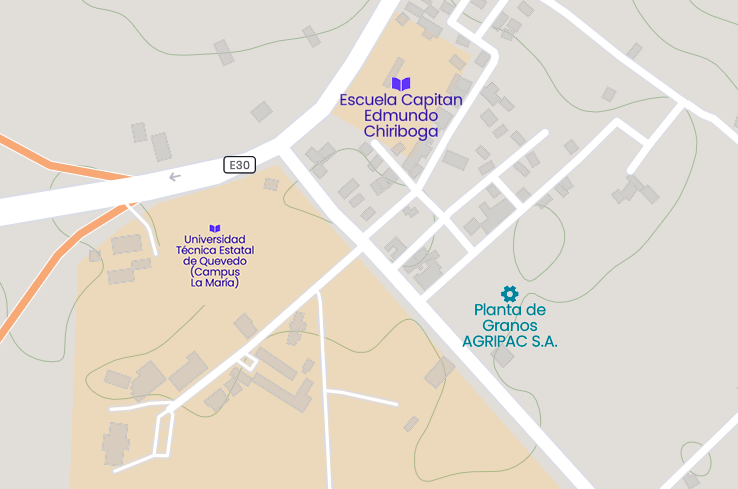
\includegraphics[width=12cm]{img/campuslamaria.png}
	\caption{Localización de la UTEQ campus "La María".}
	\label{fig:lamaria}
\end{figure}.

\section{Tipo de investigación}

La ejecución de este proyecto implico realizar una investigación de tipo exploratoria. Existen trabajos similares al presentado, pero no cumplen con conceptos semejantes a los que se ha planteado en este trabajo. Se utilizaron artículos científicos de revistas científicas indexadas y conferencias internacionales.

\section{Método de investigación}

\subsection{Método analítico}

\subsection{Método inductivo}

\section{Fuentes de recopilación de información}

\section{Diseño de la investigación}

Para el desarrollo del presente proyecto se tomarán en cuenta la ejecución de varias etapas, aplicando el Modelo de Prototipado para desarrollar un prototipo de la aplicación web que utilice el producto final de esta investigación. A continuación, se describe el enfoque metodológico correspondiente a cada una de las fases. 

\subsection{Búsqueda de aplicativos relacionados}

En esta fase se analizaron varias aplicaciones web que cuentan con la funcionalidad de generar diagramas de clases mediante la escritura de texto. Entre las aplicaciones analizadas se encuentran:

\begin{itemize}
	\item \textbf{yuml: }Es una aplicacion web que permite crear diagramas UML mediante la escritura por comandos en texto plano. Se puede destacar que esta herramienta no permite decidir la ubicación o lugar de un elemento grafico ya que busca la mejor distribución según el diagrama generado (https://yuml.me/)
	
	\item \textbf{mermaid: }Es una herramienta de gráficos y diagramas basada en JavaScript que utiliza definiciones de texto inspiradas en Markdown y un renderizador para crear y modificar diagramas complejos. El propósito principal de Mermaid es ayudar a que la documentación se ponga al día con el desarrollo. También se destaca que la aplicación no permite modificar en tiempo real los diagramas generados (https://mermaid.live/).
	
	\item \textbf{ditaa: }Es una pequeña utilidad de línea de comandos escrita en Java, que puede convertir diagramas dibujados con arte ascii ('dibujos' que contienen caracteres que se asemejan a líneas como | / - ), en gráficos de mapa de bits adecuados. También se destaca que la aplicación no permite modificar en tiempo real los diagramas generados (http://ditaa.sourceforge.net/). 
\end{itemize}

\subsection{Modelamiento}

En esta etapa se pretende modelar la funcionalidad que tendrán todos los métodos y funciones necesarias para identificar cada símbolo y poder interpretar todo el texto para generar la estructura del diagrama de clases.
Todo el archivo JavaScript estará conformado por estructuras de datos apuntando a la programación orientada a objetos.

\subsection{Desarrollo del código}

La tercera etapa se dedicará al desarrollo de la librería utilizando el lenguaje de programación JavaScript. Todo el código será escrito en un solo archivo con extensión de tipo .js teniendo como ventaja poder ser vinculado dentro de cualquier archivo HTML que dese utilizar los métodos necesarios para obtener la estructura de todo el diagrama de clases en formato JSON.

La estructura podrá ser utilizada por cualquier herramienta de dibujo externa que permita visualizar el diagrama de clases de la forma tradicional con todos sus componentes. A continuación, se enlista los componentes que podrán ser generados por la librería:

\begin{itemize}
	\item Entidades
	\item Interfaces
	\item Enumeradores
	\item Atributos
	\item Métodos
	\item Constructores de clases
	\item Relaciones
\end{itemize}

\subsection{Pruebas unitarias}
En esta fase se pretende realizar todas las pruebas posibles a las funciones que se realizaron en la fase anterior, ingresando algunos textos utilizando los símbolos esperando los valores que devuelva la librería. Algunos de los textos que serán ingresados son los siguientes:

\begin{itemize}
	\item \begin{verbatim}
		Create an user *(user %.username=String, .password=String,
		.status=Status, .user type=UserType, .person=Tutor%) object
	\end{verbatim}
	
	\item \begin{verbatim}
		*(TutorDAO &id=Int [/Save/=Tutor{.tutor=Tutor}])s the tutor 
		data in the database. *¡(TutorDAO)<<*(tutor)¡
	\end{verbatim}
	
	\item \begin{verbatim}
		*(UserDAO &-id=Int [/Save/=User{.user=User}])s the user data 
		in the database. *¡(UserDAO)<<*(User)¡
	\end{verbatim}
	
	\item \begin{verbatim}
		This use case ends when the system displays the *(@Login) 
		login Interface. *¡(Login)<<*(UserDAO)¡
	\end{verbatim}
	
\end{itemize}

\subsection{Evaluación con sistemas de información reales}

Se utilizaran estudios de caso con sistemas de información reales para crear las descripciones de los casos de uso extendidos de forma natural. Luego se implementaron los símbolos como se crea conveniente, dependiendo de los requisitos ingresados en el texto. Finalmente se utilizara la librería para observar como devuelve el texto nuevamente en forma natural adicional la estructura del diagrama de clases.

\subsection{Modelo de prototipado}
El Modelo de Prototipado se aplica cuando la información detallada relacionada a requerimientos de entrada y salida del sistema no está disponible. En este modelo se asume que tal vez no todos los requerimientos son conocidos en el inicio del desarrollo del sistema. Se usa generalmente cuando un sistema no existe, o en caso de un largo y complejo sistema, cuando no hay procesos manuales para determinar los requerimientos. Los pasos que se ejecutan en el modelo de prototipado son: 

\begin{enumerate}
	\item \textbf{Obtención y análisis de requisitos:} es el punto de partida del modelo. El usuario es entrevistado para conocer los requisitos del sistema.
	
	\item \textbf{Diseño rápido}: teniendo claro todos los requisitos, se procede a crear un diseño rápido y preliminar incluyendo solo los aspectos más importantes 
	
	\item\textbf{ Construir el prototipo:} se trabaja con la información tomada por el diseño rápido y crear el prototipo de la aplicación.
	
	\item \textbf{Evaluación de usuarios}: el sistema es presentado a varios usuarios para evaluar y verificar sus puntos fuertes y débiles Se reciben comentarios y sugerencias que serán analizadas por los desarrolladores.
	
	\item \textbf{Reajuste del prototipo:} el prototipo actual debe reajustarse según los nuevos requerimientos, es decir que, se debe crear un nuevo prototipo con la información adicional proporcionada por los usuarios evaluados. Este nuevo prototipo será reevaluado justo como el anterior. Este proceso se repite hasta que se cumplan todos los requerimientos especificados por el usuario. Cuando el usuario esté satisfecho con el resultado, se desarrollará un sistema final basado en el prototipo final. 
	
	\item \textbf{Implementación y mantenimiento:} Una vez que se tenga listo el sistema, ya estará listo para ser desplegado a producción. El sistema se somete a un mantenimiento de rutina para minimizar el tiempo de inactividad y evitar fallas a gran escala.
	
\end{enumerate}
	\setcounter{chapter}{4}
\setcounter{section}{0}
\part{RESULTADOS Y DISCUSIÓN} 

\section{Resultados de la metodología}

Los resultados que se obtuvieron al aplicar la metodología basada en el manifiesto del desarrollo de software ágil se redactan a continuación:

\subsection{Análisis de requisitos y obtención de pruebas}

Para llevar a cabo el análisis de los requisitos sobre la librería JavaScript que se desarrolló se tomaron en cuenta varios favores observando las carencias que existen al momento de realizar el modelamiento de cualquier software. Mediante el docente encargado de impartir las clases sobre cómo utilizar los lenguajes de modelado como lo es UML se dio cuenta que podría existir una forma en generar uno de los diagramas más importantes que es el diagrama de clases, pero a partir de las descripciones que se generan en los casos de uso del sistema.

Existe una herramienta denominada TDDT4IoTS que permite realizar el modelamiento de varios tipos de software. La herramienta cuenta con un lenguaje de símbolos que permiten escribir dentro de las descripciones de casos de uso datos técnicos sobre los objetos que intervendrán en el sistema informático que llevara a cabo la ejecución de todos los escenarios que se están describiendo. A petición del cliente recomendó que visitemos el sitio web de aplicaciones.uteq.edu.ec/tddt4iots para visualizar  los símbolos que usa la herramienta (ver figura \ref{fig:simbolostdd}).

\begin{figure}[H]
	\caption{Símbolos que utiliza la herramienta TDDT4IoTS}
	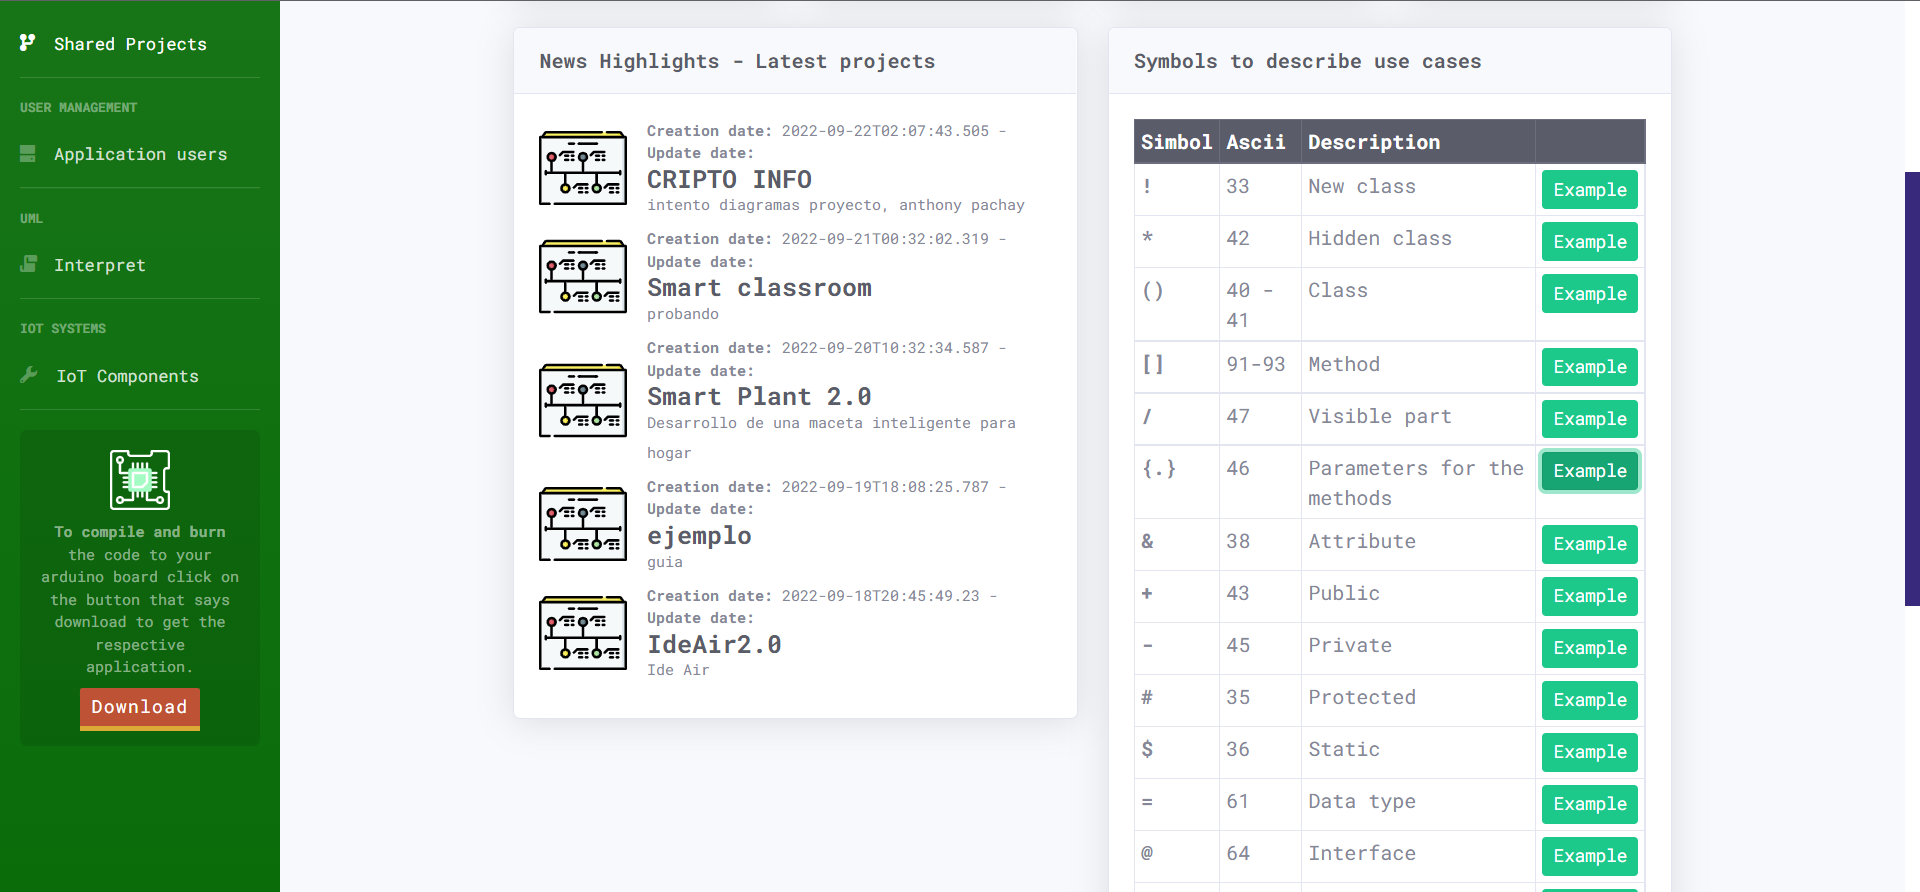
\includegraphics[width=14cm]{img/res_001.png}
	\label{fig:simbolostdd}
	\textbf{\\ FUENTE: PROPIA \\ ELABORADO: DÚVAL CARVAJAL SUÁREZ}
\end{figure}

En la lista de símbolos que se visualizar en la figura anterior se encuentra un botón que dice \textit{"Example"}. Si presionamos en ese botón se pudo observar un ejemplo detallado sobre cómo se deben utilizar los símbolos para tratar de especificar algún objeto del diagrama de clases que se generar mediante la descripción del caso de uso pertinente (ver figuras \ref{fig:ejemploclase}, \ref{fig:ejemploparametro}).

\begin{figure}[H]
	\caption{Ejemplo de cómo se debe utilizar el símbolo respectivo para crear una clase.}
	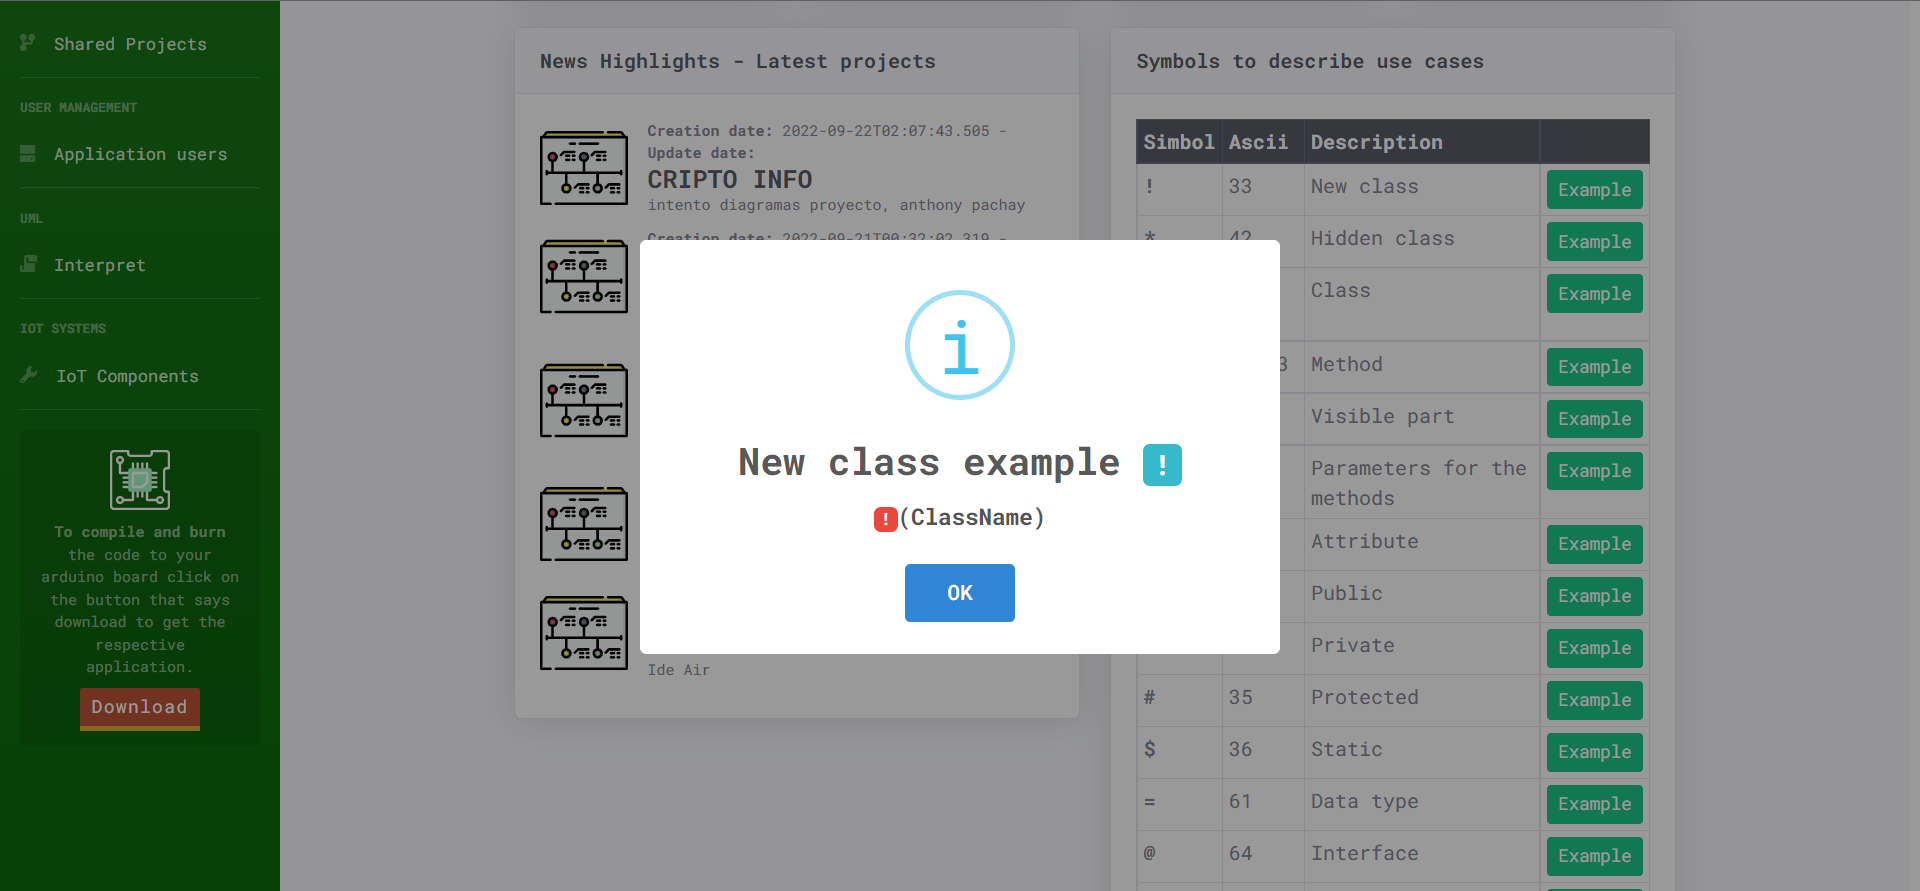
\includegraphics[width=14cm]{img/res_002.png}
	\label{fig:ejemploclase}
	\textbf{\\ FUENTE: PROPIA \\ ELABORADO: DÚVAL CARVAJAL SUÁREZ}
\end{figure}

\begin{figure}[H]
	\caption{Ejemplo de cómo se debe utilizar el símbolo respectivo generar los parámetros de un método declarado con el lenguaje de símbolos.}
	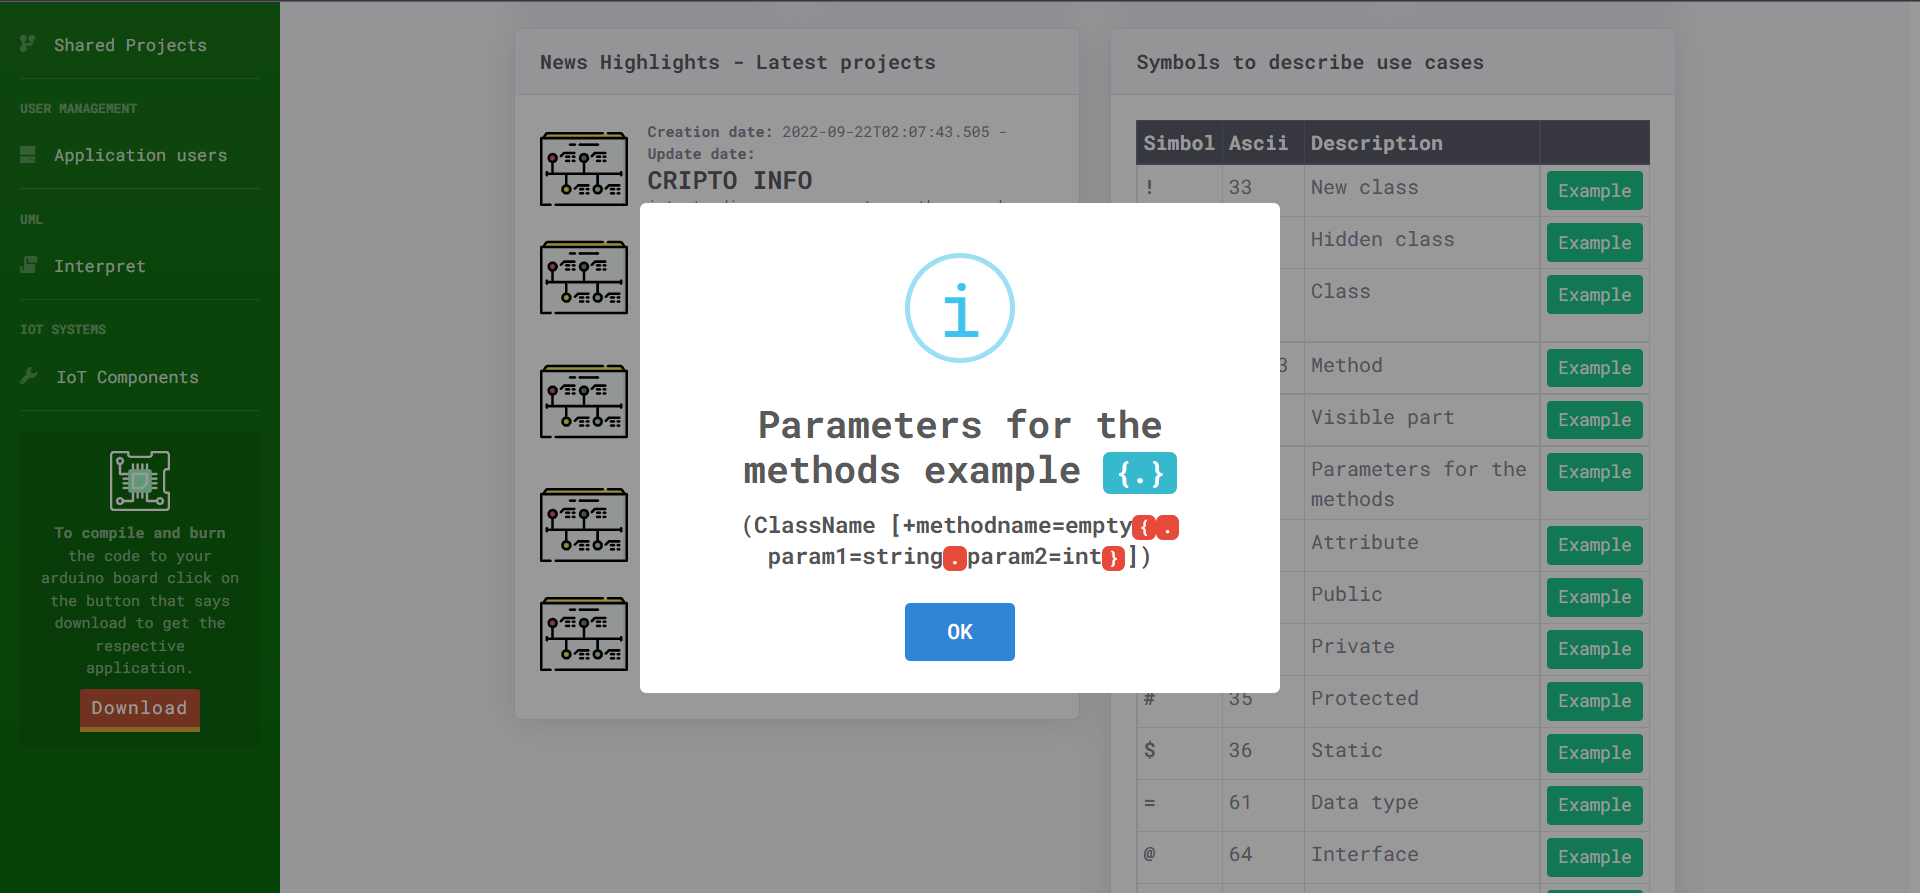
\includegraphics[width=14cm]{img/res_003.png}
	\label{fig:ejemploparametro}
	\textbf{\\ FUENTE: PROPIA \\ ELABORADO: DÚVAL CARVAJAL SUÁREZ}
\end{figure}

Luego de tener una idea general sobre los símbolos que utiliza la herramienta se especificaron detalladamente los significados de cada símbolo y como puede ser utilizado en las descripciones de los casos de uso.  

\begin{itemize}
	\item \textbf{Asterisco *}: Este símbolo sirve para ocultar cualquier carácter que se encuentre redactado después el. Esto permitirá al momento de interpretar la descripción del caso de uso ingresada eliminar los caracteres mezclados con los símbolos y solo dejar visibles los caracteres normales formando un texto natural que pueda ser entendido por cualquier persona regular. \textbf{Ejemplo:}
	
	\begin{verbatim}
		* texto de prueba
	\end{verbatim}
	
	\item \textbf{Paréntesis de apertura y cierre ()}: Este símbolo sirve para especificar uno de los componentes más importantes del diagrama de clases, dentro de los paréntesis de apertura y cierra se deberá especificar el nombre de la clase u objeto que se pretende generar de forma automática. Cabe mencionar que, si se escribe el nombre de clase separada por espacios, la librería deberá omitir estos espacios y auto completarlos con la segunda letra después del espacio con mayúscula. \textbf{Ejemplo:}  
	
	\begin{verbatim}
		(Nombre de la clase)
	\end{verbatim}
	
	\item \textbf{Corchete de apertura y cierre []:} Este símbolo podrá ser utilizado dentro de los símbolos para crear las clases, permitirá definir Los métodos o funciones que pertenecerá a la clase respectiva. \textbf{Ejemplo:} 
	
	\begin{verbatim}
		(Nombre de la clase [+nombre del método=empty])
	\end{verbatim} 
	
	\item \textbf{Slash /:} Este símbolo es bastante interesante, con él se deben visualizar  caracteres que se encuentre encerrado de un slash de apertura y otro slash de cierre. Este símbolo se lo deberá usar cuando todos los caracteres se encuentren después del símbolo del asterisco, la idea es permitir que se visualicen caracteres específicos dentro de los datos técnicos para generar el diagrama de clases, sin afectar el uso de los demás símbolos. \textbf{Ejemplo:}
	
	\begin{verbatim}
		(Nombre de la clase &+/nombre/=string)
	\end{verbatim} 
	
	\item \textbf{Llaves de apertura y llaves de cierre con punto \{.\}:} Con el símbolo de las llaves se podrá definir los parámetros de entrada para los métodos o funciones de las clases. Cada parámetro estará separado por un punto, además se deberá utilizar el símbolo del igual (=) para especificar su tipo de dato. Cada recalcar que todos los atributos también deberán estar especificados dentro de las llaves de apertura y cierre. \textbf{Ejemplo:}
	
	\begin{verbatim}
		(Nombre de la clase [+nombre del método=empty
		{.param1=string.param2=strgin}])
	\end{verbatim}
	
	\item \textbf{Ampersand \&: } Este símbolo debe permitir declarar los atributos de la clase que fue creada con el símbolo anterior. Existen otros símbolos que interviene en la creación de otros componentes del diagrama de clases, más adelante se detallaran para que sirven. \textbf{Ejemplo:}
	
	\begin{verbatim}
		(Nombre de la clase &+atributo uno=string &+atributo 
		dos=string)
	\end{verbatim}
	
	\item \textbf{Visibilidad +: } El símbolo de suma permite especificar que la visibilidad del atributo, método o función será de manera pública. \textbf{Ejemplo:}
	
	En este ejemplo se visualiza la forma en cómo utilizar el símbolo de suma en atributos de clase.
	
	\begin{verbatim}
		(Nombre de la clase &+atributo uno=string &+atributo 
		dos=string)
	\end{verbatim}
	
	En este ejemplo se visualiza la forma en cómo utilizar el símbolo de suma en métodos o funciones de clase.
	
	\begin{verbatim}
		(Nombre de la clase [+nombre del método=empty
		{.param1=string.param2=strgin}])
	\end{verbatim}
	
	\item \textbf{Visibilidad -: } El símbolo de resta permite especificar que la visibilidad del atributo, método o función será de manera privada. \textbf{Ejemplo:}
	
	En este ejemplo se visualiza la forma en cómo utilizar el símbolo de suma en atributos de clase.
	
	\begin{verbatim}
		(Nombre de la clase &-atributo uno=string &-atributo 
		dos=string)
	\end{verbatim}
	
	En este ejemplo se visualiza la forma en cómo utilizar el símbolo de suma en métodos o funciones de clase.
	
	\begin{verbatim}
		(Nombre de la clase [-nombre del método=empty
		{.param1=string.param2=strgin}])
	\end{verbatim}
	
	\item \textbf{Visibilidad \#: } El símbolo de almohadilla permite especificar que la visibilidad del atributo, método o función será de manera protegida. \textbf{Ejemplo:}
	
	En este ejemplo se visualiza la forma en cómo utilizar el símbolo de suma en atributos de clase.
	
	\begin{verbatim}
		(Nombre de la clase &#atributo uno=string &#atributo 
		dos=string)
	\end{verbatim}
	
	En este ejemplo se visualiza la forma en cómo utilizar el símbolo de suma en métodos o funciones de clase.
	
	\begin{verbatim}
		(Nombre de la clase [#nombre del método=empty
		{.param1=string.param2=strgin}])
	\end{verbatim}
	
	\item \textbf{Visibilidad \$: } El símbolo de dólar permite especificar que la visibilidad del atributo, método o función será de manera estática. \textbf{Ejemplo:}
	
	En este ejemplo se visualiza la forma en cómo utilizar el símbolo de suma en atributos de clase.
	
	\begin{verbatim}
		(Nombre de la clase &$atributo uno=string &$atributo 
		dos=string)
	\end{verbatim}
	
	En este ejemplo se visualiza la forma en cómo utilizar el símbolo de suma en métodos o funciones de clase.
	
	\begin{verbatim}
		(Nombre de la clase [$nombre del metodo=empty
		{.param1=string.param2=strgin}])
	\end{verbatim}
	
	\item \textbf{Igual =:} El símbolo de igual debe permitir asignar el tipo de dato a los atributos, métodos o funciones declaradas dentro de la clase. En el caso de los métodos de tipo \textbf{void}  se deberá utilizar la palabra \textit{empty} indiciando que es un método que retornara ningún valor. \textbf{Ejemplo:}
	
	\begin{verbatim}
		{.param1=string.param2=strging}
	\end{verbatim}
	
	\item \textbf{Arroba @:} El símbolo de arroba se lo utiliza dentro de los paréntesis que permiten generar una clase del diagrama. Pero se recuerda que en el diagrama de clases también se pueden crear interfaces. El objetivo de este símbolo es utilizarlo dentro de los paréntesis, pero el interprete identificara que sera una interfaz la que se deberá crear. \textbf{Ejemplo:}
	  
	\begin{verbatim}
		(@nombre interfaz)
	\end{verbatim}

	\item  \textbf{Signo de interrogación apertura y cierre ¿?:} El símbolo de interrogación se lo utiliza para generar otro tipo de objeto principal del diagrama de clases. El objetivo principal de este símbolo es generar los enum. \textbf{Ejemplo:}
	
	\begin{verbatim}
		¿enumTest?
	\end{verbatim}

	\item \textbf{Cierra comillas bajas »:} El simbolo de cierre comillas bajas se lo utiliza para agregar atributos a un objeto principal del diagrama de clases. El objetivo principal de este símbolo es atributos dentro de los objetos enum. \textbf{Ejemplo:}
	
	\begin{verbatim}
		¿enumTest »atributoUno »atributoDos?
	\end{verbatim}

	\item \textbf{Porcentaje \%:} El símbolo de porcentaje sirve para agregar nuevos constructores a las clases que ya fueron definidas, además para especificar sus parámetros se utiliza los mismos símbolos para agregar atributos a la clase, con la diferencia que los parámetros van separados por la coma. \textbf{Ejemplo:}
	
	\begin{verbatim}
		*(class %.class=Class, .param=string%)
	\end{verbatim}
	  
\end{itemize}

Dentro del diagrama de clases existen diferentes tipos de relaciones con las que se pueden relacionar las clases que se encuentran definidas. Para implementar las relaciones también se utilizan una combinación de símbolos que permitan detectarlas y la librería se encarga de generarlas. A continuación, se especificarán los símbolos que se utilizan para los tipos de relaciones en el diagrama de clases:

\begin{itemize}
	\item \textbf{Símbolo de admiración de apertura ¡!:} Para indicar que se va realizar una relación entre 2 objetos del diagrama de clases, el texto debe estar entre este símbolo tanto en su apertura y cierre.
	
	\item \textbf{Corchete de apertura y cierre []:} Dentro del símbolo de admiración se podrá indicar un texto como leyenda sobre la línea de la relación, esto indicara alguna palabra clave sobre la relación entre los objetos.
	
	\item \textbf{Cardinalidad 1 o n:} Sobre la línea de la relación se puede indicar una cardinalidad de uno a muchos. El numero \textit{\underline{1}} indicará que la cardinalidad es de 1 y si usa la letra \textit{\underline{n}} indicará que la cardinalidad des de muchos. Se los debe utilizar en la parte exterior de los corchetes.
	
	\item \textbf{Agregación > >:} Para indicar que el tipo de relación entre dos objetos del diagrama de clases se utiliza los símbolos de \textit{> >}. Se deben colocar en la parte exterior donde se el texto de cardinalidad. \textbf{Ejemplo:}
	
	
	\begin{verbatim}
		*¡claseUno 1>[texto de cardinalidad]>n claseDos!
	\end{verbatim}

	\item \textbf{Dependencia < <:} Para indicar que el tipo de relación entre dos objetos del diagrama de clases se utiliza los símbolos de \textit{< <}. Se deben colocar en la parte exterior donde se el texto de cardinalidad. \textbf{Ejemplo:}
	
	\begin{verbatim}
		*¡claseUno 1<[texto de cardinalidad]<n claseDos!
	\end{verbatim}

	\item \textbf{Generalización < >:} Para indicar que el tipo de relación entre dos objetos del diagrama de clases se utiliza los símbolos de \textit{<>}. Se deben colocar en la parte exterior donde se el texto de cardinalidad. \textbf{Ejemplo:}
	
	\begin{verbatim}
		*¡claseUno 1<[texto de cardinalidad]>n claseDos!
	\end{verbatim}

	\item \textbf{Asociación > <:} Para indicar que el tipo de relación entre dos objetos del diagrama de clases se utiliza los símbolos de \textit{> <}. Se deben colocar en la parte exterior donde se el texto de cardinalidad. \textbf{Ejemplo:}
	
	\begin{verbatim}
		*¡claseUno 1>[texto de cardinalidad]<n claseDos!
	\end{verbatim}
	
\end{itemize}

En la tabla se describe el código ASCII para escribir los símbolos mediante el teclado de una computadora. Se pretendió que cada símbolo tenga una combinación ASCII para que el analista pueda escribir cada símbolo con el teclado y no obtenerlo de alguna forma que sea complicada.

\begin{table}[h!]
	\caption{Código ASCII para cada símbolo del lenguaje.}
	\begin{tabular}{p{2cm}p{4cm}p{5cm}}
		\toprule
		\textbf{Símbolo} & \textbf{ASCII} & \textbf{Descripción} \\
		\midrule
		* & 33 & Ocultar texto \\
		\addlinespace
		( ) & 40 - 41 & Crear clase \\
		\addlinespace
		\textbf{[ ]} & 91 - 93 & Crear método \\
		\addlinespace
		/ & 47 & Parte visible \\
		\addlinespace
		\{.\} & 123 - 125	 & Parámetro de los métodos \\
		\addlinespace 	
		\& & 38 & Atributo de clase \\
		\addlinespace
		+ & 43 & Publico \\
		\addlinespace
		- & 45 & Privado \\
		\addlinespace
		\# & 35 & Protegido \\
		\addlinespace
		\$ & 36 & Estático \\
		\addlinespace
		= & 61 & Tipo de dato \\
		\addlinespace
		@ & 64 & Interfaz \\
		\addlinespace
		¿? & 168 - 63 & Enum \\
		\addlinespace
		\% & 37 & Constructores \\
		\addlinespace
		\bottomrule
	\end{tabular}
	\textbf{ \\ ELABORADO: DÚVAL CARVAJAL SUÁREZ}
\end{table}

Para definir los diferentes tipos de relaciones que se usaran en el diagrama de clases. En la tabla se visualiza un grupo de símbolos que servirán para crear las relaciones de tipo: agregación, dependencia, herencia o generalización y asociación. 

\begin{table}[h!]
	\caption{Código ASCII para cada símbolo del lenguaje que especifican las relaciones.}
	\begin{tabular}{p{2cm}p{4cm}p{6cm}}
		\toprule
		\textbf{Símbolo} & \textbf{ASCII} & \textbf{Descripción} \\
		\midrule
		¡! & 33 - 173 & Crear relación \\
		\addlinespace
		\textbf{[ ]} & 91 - 93 & Especificar leyenda en la relación \\
		\addlinespace
		1[ ]1 & -- & Cardinalidad de uno a uno \\
		\addlinespace
		1[ ]n & -- & Cardinalidad de uno a muchos \\
		\addlinespace
		n[ ]1 & -- & Cardinalidad de muchos a uno \\
		\addlinespace
		> > & 62 - 62 & Agregación \\
		\addlinespace
		< < & 60 - 60 & Dependencia \\
		\addlinespace
		< > & 60 - 62 & Generalización \\
		\addlinespace
		> < & 62 - 60 & Asociación \\
		\addlinespace
		\bottomrule
	\end{tabular}
	\textbf{ \\ ELABORADO: DÚVAL CARVAJAL SUÁREZ}
\end{table}

Luego de a ver recopilado todos los símbolos que la librería va a interpretar, el docente proporciono 1 caso de uso. Además, proporciono el gráfico del diagrama de clases que se escribió en los casos de uso. En la figura \ref{fig:usecasetest} se observa el caso de uso de prueba para saber que objetos debe generar la librería. 

\begin{figure}[h!]
	\caption{Diagrama de casos de uso para las pruebas.}
	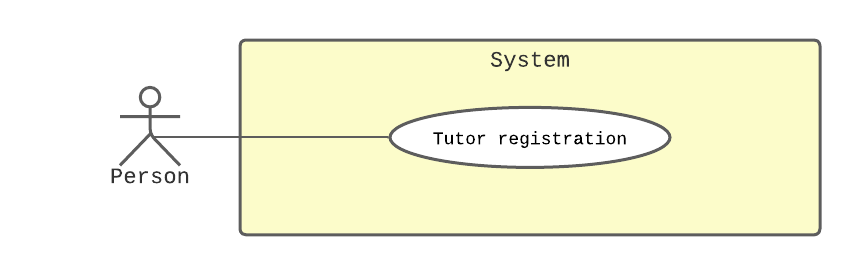
\includegraphics[width=15cm]{img/usecaseTest.png}
	\label{fig:usecasetest}
	\textbf{\\ ELABORADO: DÚVAL CARVAJAL SUÁREZ}
\end{figure}

Para comprender totalmente las acciones que se deben ejecutar en el caso de uso que se usara como prueba, está escrito en 2 distintas formas. En la tabla \ref{tab:usecasetutorregistration} se observa la descripción del caso de uso en lenguaje natural especificando todas las acciones con el objetivo que cualquier persona regular logre entender. En la tabla \ref{tab:usecasetutorregistration_symbol} se observa la misma descripción del caso de uso pero utilizando los símbolos. 

\newpage  

\begin{table}[h!]
	\caption{Descripción del caso de uso para Tutor registration.}
	\label{tab:usecasetutorregistration}
	\begin{tabular}{| p{3cm} | p{11cm} |}
		\hline
		\textbf{Use case:} & Tutor registration \\ \hline
		\textbf{Actors:} & Person \\ \hline
		\textbf{Postcondition:} & User registered in the database. \\ \hline
		\textbf{Precondition:} & The user exists in the database. \\ \hline
		\textbf{Purpose:} & Ingresar a la interfaz principal de la aplicación \\ \hline
		\textbf{Abstract:} & 
		Permite identificar las credenciales del usuario que intenta ingresar al sistema, de esa forma verificar el tipo de usuario que ingresa. \\ \hline
		\textbf{Type:} & Primary \\ \hline
		\multicolumn{2}{ |c| }{\textbf{Normal flow}} \\ \hline
	\end{tabular}
	\begin{tabular}{| p{7cm} | p{7cm} |}
		1. This use case starts when a person wants to register as a tutor user in the system.  & \\ \hline
		2. The person accesses then User Registration interface. & \\ \hline
		& 3. Shows you the fields to fill in the interface user registration: first name last name date of birth gender phone number email username password. It should be taken into account that the registration of a Person has a User. There are states that can be Disabled o Enabled that each User will have a Status. There are also several types of users, which are Tutor or Patient or Admin and every User will have a UserType. In addition, the system assigns an id when storing it. \\ \hline
		4. The person enters all the data required by the view, and clicks submit. & \\ \hline
		& 5. Create a person object. \\ \hline
		& 6. Create a tutor object. \\ \hline
		& 7. Create an user object. \\ \hline
		& 8. Saves the tutor data in the database. \\ \hline
		& 9. Saves the user data in the database. \\ \hline
		& 10. This use case ends when the system displays the login Interface.  \\ \hline
	\end{tabular} \\
	\textbf{ \\ ELABORADO: DÚVAL CARVAJAL SUÁREZ}
\end{table}

Para la elaboración de la descripción del caso de uso con los símbolos proporcionaron información de un diagrama de clases que ya se encontraba realizado. El objetivo de este caso de uso era escribir todas las acciones con información técnica que permita crear el diagrama de clases lo más parecido posible al original. En la figura \ref{fig:cdtest} se observa el diagrama de clases creado de forma manual.

\begin{figure}[h!]
	\caption{Diagrama de clases de prueba}
	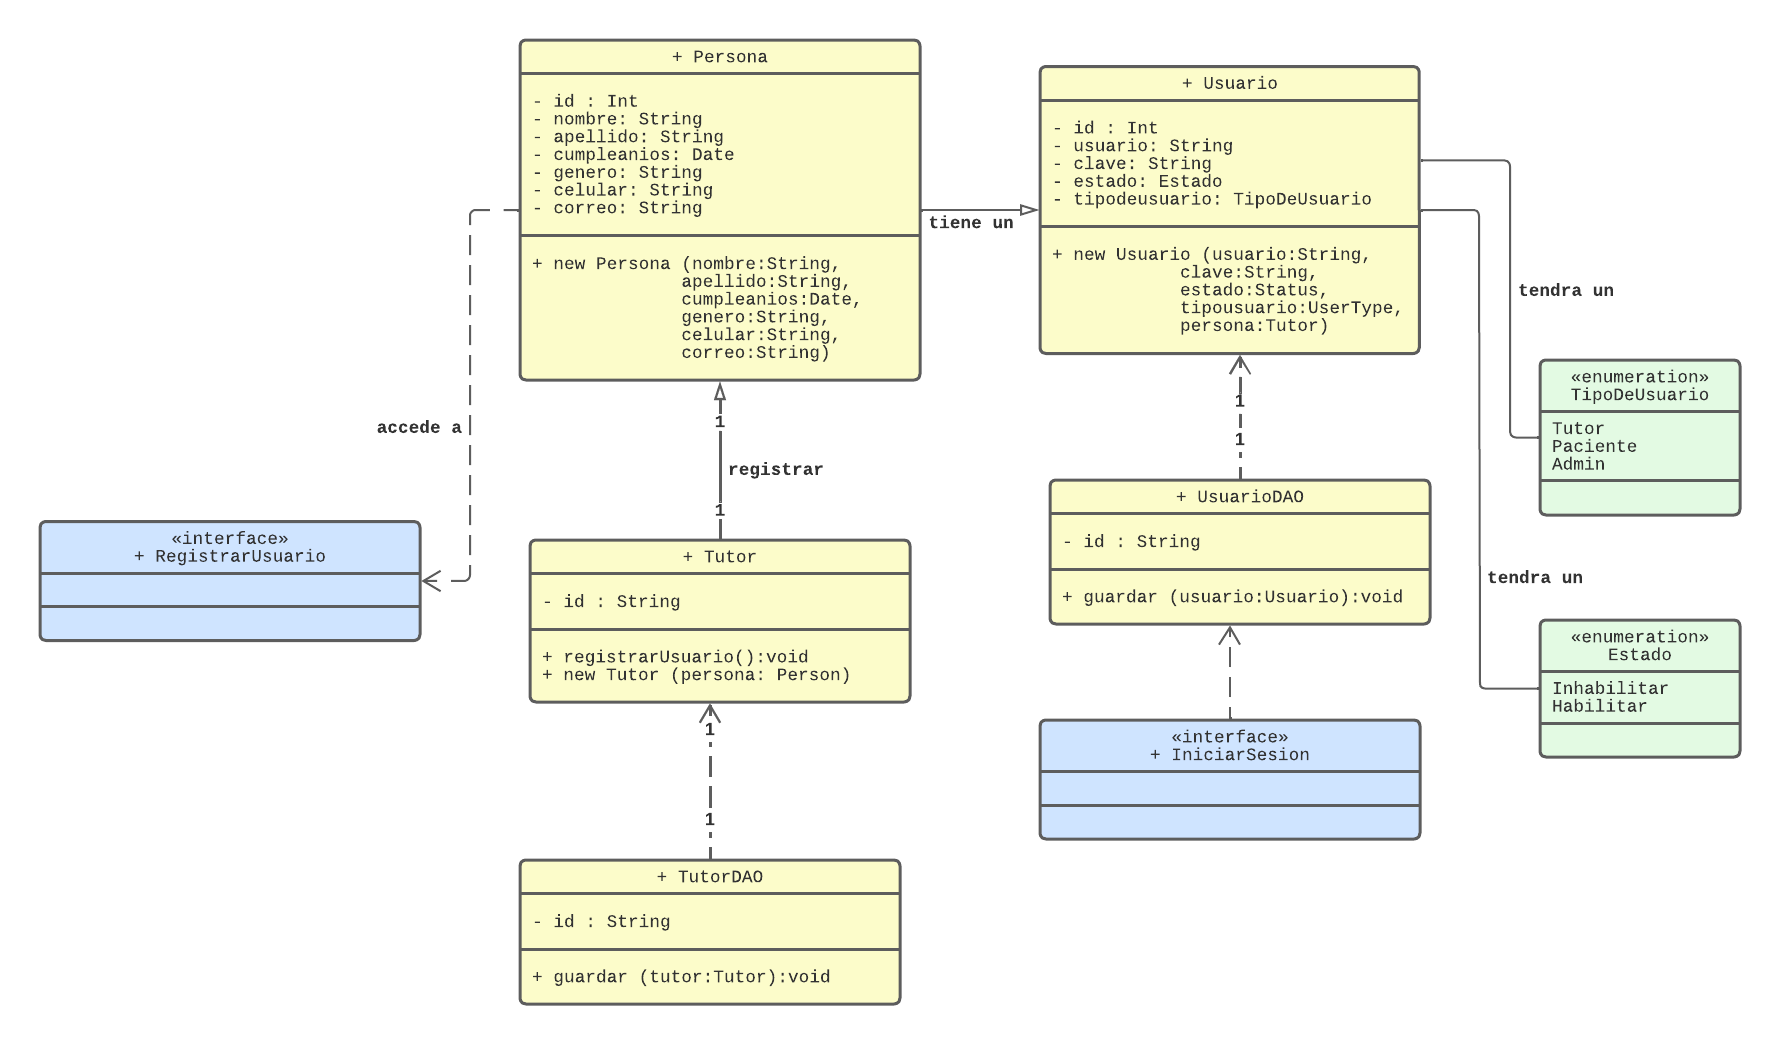
\includegraphics[width=15.5cm]{img/cdtest.png}
	\label{fig:cdtest}
	\textbf{\\ ELABORADO: DÚVAL CARVAJAL SUÁREZ}
\end{figure}

\begin{table}[h!]
	\caption{Descripción del caso de uso para Tutor registration.}
	\label{tab:usecasetutorregistration_symbol}
	\begin{tabular}{| p{3cm} | p{11cm} |}
		\hline
		\textbf{Use case:} & Tutor registration \\ \hline
		\textbf{Actors:} & Person \\ \hline
		\textbf{Postcondition:} & User registered in the database. \\ \hline
		\textbf{Precondition:} & The user exists in the database. \\ \hline
		\textbf{Purpose:} & Ingresar a la interfaz principal de la aplicación \\ \hline
		\textbf{Abstract:} & 
		Permite identificar las credenciales del usuario que intenta ingresar al sistema, de esa forma verificar el tipo de usuario que ingresa. \\ \hline
		\textbf{Type:} & Primary \\ \hline
		\multicolumn{2}{ |c| }{\textbf{Normal flow}} \\ \hline
	\end{tabular}
	\begin{tabular}{| p{7cm} | p{7cm} |}
		1. This use case starts when a person *(person \&-id=int) wants to register as a tutor *(tutor \&-id=int [+userRegistration=Tutor]) user in the system. *¡tutor 1<[register]>n Person! & \\ \hline
		2. The person accesses then User Registration *(@User Registration) interface. *¡person1<[accesses]<1 User Registration! & \\ \hline

	\end{tabular}
\end{table}

\begin{table}[]
	\begin{tabular}{| p{7cm} | p{7cm} |}
		\hline
		& 3. Shows you the fields to fill in the interface user registration *(@User registration): *(Person \&-/first name/=String, \&-/last name/=String, \&-/date of birth/=Date, \&-/gender/=String, \&-/phone number/=String, \&-/email/=String) *(User \&-id=Int, \&-/username/=String, \&-/password/=String \&-status=Status \&-user type=UserType). It should be taken into account that the registration of a *!/Person/ u<[/has a/]>u /User/¡. There are states that can be *¿Status »/Disabled/ /o/ »/Enabled/? that each *¡/User/ u>[/will have a/]<u /Status/! . There are also several types of users, which are *¿UserType »/Tutor/ /or/ »/Patient/ /or/ »/Admin/? and every *¡/User/ u>[/will have a/]<u /UserType/!. In addition, the system assigns an id when storing it. \\ \hline
		4. The person enters all the data required by the view, and clicks submit. & \\ \hline
		& 5. Create a *(/person/ \%.first name=String, .last name=String, .date of birth=Date, .gender=String, .phone number=String, .email=String\%) object. \\ \hline
		& 6. Create a *(/tuto/r \%.person=Person\%) object \\ \hline
		& 7. Create an *(/user/ \%.username=String, .password=String, .status=Status, .user type=UserType, .person=Tutor\%) object \\ \hline
		& 8. *(TutorDAO \&id=Int [/Save/=Tutor{.tutor=Tutor}])s the tutor data in the database. *¡TutorDAO<[]< tutor!. \\ \hline
		& 9. *(UserDAO \&-id=Int [/Save/=User{.user=User}])s the user data in the database. *¡UserDAO <[]< User!. \\ \hline
		& 10. This use case ends when the system displays the *(@Login) login Interface. *¡Login u<[]<u UserDAO! \\ \hline
	\end{tabular} \\
\textbf{\\ ELABORADO: DÚVAL CARVAJAL SUÁREZ}
\end{table}

\subsection{Modelamiento}

Se utilizo el lenguaje de programación JavaScript con la intención de generar un paquete totalmente exportable a otros proyectos que requieran utilizar la librería para generar sus propios diagramas con otras librerías de dibujo. Para empezar con el diseño o modelamiento de la librería se especificó el proceso normal que deberá seguir la al momento de recibir como datos de entrada las descripciones de los casos de uso. En la figura \ref{fig:armadillocasodeuso} se observa el proceso que se llevara a cabo de forma general la ejecución de la librería.

En la figura \ref{fig:armadillocasodeuso} se pude observar el diagrama de casos de uso que explica las acciones que el analista podrá realizar al momento de implementar la librería, o podrá utilizar la aplicación de demostración


\begin{figure}[h!]
	\caption{Diagrama de casos de uso armadillo.}
	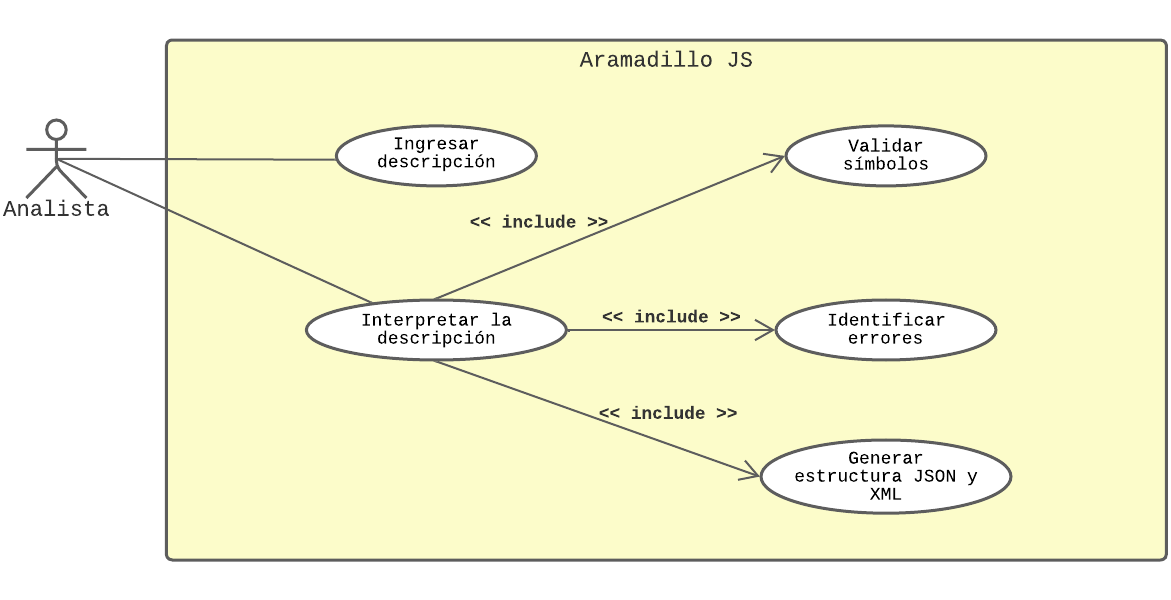
\includegraphics[width=15cm]{img/modelamientocasodeuso.png}
	\label{fig:armadillocasodeuso}
	\textbf{\\ \\ ELABORADO: DÚVAL CARVAJAL SUÁREZ}
\end{figure} 

A continuación, se detallarán las descripciones de los casos de uso que se observan en la imagen anterior. Se especificarán todos los pasos que la librería debe recibir para responder de forma correcta. Se recuerda que la librería no cuenta con acceso a datos o algún tipo de información en la nube.  

En la tabla \ref{tab:ucingresardescripcion} se detallan los pasos que se siguen al momento de ingresar las descripciones de los casos de uso que se pretenden interpretar.


\newpage

\begin{table}[H]
	\caption{Descripción del caso de uso para ingresar la descripción.}
	\label{tab:ucingresardescripcion}
	\begin{tabular}{| p{3cm} | p{11cm} |}
		\textbf{Acción del actor} & \textbf{Respuesta del sistema} \\ \hline	
		\textbf{Caso de uso:} & Ingresar descripción \\ \hline
		\textbf{Actores:} & Analista \\ \hline
		\textbf{Precondición:} & Tener instanciada la librería en su proyecto web, o debe utilizar la aplicación de demostración. \\ \hline
		\textbf{Postcondición:} & Descripción ingresada en la librería. \\ \hline
		\textbf{Propósito:} & Ingresar un párrafo de la descripción del caso de uso. \\ \hline
		\textbf{Resumen:} & Permite ingresar un párrafo de toda la descripción del caso de uso utilizando el lenguaje de símbolos. \\ \hline
		\textbf{Tipo:} & Primario \\ \hline
		\multicolumn{2}{ |c| }{\textbf{Flujo normal}} \\ \hline
	\end{tabular}
	\begin{tabular}{| p{7cm} | p{7cm} |}
		\textbf{Acción del actor} & \textbf{Respuesta del sistema} \\ \hline	
		1. Este caso de uso inicia el analista pretende ingresar la descripción del caso de uso. & \\ \hline
		2. Redacta la descripción del caso uso utilizando el lenguaje de símbolos.  & \\ \hline
		& 3. Muestra la caja de texto donde se debe colocar la descripción del caso de uso con el lenguaje de símbolos. \\ \hline
		4. Este caso de uso finaliza cuando el analista ingresa la descripción del caso de uso. & \\ \hline		
		\multicolumn{2}{ |c| }{\textbf{Flujos alternos}} \\ \hline
	\end{tabular}
	\begin{tabular}{| p{7cm} | p{7cm} |}
		
	\end{tabular} \\
	\textbf{ \\ ELABORADO: DÚVAL CARVAJAL SUÁREZ}
\end{table}

\newpage

\begin{table}[h!]
	\caption{Descripción del caso de uso para interpretar la descripción.}
	\label{tab:ucinterpretardescripcion}
	\begin{tabular}{| p{3cm} | p{11cm} |}
		\hline
		\textbf{Caso de uso:} & Interpretar descripción \\ \hline
		\textbf{Actores:} & Analista \\ \hline
		\textbf{Precondición:} & Tener ingresada la descripción a interpretar redactada con el lenguaje de símbolos. \\ \hline
		\textbf{Postcondición:} & Obtener la descripción redactada en lenguaje natural. \\ \hline
		\textbf{Propósito:} & Obtener la descripción del caso de uso e interpretar los símbolos del lenguaje. \\ \hline
		\textbf{Resumen:} & Permite identificar cada símbolo del lenguaje para identificar los objetos que se deben crear en el diagrama de clases. \\ \hline
		\textbf{Tipo:} & Primario \\ \hline
		\multicolumn{2}{ |c| }{\textbf{Flujo normal}} \\ \hline
	\end{tabular}
	\begin{tabular}{| p{7cm} | p{7cm} |}
		\textbf{Acción del actor} & \textbf{Respuesta del sistema} \\ \hline	
		1. Este caso de uso inicia cuando el analista pretende interpretar la descripción del caso de uso. & \\ \hline		
		2. El analista da la orden de interpretar la descripción con el lenguaje de símbolos. & \\ \hline
		& 3. Muestra dentro de un apartado denominado consola, todos los procesos que realizaron al momento de interpretar la descripción. Además de mostrar rápidamente el texto redactado en lenguaje normal. \\ \hline
		4. El analista se dirige a la pestaña de "Class diagram".  & \\ \hline
		& 5. Muestra el grafico del diagrama de clases generado por la librería. Se dibujan los objetos que pudieron ser identificados por los símbolos usados. \\ \hline
		6. El analista se dirige a la pestaña de "JSON". & \\ \hline
		& 7. Muestra la estructura JSON generada. \\ \hline
		8. El analista se dirige a la pestaña de "XML".  & \\ \hline
		& 9. Muestra la estructura XML generada. \\ \hline
		10. Este caso de uso finaliza cuando el analista descarga las estructuras JSON o XML para posteriores proyectos. & \\ \hline			
		\multicolumn{2}{ |c| }{\textbf{Flujos alternos}} \\ \hline
	\end{tabular}
	\begin{tabular}{| p{7cm} | p{7cm} |}
		
	\end{tabular} \\
	\textbf{ \\ ELABORADO: DÚVAL CARVAJAL SUÁREZ}
\end{table}

\begin{table}[H]
	\caption{Descripción del caso de uso para validar símbolos.}
	\label{tab:ucvalidarsimbolos}
	\begin{tabular}{| p{3cm} | p{11cm} |}
		\hline
		\textbf{Caso de uso:} & Validar símbolos \\ \hline
		\textbf{Actores:} & Analista \\ \hline
		\textbf{Precondición:} & La descripción del caso de uso debe contar con los símbolos del lenguaje. \\ \hline
		\textbf{Postcondición:} & Todos los símbolos serán omitidos en el texto que sea interpretado. \\ \hline
		\textbf{Propósito:} & Identificar los objetos para generar el diagrama de clases \\ \hline
		\textbf{Resumen:} & Permite identificar los símbolos que son usados para redactar los casos de uso. Además de verificar si se los esta usando de forma correcta. \\ \hline
		\textbf{Tipo:} & Secundario \\ \hline
		\multicolumn{2}{ |c| }{\textbf{Flujo normal}} \\ \hline
	\end{tabular}
	\begin{tabular}{| p{7cm} | p{7cm} |}
		\textbf{Acción del actor} & \textbf{Respuesta del sistema} \\ \hline	
		& 1. Este caso de uso inicia cuando la descripción del caso fue ingresada con los símbolos del lenguaje. \\ \hline
		& 2. Se identifican los tipos de símbolos que tiene el lenguaje, si son símbolos con apertura y cierre o son individuales. \\ \hline
		& 3. Se verifica que los símbolos están usándose de forma correcta sin combinarlos con otros símbolos desconocidos.  \\ \hline
		& 4. Este caso de uso finaliza cuando se identificaron todos los símbolos de la descripción y oculta los símbolos para obtener un texto natural.  \\ \hline		
		\multicolumn{2}{ |c| }{\textbf{Flujos alternos}} \\ \hline
	\end{tabular}
	\begin{tabular}{| p{7cm} | p{7cm} |}
		
	\end{tabular} \\
	\textbf{ \\ ELABORADO: DÚVAL CARVAJAL SUÁREZ}
\end{table}

\begin{table}[H]
	\caption{Descripción del caso de uso para identificar errores.}
	\label{tab:ucidentificarerror}
	\begin{tabular}{| p{3cm} | p{11cm} |}
		\hline
		\textbf{Caso de uso:} & Identificar errores \\ \hline
		\textbf{Actores:} & Analista \\ \hline
		\textbf{Precondición:} & La descripción del caso de uso debe contar con los símbolos del lenguaje. \\ \hline
		\textbf{Postcondición:} & Todos los símbolos serán omitidos en el texto que sea interpretado. \\ \hline
		\textbf{Propósito:} & Permite identificar la mala escritura de las descripciones de los casos de uso. \\ \hline
		\textbf{Resumen:} & Identificar los posibles errores que se pueden cometer al momento de usar los símbolos en las descripciones de los casos de uso. \\ \hline
		\textbf{Tipo:} & Secundario \\ \hline
		\multicolumn{2}{ |c| }{\textbf{Flujo normal}} \\ \hline
	\end{tabular}
	\begin{tabular}{| p{7cm} | p{7cm} |}
		\textbf{Acción del actor} & \textbf{Respuesta del sistema} \\ \hline	
		& 1. Este caso de uso inicia cuando la descripción del caso fue ingresada con los símbolos del lenguaje. \\ \hline
		& 2. Se identifican los tipos de símbolos que tiene el lenguaje, si son símbolos con apertura y cierre o son individuales. \\ \hline
		& 3. Si existen inconsistencias en la redacción de la descripción del caso de uso, se empieza acumular mensajes de alerta.   \\ \hline
		& 4.  Este caso de uso finaliza mostrando los mensajes en un apartado y clasificando los mensajes acumulados mediante un color diferentes: Azul para información, amarillo para advertencia, verde para exitoso y rojo para notificar errores graves. \\ \hline		
		\multicolumn{2}{ |c| }{\textbf{Flujos alternos}} \\ \hline
	\end{tabular}
	\begin{tabular}{| p{7cm} | p{7cm} |}
		
	\end{tabular} \\
	\textbf{ \\ ELABORADO: DÚVAL CARVAJAL SUÁREZ}
\end{table}

\begin{table}[H]
	\caption{Descripción del caso de uso para generar estructura json y xml.}
	\label{tab:ucgenerarjsonxml}
	\begin{tabular}{| p{3cm} | p{11cm} |}
		\hline
		\textbf{Caso de uso:} & Generar estructura JSON y XML \\ \hline
		\textbf{Actores:} & Analista \\ \hline
		\textbf{Precondición:} & La descripción del caso de uso debe contar con los símbolos del lenguaje. \\ \hline
		\textbf{Postcondición:} & Todos los símbolos serán omitidos en el texto que sea interpretado. \\ \hline
		\textbf{Propósito:} & Generar 2 estructuras con la información necesaria del diagrama de clases. \\ \hline
		\textbf{Resumen:} & Permite obtener toda la estructura del diagrama de clases generado en formato JSON Y XML \\ \hline
		\textbf{Tipo:} & Secundario \\ \hline
		\multicolumn{2}{ |c| }{\textbf{Flujo normal}} \\ \hline
	\end{tabular}
	\begin{tabular}{| p{7cm} | p{7cm} |}
		\textbf{Acción del actor} & \textbf{Respuesta del sistema} \\ \hline	
		& 1. Este caso de uso inicia cuando la descripción del caso fue ingresada con los símbolos del lenguaje. \\ \hline
		& 2. Buscar los objetos que fueron identificados por los símbolos e ir armando el json y xml. \\ \hline
		& 3. Este caso de uso finaliza cuando se muestra por completo el json y xml uniendo todos los objetos del diagrama de clases  \\ \hline		
		\multicolumn{2}{ |c| }{\textbf{Flujos alternos}} \\ \hline
	\end{tabular}
	\begin{tabular}{| p{7cm} | p{7cm} |}
		
	\end{tabular} \\
	\textbf{ \\ ELABORADO: DÚVAL CARVAJAL SUÁREZ}
\end{table}

Para cumplir con los requisitos recopilados en la fase anterior se realizaron diagramas de flujo para realizar el análisis pertinente a lo que la librería debe cumplir. Esto permitirá identificar las posibles fallas que se mostrarían al momento de estar utilizando la librería. En la figura \ref{fig:algoritmoerror} se observa el algoritmo que permitió identificar los errores en la escritura de las descripciones de los casos de uso utilizando el lenguaje de símbolos.

\begin{figure}[h!]
	\caption{Diagrama de flujo para detectar errores en las descripciones de los casos de uso utilizando un el lenguaje de símbolos.}
	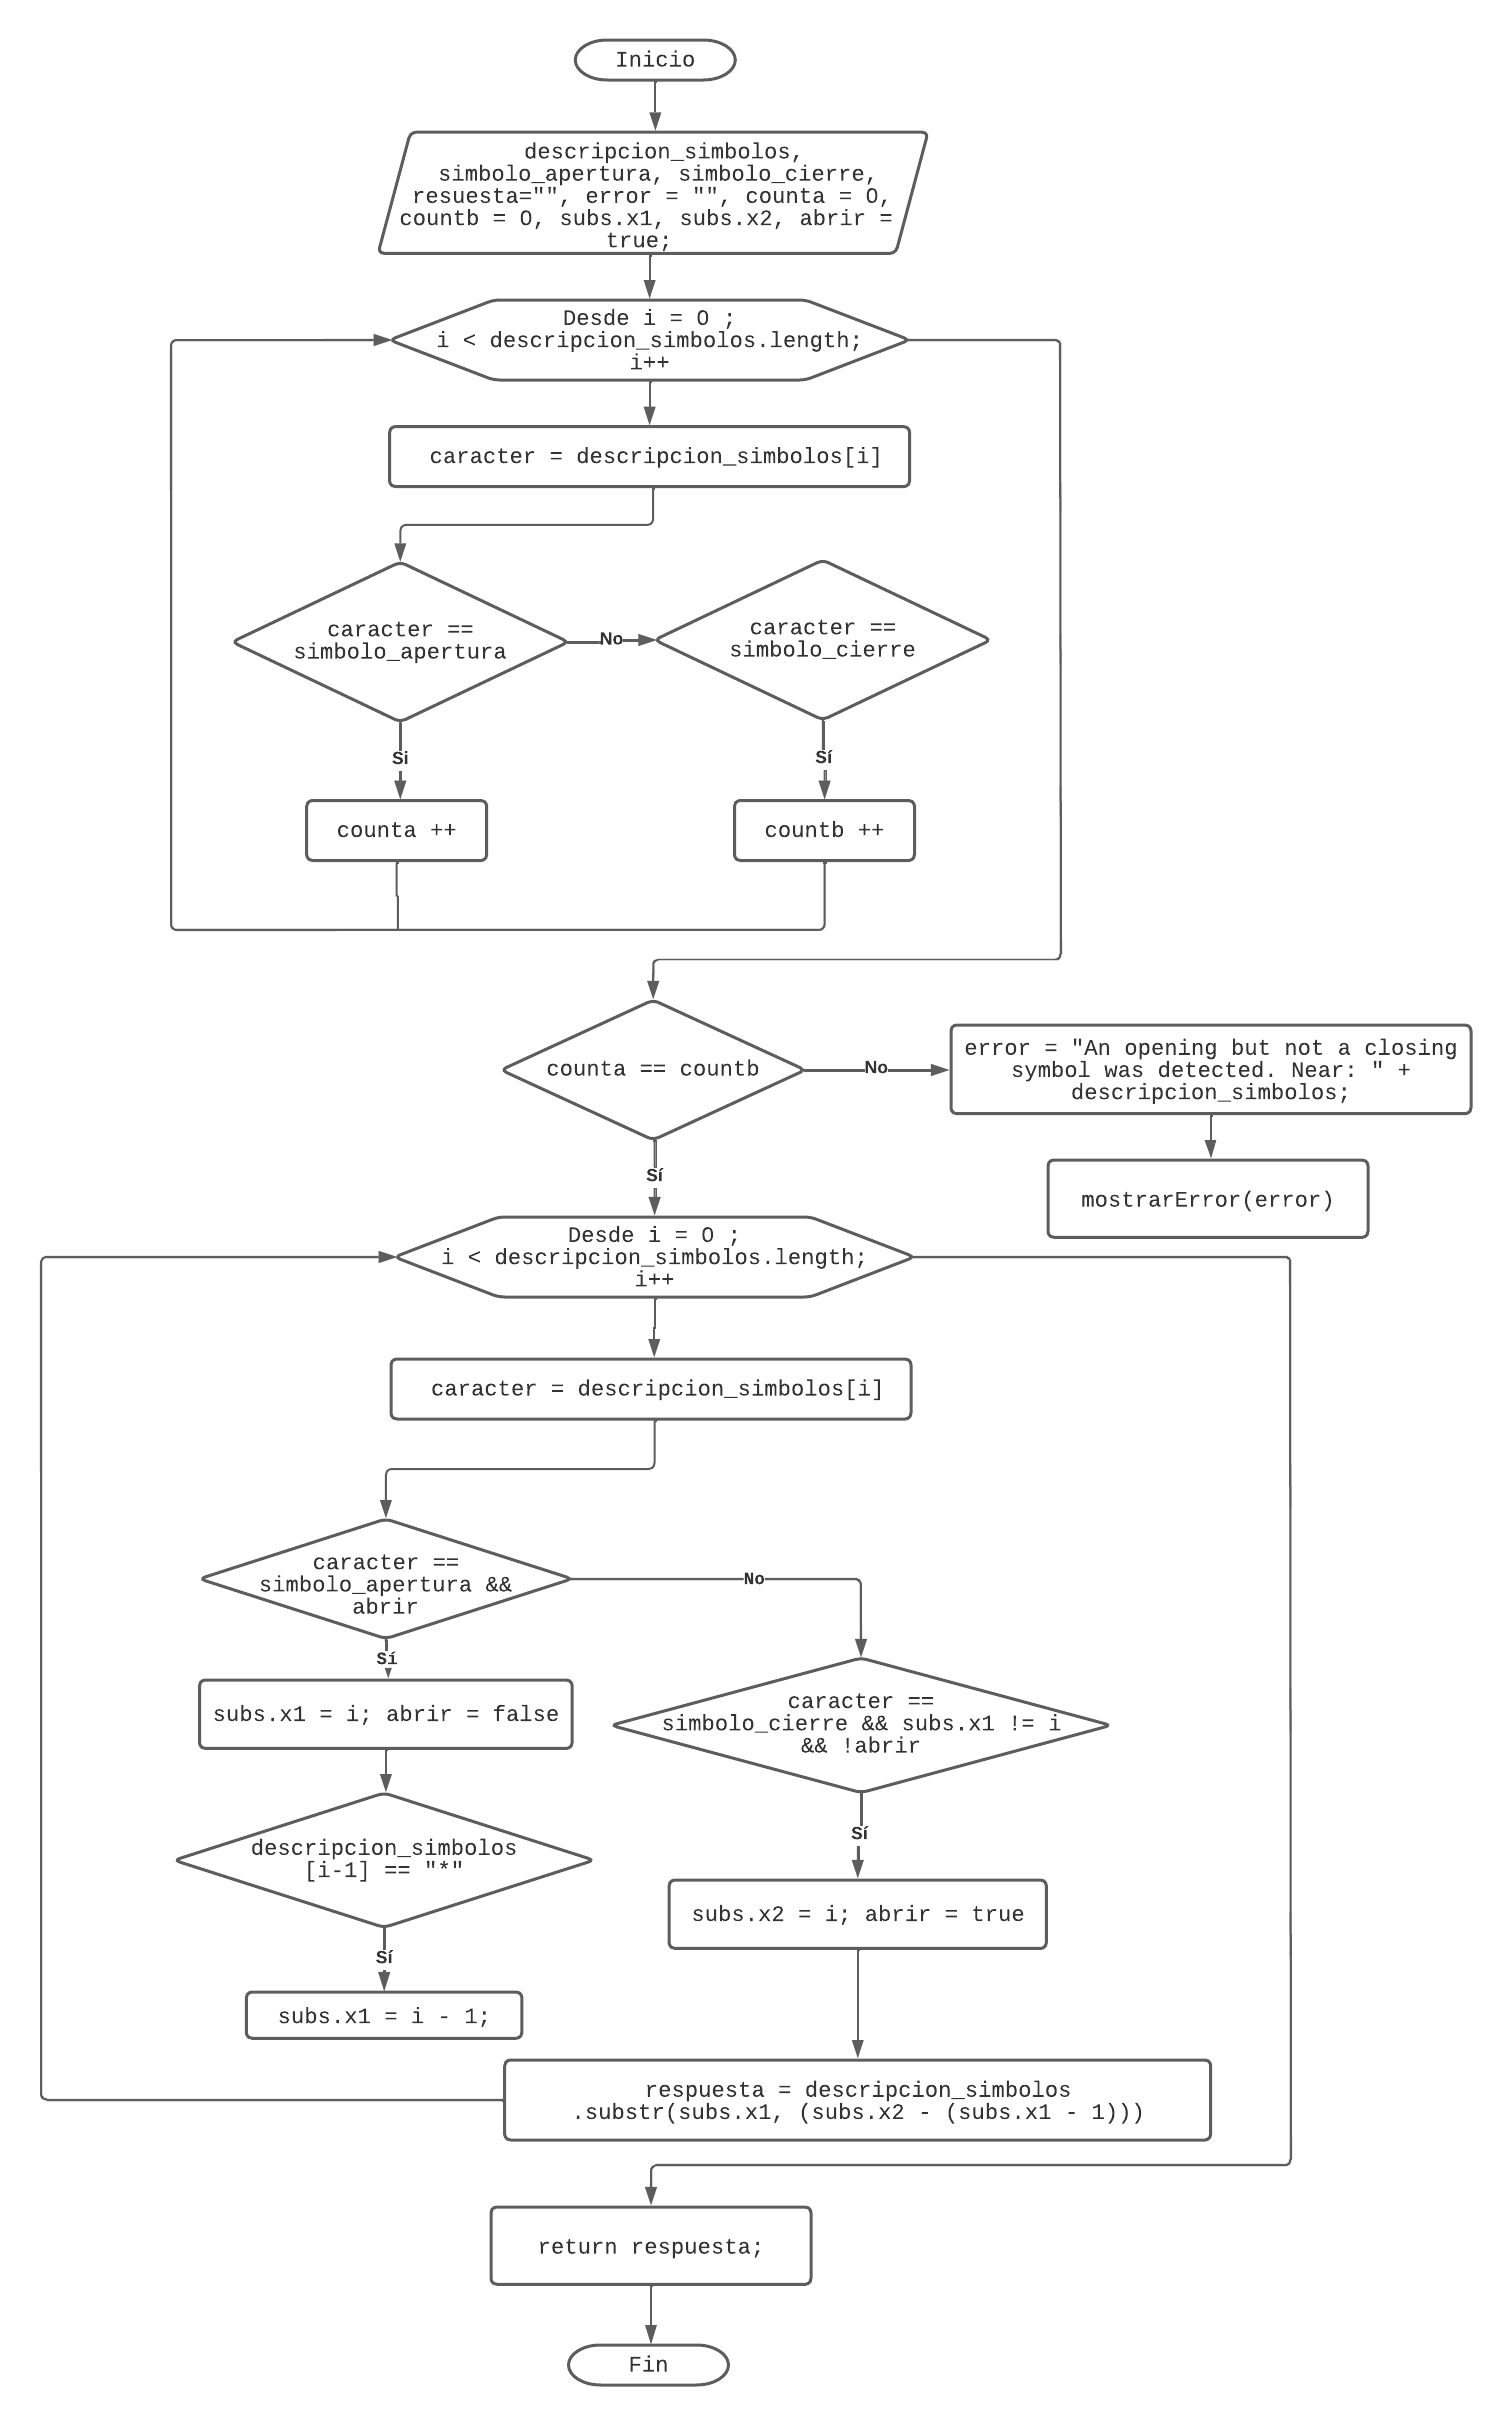
\includegraphics[width=11cm]{img/algoritmoerror.png}
	\label{fig:algoritmoerror}
	\textbf{\\ \\ ELABORADO: DÚVAL CARVAJAL SUÁREZ}
\end{figure} 

\subsection{Generación de código}

En la siguiente fase se desarrollaron las funciones y todos los métodos que fueron necesarios para que la librería funcione correctamente. A continuación, se observan todas las variables que fueron necesarias para que todo funcione de manera correcta.
\newpage
\lstinputlisting[language=JavaScript]{codigo/variables.js}

En el siguiente bloque de código se observa la función que permite acumular los mensajes de error que pueden ocurrir al momento de interpretar las descripciones de los casos de uso. 

\lstinputlisting[language=JavaScript]{codigo/notificaciones.js}

En el siguiente bloque de código se observa una de las funciones principales para detectar los símbolos de apertura y cierre, con el objetivo de utilizar una sola función que permita identificar los símbolos que necesariamente deben ser con apertura y cierre. 

\lstinputlisting[language=JavaScript]{codigo/detectarsimbolos.js}

Para mejorar la presentación de la librería se desarrolló una aplicación web sencilla que permita utilizar de forma gráfica las funciones de esta. La aplicación web tendrá como propósito proporcionar un lugar en la web de donde descargar el script para que pueda ser usado por la comunidad de desarrolladores. Además, de proporcionar documentación de como instalarla en otros proyectos y como utilizarla. 

\subsection{Ejecución de pruebas}

Para la ejecución de las pruebas, se analizó el caso de uso que fue proporcionado por el docente. Cada párrafo estaba redactado con el lenguaje de símbolos, por lo que se ingresaron las descripciones en la aplicación de demostración y los resultados fueron los siguientes:

\begin{itemize}
	\item Descripción \#1:
	\begin{lstlisting}
		This use case starts when a person *(person &-id=int) wants to register as a tutor *(tutor &-id=int [+userRegistration=Tutor]) user in the system. *¡tutor 1<[register]>n Person! \end{lstlisting}

	Interpretando el párrafo, se creó una clase denominada Tutor con sus respectivos atributos que son: \textbf{id} privado y de tipo String, los métodos que se agregaron son: \textbf{userRegistration()} público. Además, se realizó una relación de tipo generalización. A continuación, se observa la estructura json y xml generada por la librería a partir del párrafo ingresado.

\lstinputlisting[language=JavaScript]{codigo/pruebas/test01.json}
\lstinputlisting[language=JavaScript]{codigo/pruebas/test01.xml}

Para que la descripción del caso de uso pueda ser entendida por el cliente del sistema que se esté desarrollando se obtiene como resultado el párrafo redactado en lenguaje natural omitiendo los símbolos y pueda ser comprendido con mayor facilidad.

	
	\begin{lstlisting}
		This use case starts when a person wants to register as a tutor user in the system.  \end{lstlisting}
	
	Como el texto está redactado de forma correcta la retroalimentación generada muestra mensajes exitosos:
	
	\textcolor{blue}{\textbf{information:} Description entered: This use case starts when a person *(person \&-id=int) wants to register as a tutor *(tutor \&-id=int [+userRegistration=Tutor]) user in the system. *¡tutor 1<[register]>n Person!}
	
	\textcolor{ForestGreen}{
		\textbf{success:} Successfully added attributes: id \\
		\textbf{success:} The class Person was generated successfully \\
		\textbf{success:} Successfully added attributes: id \\
		\textbf{success:} The class Tutor was generated successfully \\
		\textbf{success:} The generalization relationship between objects from: Tutor 1<>n to: Person was successfully generated. }
	
	Para verificar el funcionamiento de la retroalimentación identificando la mala escritura de las descripciones del caso de uso usando el lenguaje de símbolos, se redactó a propósito el mismo párrafo usando de forma incorrecta los símbolos.
	
	\begin{lstlisting}
		This use case starts when a person *(person &-id=int) wants to register as a tutor *(tutor &-id=int [+userRegistration=Tutor) user in the system. *¡tutor 1<[register]>n Person \end{lstlisting} 
	
	Observando los menajes de retroalimentación ya se identificaron que errores se están cometiendo en el uso de algunos símbolos y especificando en qué lugar del texto se encuentra ese error.
	
	\textcolor{blue}{\textbf{information:} Description entered: This use case starts when a person *(person \&-id=int) wants to register as a tutor *(tutor \&-id=int [+userRegistration=Tutor]) user in the system. *¡tutor 1<[register]>n Person!}
	
	\textcolor{ForestGreen}{
	\textbf{success:} Successfully added attributes: id \\
	\textbf{success:} The class Person was generated successfully \\
	\textbf{success:} Successfully added attributes: id}

	\textcolor{Red}{
	\textbf{error:} An opening but not a closing symbol was detected. => begin: [, end: ]. Near: *(tutor \&-id=int [+userRegistration=Tutor)}

	\textcolor{ForestGreen}{\textbf{success:} The class Tutor was generated successfully }
	
	\textcolor{Red}{
	\textbf{error:}  An opening but not a closing symbol was detected. => begin: ¡, end: !. Near: This use case starts when a person *(person \&-id=int) wants to register as a tutor *(tutor \&-id=int [+userRegistration=Tutor) user in the system. *¡tutor 1<[register]>n Person}

	Utilizando la aplicación web de demostración, se logra observar ene la figura \ref{fig:prueba01} el diagrama de clases creado a partir de la estructura json o xml que la librería proporciona de forma automática. Para dibujar el diagrama de clases, se está utilizando la librería JavaScript jsUml2. 
	
	\begin{figure}[h!]
		\caption{Diagrama de clases generado por la aplicación web de demostración usando la librería de armadillo.js, descripción 1}
		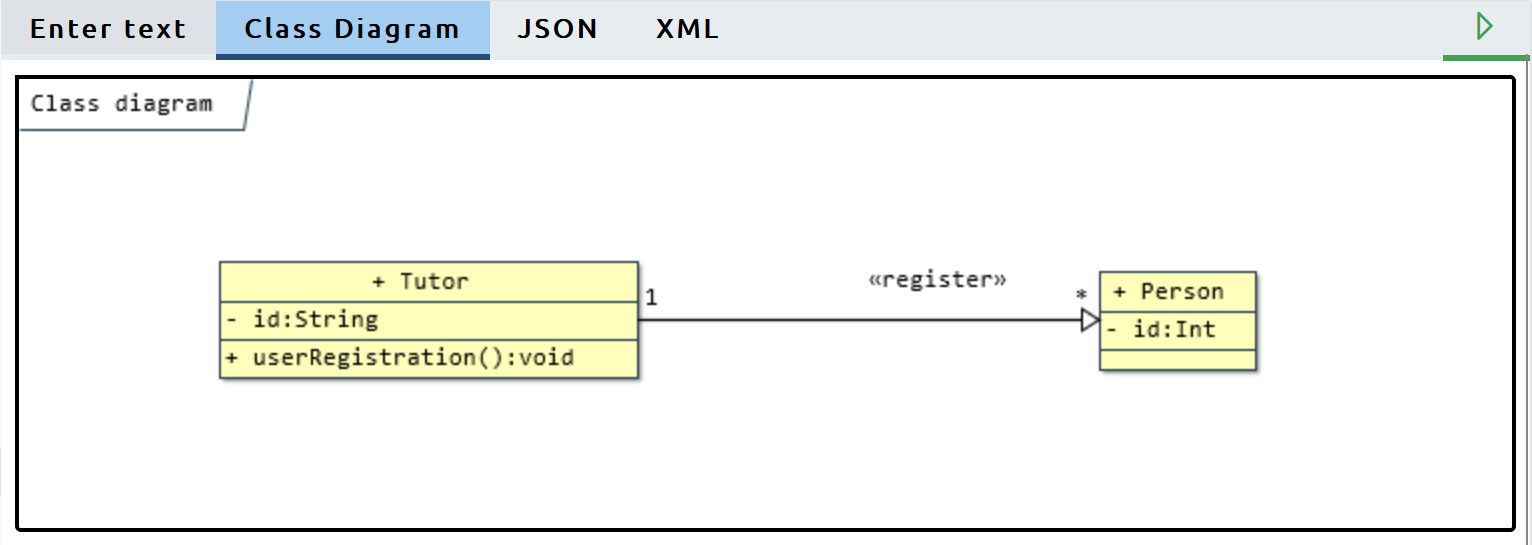
\includegraphics[width=15cm]{img/prueba01.png}
		\label{fig:prueba01}
		\textbf{\\ ELABORADO: DÚVAL CARVAJAL SUÁREZ}
	\end{figure}

	\item \textbf{Descripción \#2:}
	\begin{lstlisting}
		The person accesses then User Registration *(@User Registration) interface. *¡person1<[accesses]<1 User Registration! \end{lstlisting}

	A continuación, se evidenciará como se va modificando el diagrama de clases por cada descripción del caso de uso que se va interpretando hasta llegar al diagrama de clases final. En esta descripción se generó un nuevo objeto para el diagrama que es una interfaz denominada User Registration que se relaciona mediante dependencia a la clase Person (ver figura \ref{fig:prueba02}).
	
	\begin{lstlisting}
		The person accesses then User Registration interface. \end{lstlisting} 
	
	\begin{figure}[h!]
		\caption{Diagrama de clases generado por la aplicación web de demostración usando la librería de armadillo.js, descripción 2}
		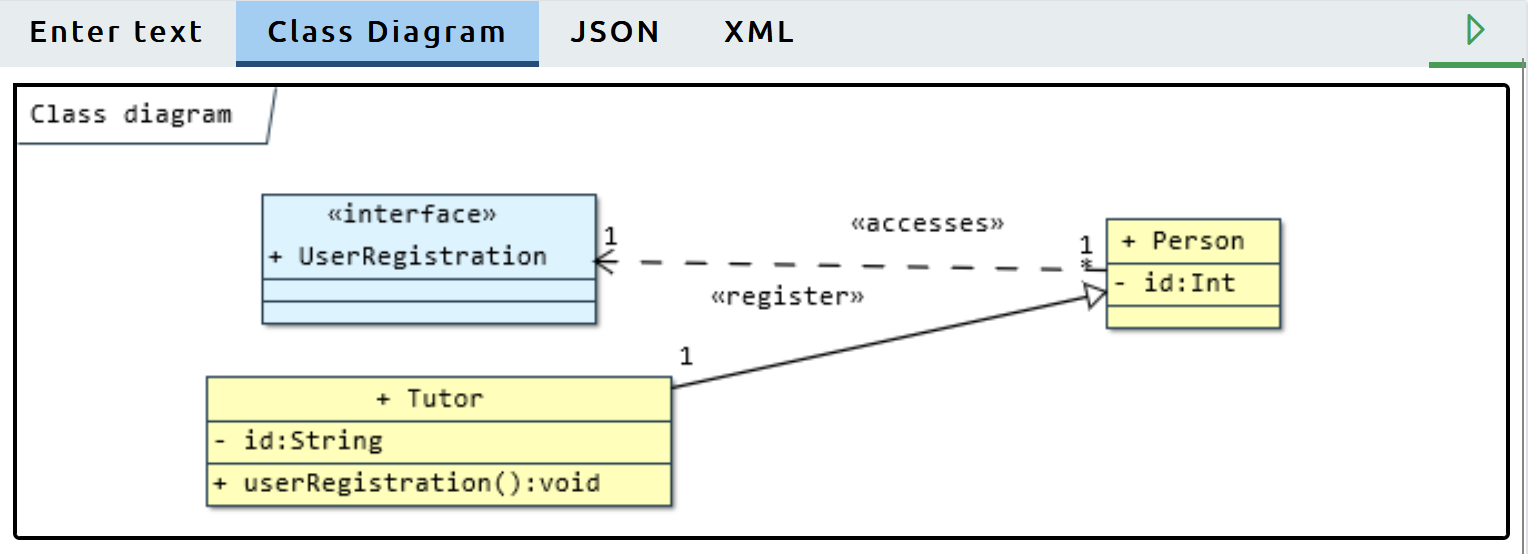
\includegraphics[width=15cm]{img/prueba02.png}
		\label{fig:prueba02}
		\textbf{\\ ELABORADO: DÚVAL CARVAJAL SUÁREZ}
	\end{figure}

	\item \textbf{Descripción \#3:}
	\begin{lstlisting}
		Shows you the fields to fill in the interface user registration *(@User registration): *(Person &-/first name/=String, &-/last name/=String, &-/date of birth/=Date, &-/gender/=String, &-/phone number/=String, &-/email/=String) *(User &-id=Int, &-/username/=String, &-/password/=String &-status=Status &-user type=UserType). It should be taken into account that the registration of a *¡/Person/ u<[/has a/]>u /User/!. There are states that can be *¿Status »/Disabled/ /o/ »/Enabled/? that each *¡/User/ u>[/will have a/]<u /Status/! . There are also several types of users, which are *¿UserType »/Tutor/ /or/ »/Patient/ /or/ »/Admin/? and every *¡/User/ u>[/will have a/]<u /UserType/!. In addition, the system assigns an id when storing it. \end{lstlisting}
	
		En esta descripción se detallaron más objetos del diagrama de clases. Se observa que se agregaron más atributos a la clase Person, se agregaron 2 objetos enum que se denominan Status y UserType, aparte que están relacionados con la clase User que también fue agregada en esta descripción.
		
		\begin{lstlisting}
		Shows you the fields to fill in the interface user registration : first name last name date of birth gender phone number email username password. It should be taken into account that the registration of a Person has a User. There are states that can be Disabled o Enabled that each User will have a Status . There are also several types of users, which are Tutor or Patient or Admin and every User will have a UserType. In addition, the system assigns an id when storing it. \end{lstlisting}

	\begin{figure}[h!]
		\caption{Diagrama de clases generado por la aplicación web de demostración usando la librería de armadillo.js, descripción 3}
		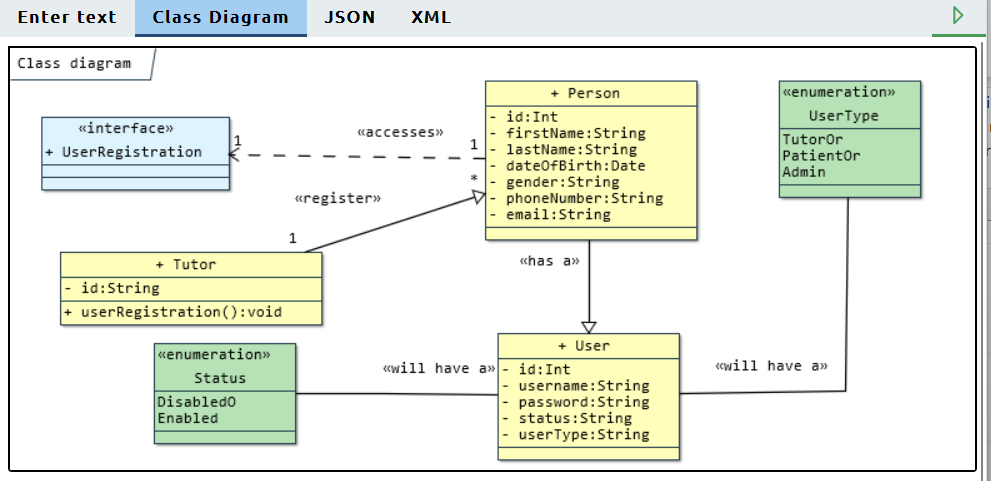
\includegraphics[width=15cm]{img/prueba03.png}
		\label{fig:prueba03}
		\textbf{\\ ELABORADO: DÚVAL CARVAJAL SUÁREZ}
	\end{figure}

	\item \textbf{Descripción \#4:}
	
	\begin{lstlisting}
		Create a *(/person/ %.first name=String, .last name=String, .date of birth=Date, .gender=String, .phone number=String, .email=String%) object \end{lstlisting}
	
	En esta descripción se agregó un nuevo constructor para la clase Person con los siguientes parámetros: firstName, lastName, dateOfBirth, gender, phoneNumber y email.
	
	\begin{lstlisting}
		Create a person object  \end{lstlisting}
	
	\begin{figure}[h!]
		\caption{Diagrama de clases generado por la aplicación web de demostración usando la librería de armadillo.js, descripción 4}
		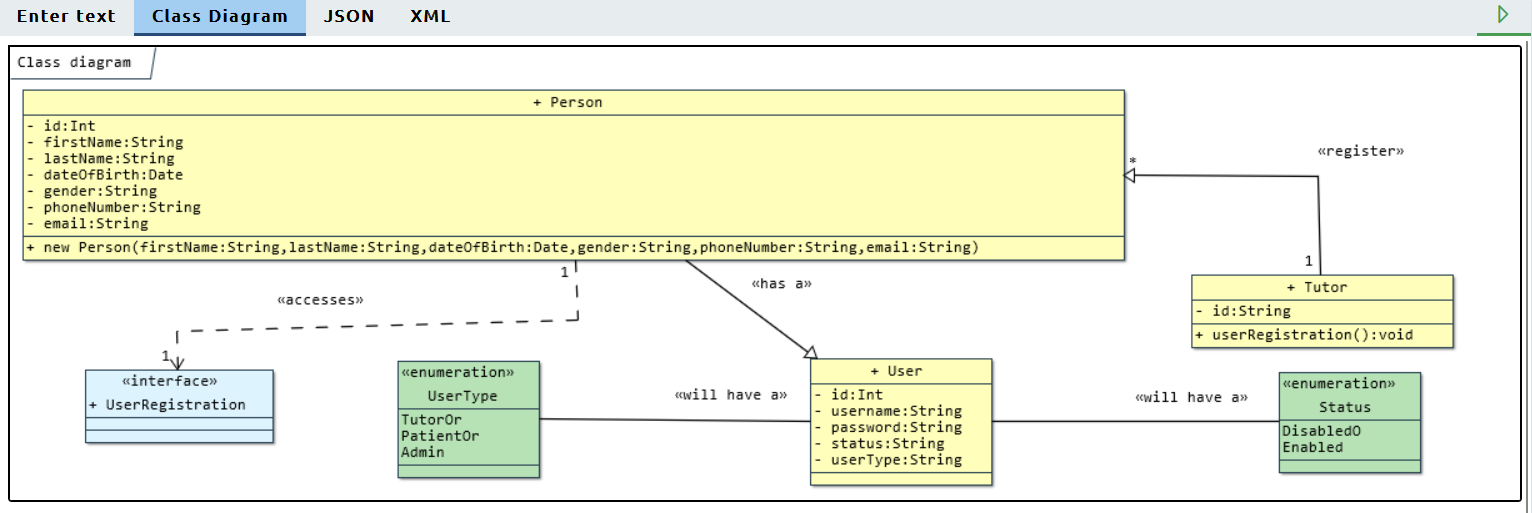
\includegraphics[width=15cm]{img/prueba04.png}
		\label{fig:prueba04}
		\textbf{\\ ELABORADO: DÚVAL CARVAJAL SUÁREZ}
	\end{figure}

	\item \textbf{Descripción \#5:}
	\begin{lstlisting}
		Create a *(/tutor/ %.person=Person%) object \end{lstlisting}

	En la siguiente descripción se agregó un nuevo constructor a la clase Tutor que recibe como parámetro un objeto de la clase Person. 
	
	\begin{lstlisting}
		Create a tutor object  \end{lstlisting}
	
	\begin{figure}[h!]
		\caption{Diagrama de clases generado por la aplicación web de demostración usando la librería de armadillo.js, descripción 5}
		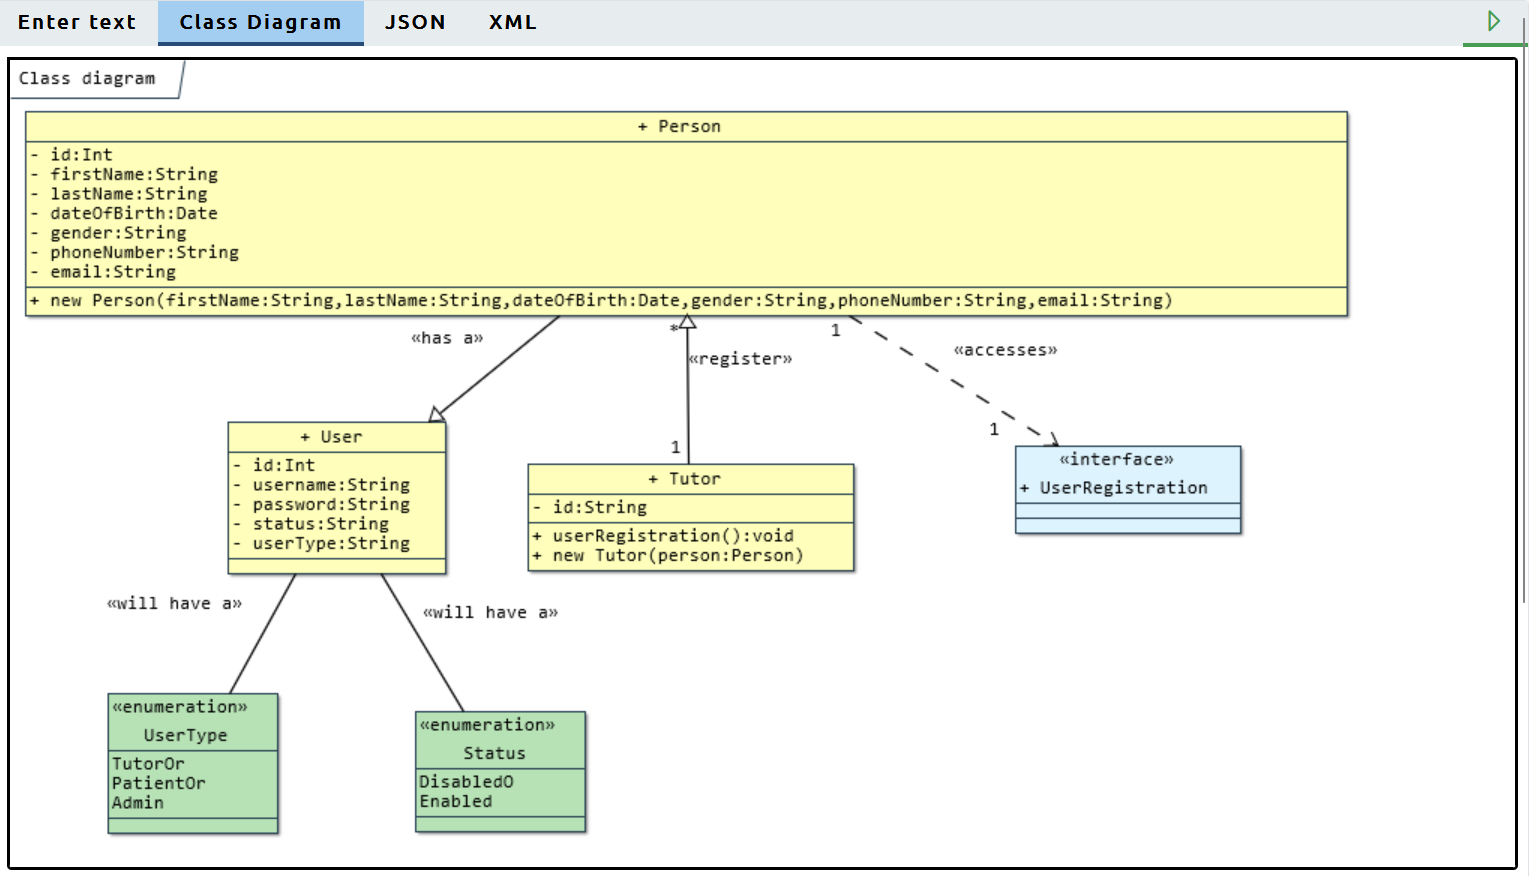
\includegraphics[width=15cm]{img/prueba05.png}
		\label{fig:prueba05}
		\textbf{\\ ELABORADO: DÚVAL CARVAJAL SUÁREZ}
	\end{figure}

	\item \textbf{Descripción \#6}
	\begin{lstlisting}
		Create an *(/user/ %.username=String, .password=String, .status=Status, .user type=UserType, .person=Tutor%) object \end{lstlisting}
	
	En la descripción se observa que se agregó un nuevo constructor a la clase User con sus parámetros que son: username, password, status, userType y person que es un objeto Tutor. 
	
	\begin{lstlisting}
		Create an user object  \end{lstlisting}
	
	\begin{figure}[h!]
		\caption{Diagrama de clases generado por la aplicación web de demostración usando la librería de armadillo.js, descripción 6}
		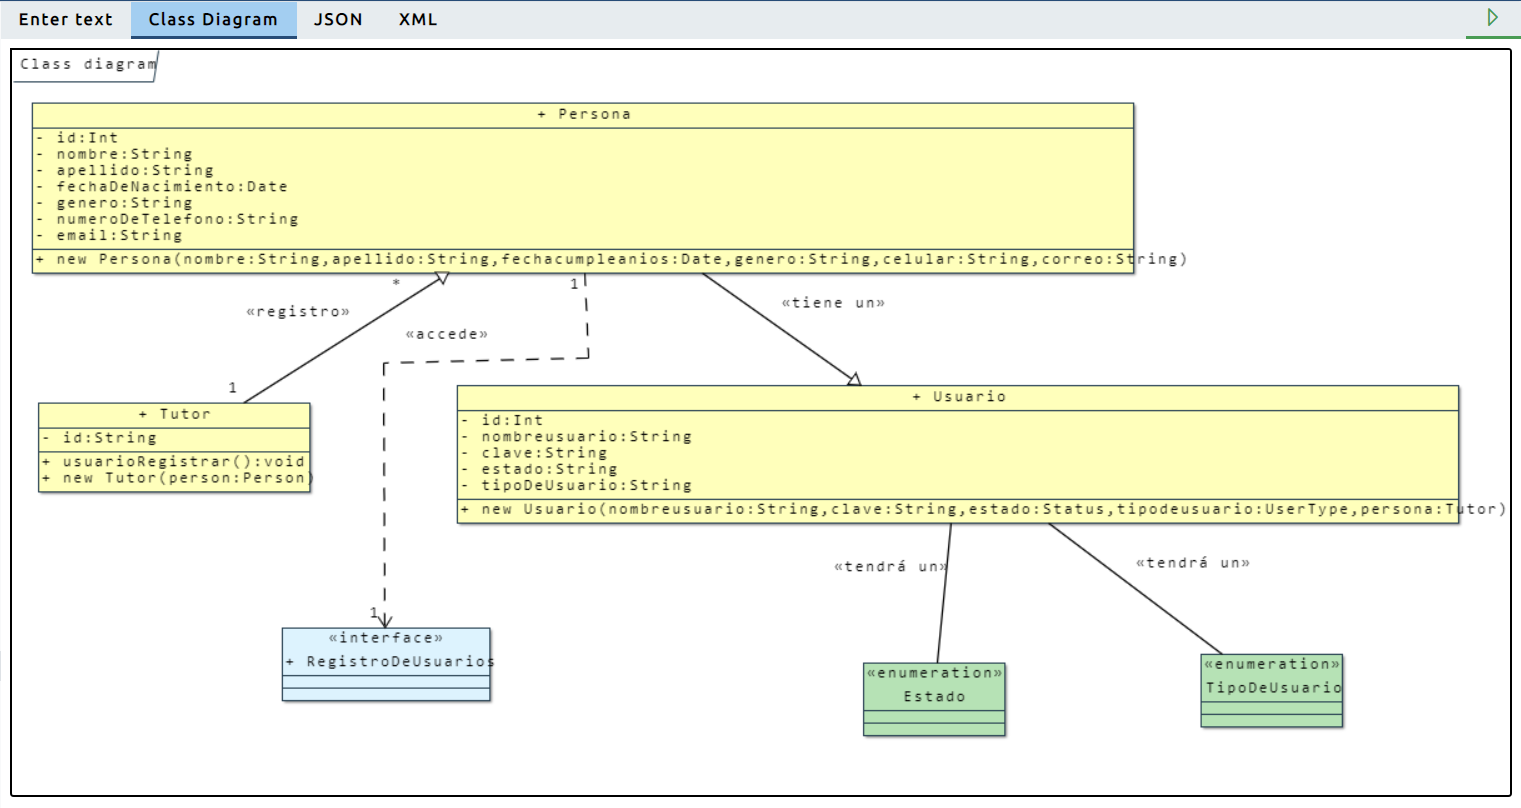
\includegraphics[width=15cm]{img/prueba06.png}
		\label{fig:prueba06}
		\textbf{\\ ELABORADO: DÚVAL CARVAJAL SUÁREZ}
	\end{figure}

	\item \textbf{Descripción \#7:}
	\begin{lstlisting}
		*(TutorDAO &id=Int [/Save/=Tutor{.tutor=Tutor}])s the tutor data in the database. *¡TutorDAO<[]< tutor! \end{lstlisting}
	
	En la siguiente descripción se observa que se agregó una nueva clase que se denomina TutorDAO. Se agregó un método que se llama Save que recibe como parámetro un objeto de tipo Tutor y retorna un objeto Tutor mismo. Además, se generó una relación de tipo Dependencia con la clase Tutor pero sin cardinalidad.
	\begin{lstlisting}
		Saves the tutor data in the database. \end{lstlisting}
	
	\begin{figure}[h!]
		\caption{Diagrama de clases generado por la aplicación web de demostración usando la librería de armadillo.js, descripción 6}
		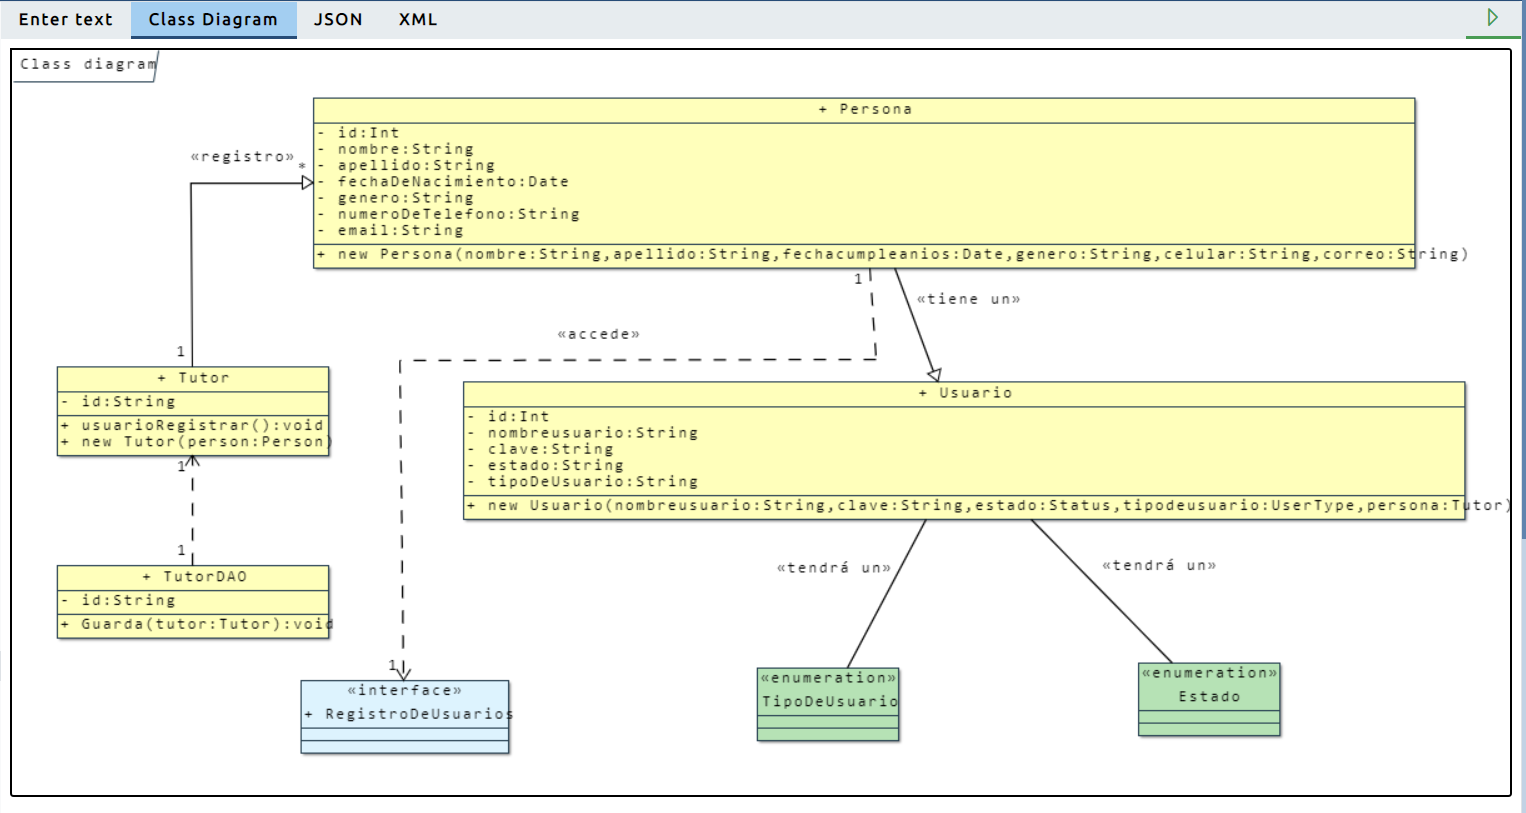
\includegraphics[width=15cm]{img/prueba07.png}
		\label{fig:prueba07}
		\textbf{\\ ELABORADO: DÚVAL CARVAJAL SUÁREZ}
	\end{figure}
	
	\item \textbf{Descripción \#8:}
	\begin{lstlisting}
	*(UserDAO &-id=Int [/Save/=User{.user=User}])s the user data in the database. *¡UserDAO <[]< User! \end{lstlisting}

	En la siguiente descripción se agregó una clase denominada UserDAO con un método llamado save que recibe como parámetro un objeto de tipo User. Además, se relaciona mediante la relación de tipo Dependencia con la clase User (ver figura \ref{fig:prueba08}).	
	
	\begin{lstlisting}
		Saves the user data in the database. \end{lstlisting}

	\begin{figure}[h!]
		\caption{Diagrama de clases generado por la aplicación web de demostración usando la librería de armadillo.js, descripción 6}
		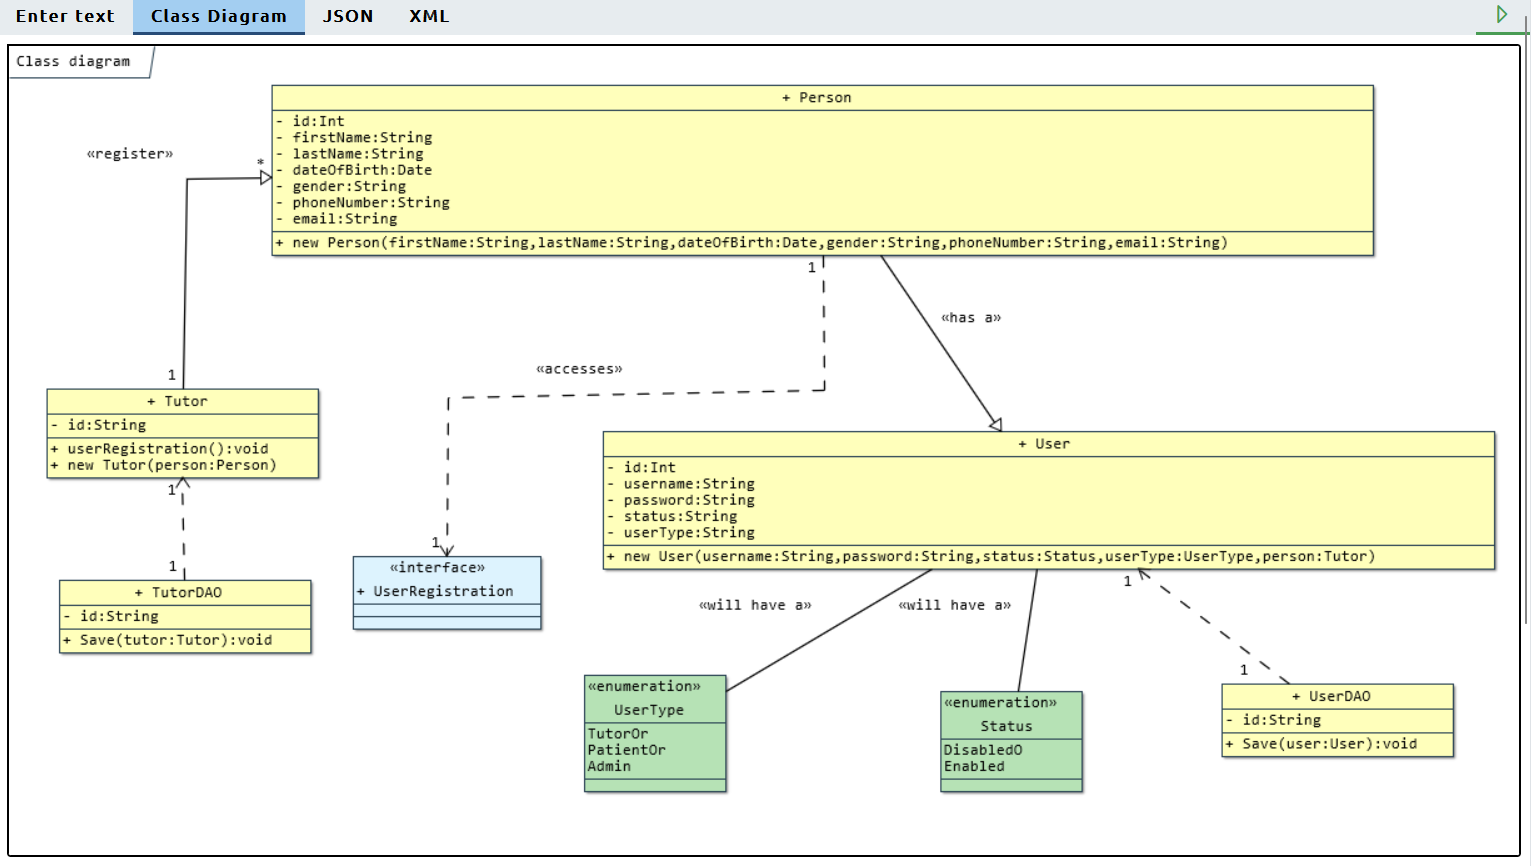
\includegraphics[width=15cm]{img/prueba08.png}
		\label{fig:prueba08}
		\textbf{\\ ELABORADO: DÚVAL CARVAJAL SUÁREZ}
	\end{figure}

	\item \textbf{Descripción \#9:}
	\begin{lstlisting}
		This use case ends when the system displays the *(@Login) login Interface. *¡Login u<[]<u UserDAO! \end{lstlisting}
	
	Finalmente, la descripción del caso de uso genera una interfaz que se denomina Login. Además está relacionada por medio del tipo Dependencia con la clase UserDAO (ver figura \ref{fig:prueba09}).
	
	\begin{lstlisting}
		This use case ends when the system displays the login Interface. \end{lstlisting}
	
	\begin{figure}[h!]
		\caption{Diagrama de clases generado por la aplicación web de demostración usando la librería de armadillo.js, descripción 6}
		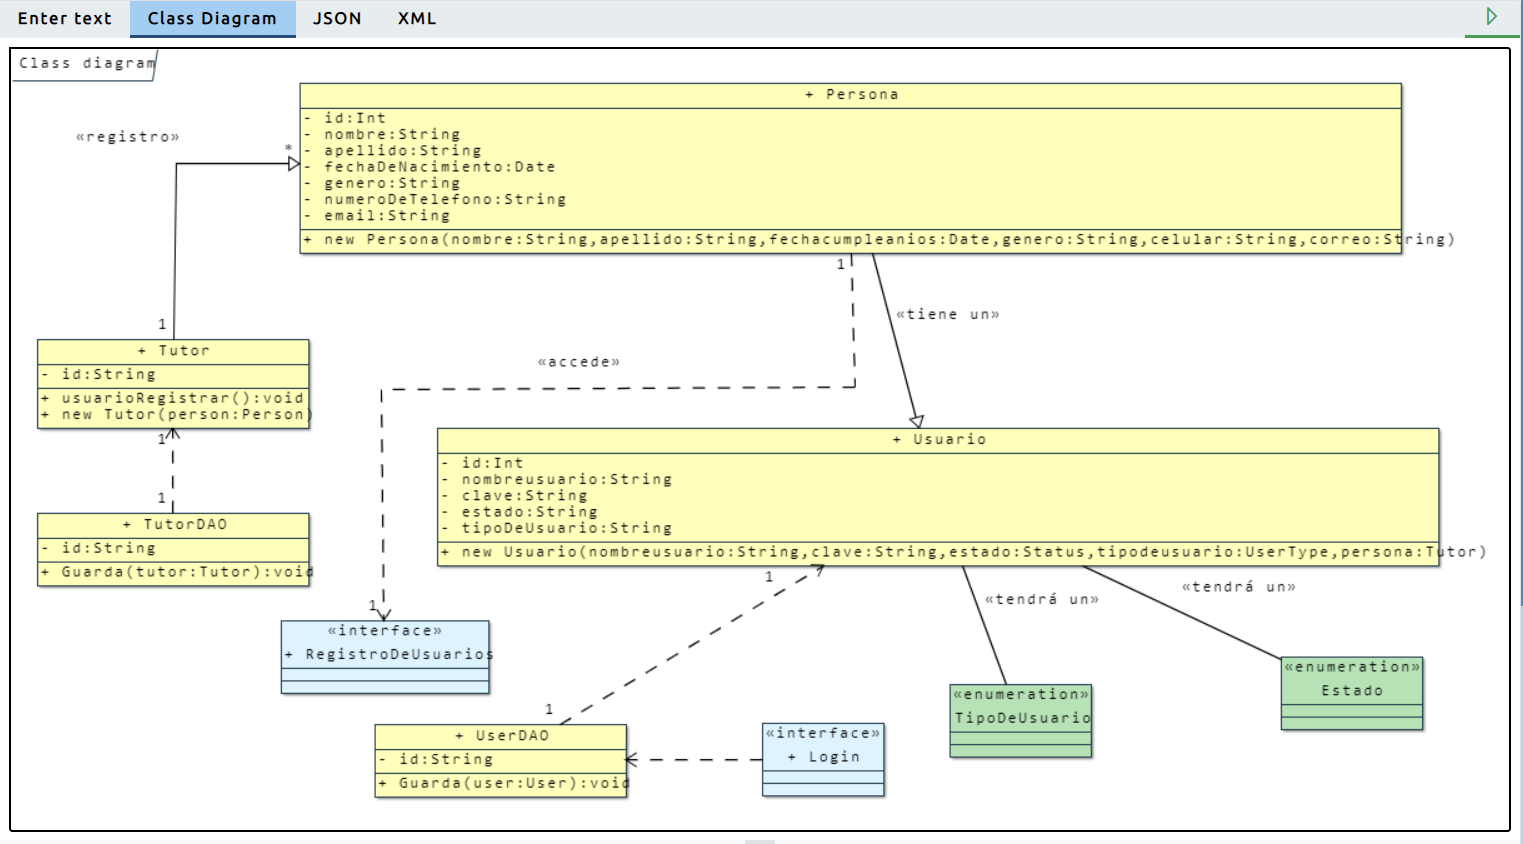
\includegraphics[width=15cm]{img/prueba09.png}
		\label{fig:prueba09}
		\textbf{\\ ELABORADO: DÚVAL CARVAJAL SUÁREZ}
	\end{figure}
	
\end{itemize}

Si se compara el diagrama de clases que fue recopilado en la primera fase de la metodología con el diagrama de clases generado mediante la librería. Se logra observar que son muy similares, y fue generado mediante las descripciones del caso de uso que fueron redactadas usando el lenguaje de símbolos.

\subsection{Evaluación con sistemas de información}

Para la ejecución de la fase final de la metodología se revisaron varios proyectos de titulación realizados por estudiantes de la Universidad Técnica Estatal de Quevedo. Se analizaron los sistemas desarrollados reescribiendo las descripciones de los casos de uso utilizando el lenguaje de símbolos.

En \cite{Villafuerte2020} se analizó el proyecto de titulación "SISTEMA BASADO EN INTERNET DE LAS COSAS PARA LA GESTIÓN DE LOS RECURSOS DE UN AULA DE CLASES" que fue realizado en la Universidad Técnica Estatal de Quevedo. Para empezar con el análisis se revisó el diagrama de casos de uso, seleccionando algunos casos de uso para realizar la respectiva evaluación de la librería. 

El objetivo de esta prueba es retroalimentar lo que se genera al interpretar cada descripción y comparar el diagrama de clases generado con el original del proyecto. En la figura \ref{fig:dcu_aula_inteligente} se observa el diagrama de casos de uso realizado por el proyecto de titulación. Para la evaluación se seleccionaron los casos: ingresar al sistema, solicitar accesos físicos temporales, acceder a cursos temporales, registrar asistencia de estudiantes.

\begin{figure}[h!]
	\caption{Diagrama de casos de uso para "SISTEMA BASADO EN INTERNET DE LAS COSAS PARA LA GESTIÓN DE LOS RECURSOS DE UN AULA DE CLASES"}
	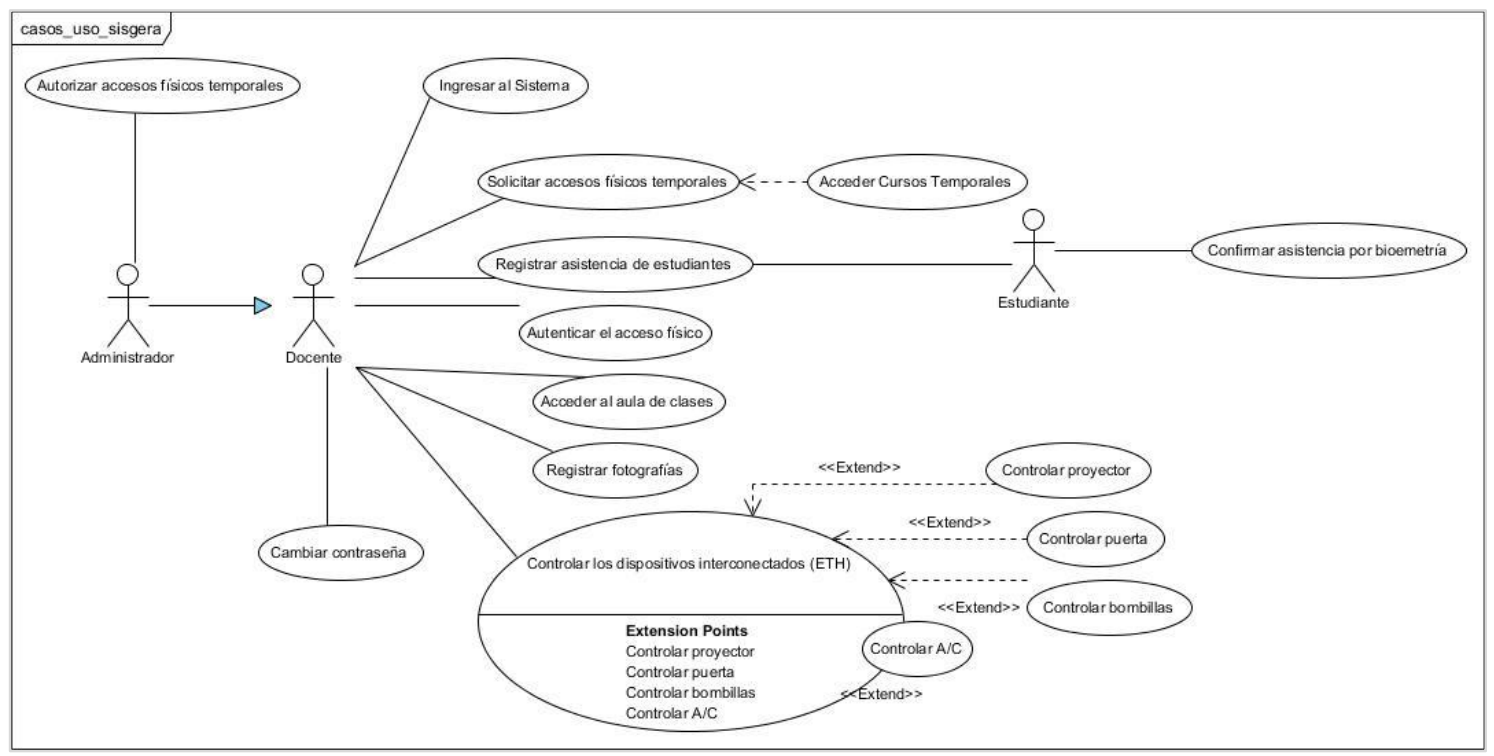
\includegraphics[width=13cm]{img/dgcu-aula-int.png}
	\label{fig:dcu_aula_inteligente}
	\textbf{\\ ELABORADO: Villafuerte y Yánez}
\end{figure}

Para mejorar la presentación de los casos de uso a evaluar, se realizó un diagrama de casos de uso con los seleccionados. Además, se redactaron las descripciones de cada caso de uso en 2 formas. La primera es con el texto natural detallando paso a paso las acciones que se deben realizar. La Segunda forma en como están representados los casos de uso es mediante el lenguaje de símbolos.

\begin{figure}[h!]
	\caption{Diagrama de casos de uso basado en el "SISTEMA BASADO EN INTERNET DE LAS COSAS PARA LA GESTIÓN DE LOS RECURSOS DE UN AULA DE CLASES" para ser evaluado por armadillo.js}
	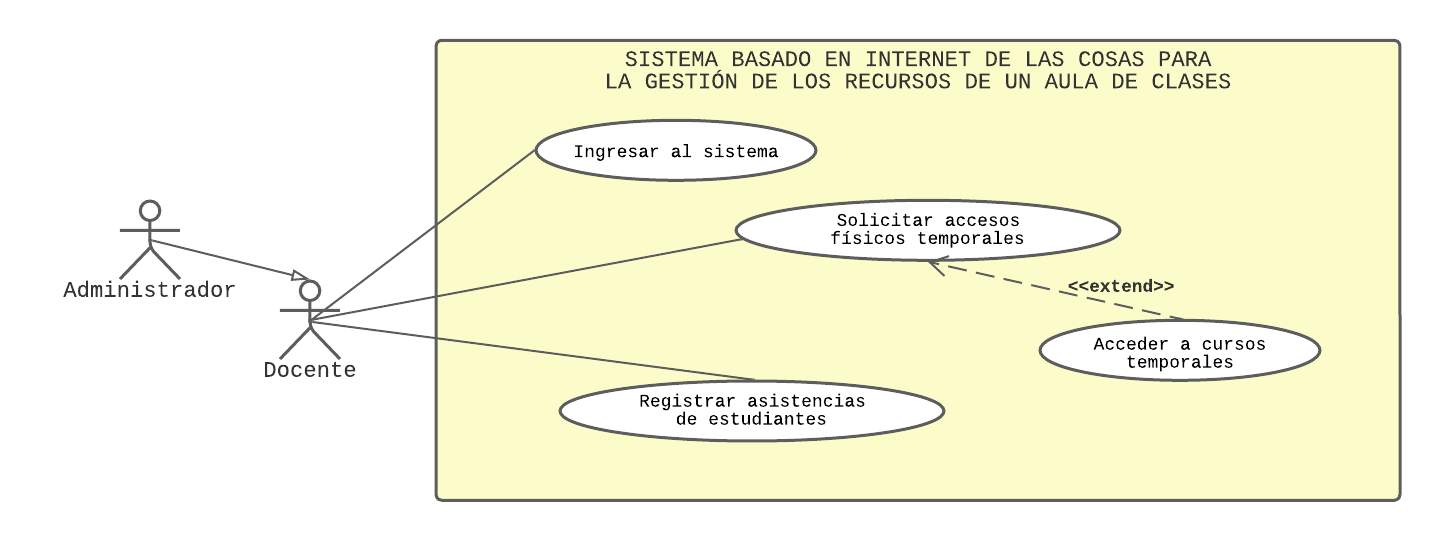
\includegraphics[width=15cm]{img/dcu_eva_ai.png}
	\label{fig:dcu_eva_aula_inteligente}
	\textbf{\\ ELABORADO: DÚVAL CARVAJAL SUÁREZ}
\end{figure}

\begin{figure}[h!]
	\caption{Diagrama de clases de el "SISTEMA BASADO EN INTERNET DE LAS COSAS PARA LA GESTIÓN DE LOS RECURSOS DE UN AULA DE CLASES" para ser evaluado por armadillo.js}
	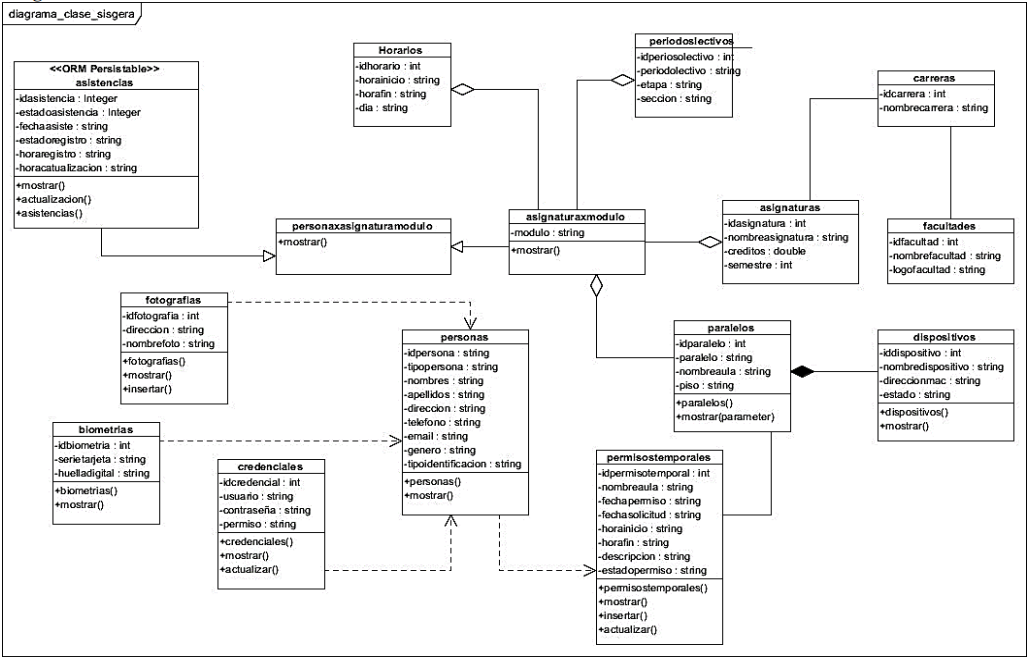
\includegraphics[width=13cm]{img/dclases-ai.png}
	\label{fig:dc_aula_inteligente}
	\textbf{\\ ELABORADO: DÚVAL CARVAJAL SUÁREZ}
\end{figure}

En la figura \ref{fig:dc_aula_inteligente} se observa el diagrama de clases para el sistema de información a analizar. En la fase de evaluación de la librería se tratará de generar un diagrama de clases lo más parecido posible al diagrama original. Además de indicar los errores si es que son cometidos al momento de redactar las descripciones de los casos de uso. 

A continuación en las tablas [\ref{tab:is_ai}, \ref{tab:sa_ai}, \ref{tab:ac_ai} \ref{tab:rae_ai}] se redactan las descripciones de los casos de uso seleccionados en lenguaje natural. En las tablas [\ref{tab:is_is_ls}, \ref{tab:aft_ai_ls}, \ref{tab:ac_ai_ls}, \ref{tab:rae_ai_ls}] se redactaron las descripciones de los casos de uso usando el lenguaje de símbolos.

Para evaluar las descripciones de los casos de uso se detallará cada descripción con su respectiva retroalimentación y como se va modificando el diagrama de clases conforme se ingresan más descripciones.

\begin{lstlisting}[]
	1. El actor docente o administrador *(persona) ingresará las *(credenciales) credenciales proporcionadas por la institución, estas se validarán y posterior otorgará el acceso a las opciones. \end{lstlisting}

\begin{figure}[h!]
	\caption{Mensajes de consola notificando si existe algún error en la escritura de la descripción 1.}
	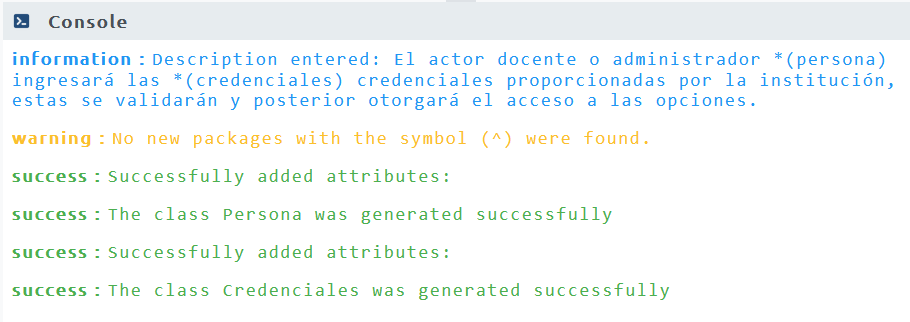
\includegraphics[width=12cm]{img/not-eva-001.png}
	\label{fig:not_eva_001}
	\textbf{\\ ELABORADO: DÚVAL CARVAJAL SUÁREZ}
\end{figure}

\begin{figure}[H]
	\caption{Diagrama de clases generado para la descripción 1.}
	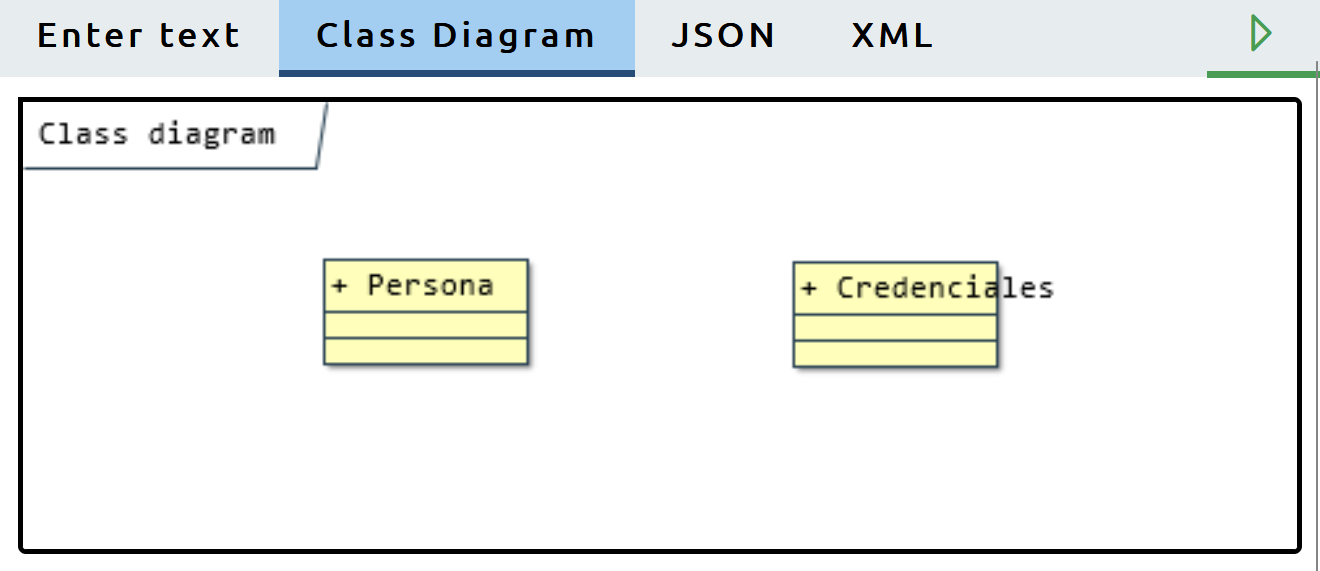
\includegraphics[width=10cm]{img/dc-eva-001.png}
	\label{fig:dc_eva_001}
	\textbf{\\ ELABORADO: DÚVAL CARVAJAL SUÁREZ}
\end{figure}

\begin{lstlisting}
	 2. El caso de uso se inicia cuando el actor docente o administrador *(persona &-id=string &-tipo=string &-nombres=string &-apellidos=string &-direccion=string &-telefono=string &-email=string &-genero = string &-tipoidentificion=string [+persona=empty] [+mostrar=empty]) necesita acceder a la aplicación, para ello ingresa a la aplicación móvil en su dispositivo smartphone. \end{lstlisting}
 
 \begin{figure}[h!]
 	\caption{Mensajes de consola notificando si existe algún error en la escritura de la descripción 2.}
 	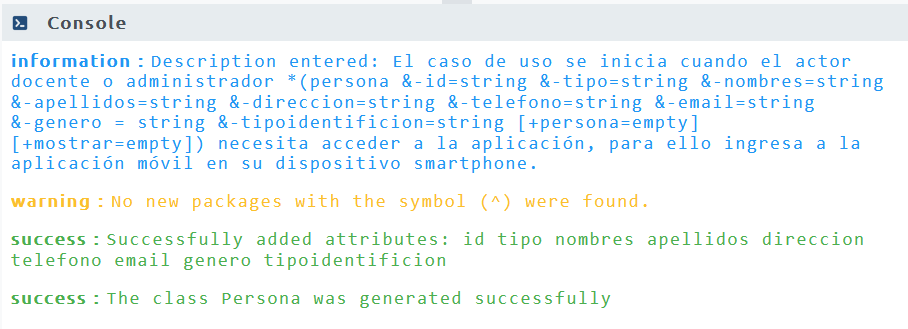
\includegraphics[width=14cm]{img/not-eva-002.png}
 	\label{fig:not_eva_002}
 	\textbf{\\ ELABORADO: DÚVAL CARVAJAL SUÁREZ}
 \end{figure}
 
 \begin{figure}[H]
 	\caption{Diagrama de clases generado para la descripción 2.}
 	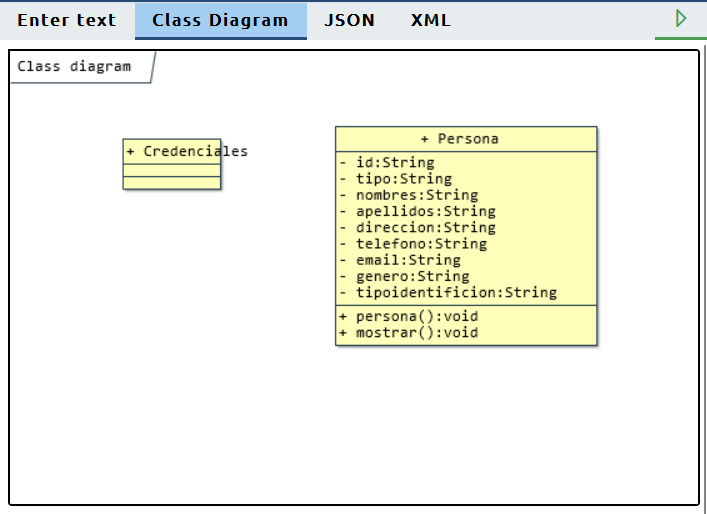
\includegraphics[width=10cm]{img/dc-eva-002.png}
 	\label{fig:dc_eva_002}
 	\textbf{\\ ELABORADO: DÚVAL CARVAJAL SUÁREZ}
 \end{figure}
 
 \begin{lstlisting}
 	3. El actor docente o administrador ingresa el *(credenciales &-id=int &-/usuario/=String /y/ &-/contraseña/=String &-permiso=string [+credenciales=empyt] [+mostrar=empty] [+actualizar=empty]) asignados por la institución; y da clic en el botón Ingresar. *¡persona 1<[tiene]<1 credenciales! \end{lstlisting}
 
  \begin{figure}[h!]
 	\caption{Mensajes de consola notificando si existe algún error en la escritura de la descripción 3.}
 	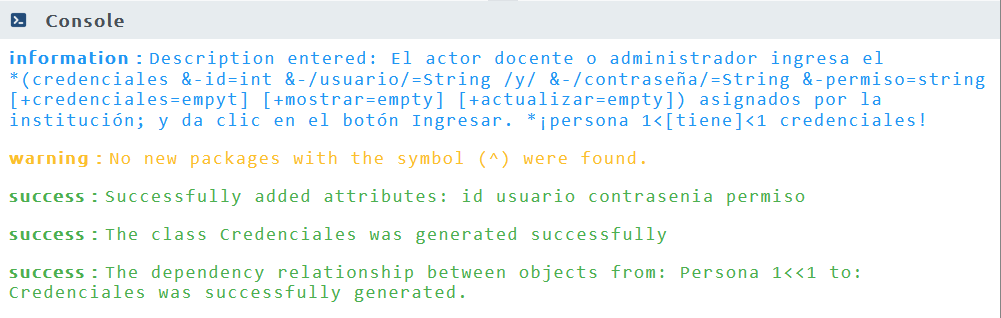
\includegraphics[width=14cm]{img/not-eva-003.png}
 	\label{fig:not_eva_003}
 	\textbf{\\ ELABORADO: DÚVAL CARVAJAL SUÁREZ}
 \end{figure}
 
 \begin{figure}[H]
 	\caption{Diagrama de clases generado para la descripción 3.}
 	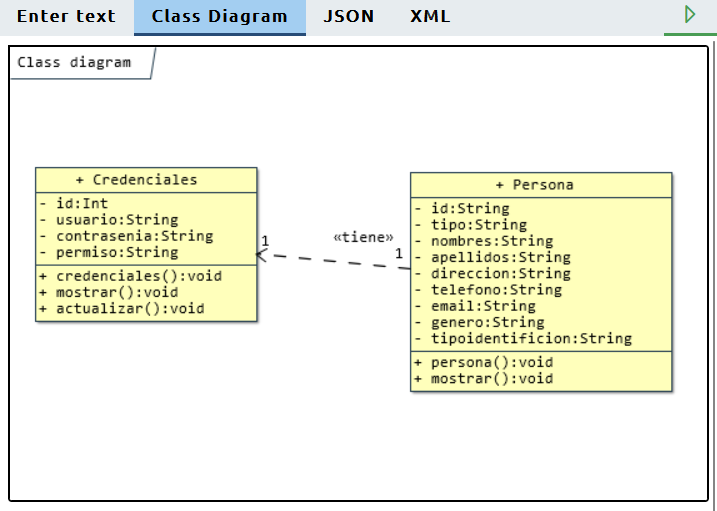
\includegraphics[width=10cm]{img/dc-eva-003.png}
 	\label{fig:dc_eva_003}
 	\textbf{\\ ELABORADO: DÚVAL CARVAJAL SUÁREZ}
 \end{figure}
 
  \begin{lstlisting}
 	4. El caso de uso se inicia cuando el docente necesita tener acceso temporalmente *(permisos temporales [+permisosTemporales=empyt] [+mostrar=empty] [+insertar=empty] [+actualizar=empty]) a un aula de clases que se encuentre disponible no utilizada. \end{lstlisting}
 
   \begin{figure}[h!]
 	\caption{Mensajes de consola notificando si existe algún error en la escritura de la descripción 4.}
 	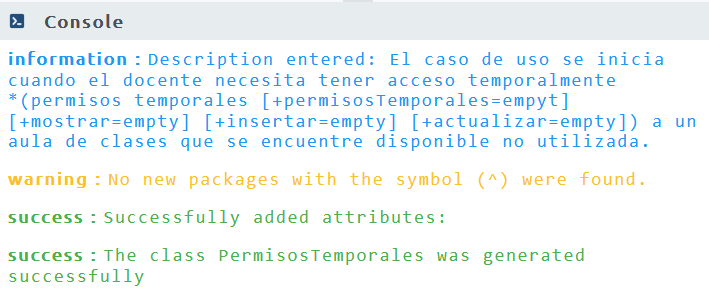
\includegraphics[width=14cm]{img/not-eva-004.png}
 	\label{fig:not_eva_004}
 	\textbf{\\ ELABORADO: DÚVAL CARVAJAL SUÁREZ}
 \end{figure}
 
 \begin{figure}[H]
 	\caption{Diagrama de clases generado para la descripción 4.}
 	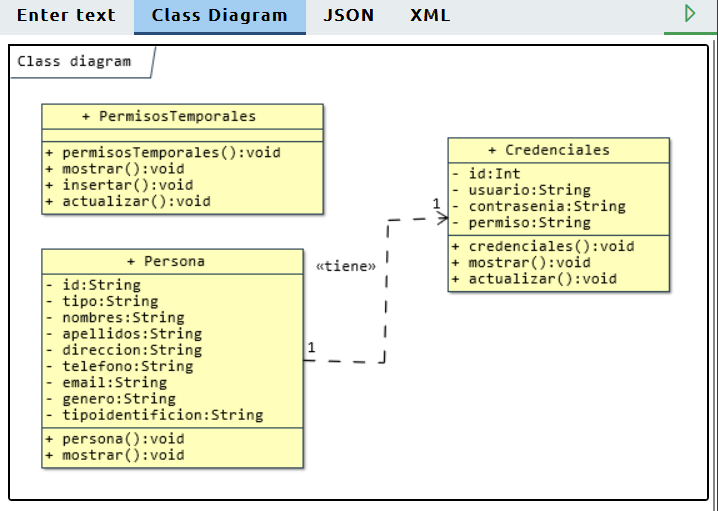
\includegraphics[width=10cm]{img/dc-eva-004.png}
 	\label{fig:dc_eva_004}
 	\textbf{\\ ELABORADO: DÚVAL CARVAJAL SUÁREZ}
 \end{figure}
 
 \begin{lstlisting}
 	5. El docente llenará la información solicitada por la interfaz, que consiste en el curso a solicitar, la *(permisos temporales &-id=int &-nombreaula &-/fecha del permiso/=string /que requiere el acceso,/ &-fecha de la solicitud=string &-/hora de inicio/=string /y/ &-/hora de fin/=string /del permiso; y, una/ &-/descripción/=string &-estado=string) donde detallará brevemente la justificación del permiso. Una vez culminado, dará clic en el botón Enviar. *¡persona 1<[podra solicitar]<1 permisos temporales! \end{lstlisting}
 
    \begin{figure}[h!]
 	\caption{Mensajes de consola notificando si existe algún error en la escritura de la descripción 5.}
 	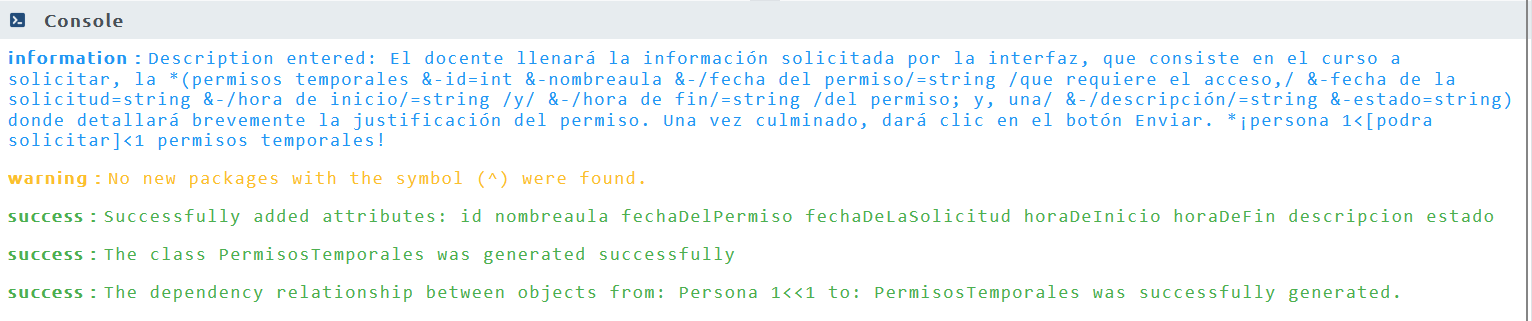
\includegraphics[width=15cm]{img/not-eva-005.png}
 	\label{fig:not_eva_005}
 	\textbf{\\ ELABORADO: DÚVAL CARVAJAL SUÁREZ}
 \end{figure}
 
 \begin{figure}[H]
 	\caption{Diagrama de clases generado para la descripción 5.}
 	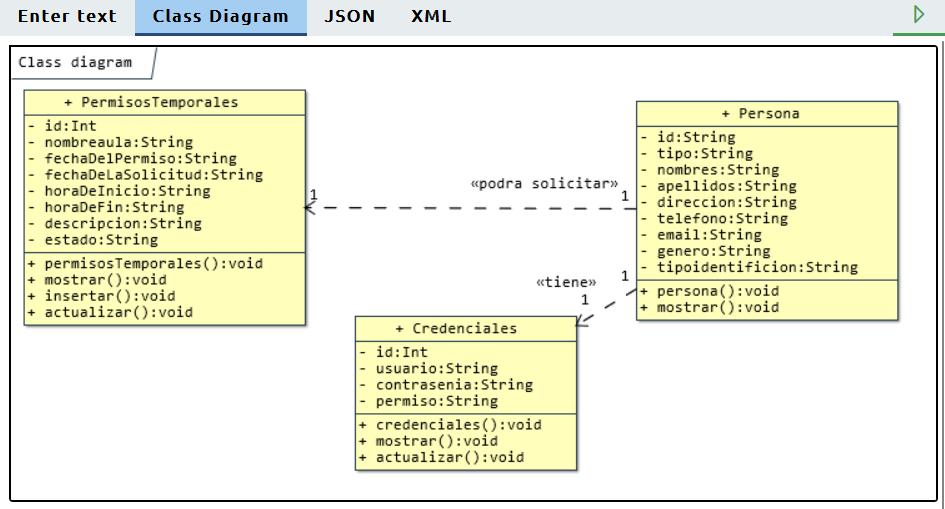
\includegraphics[width=15cm]{img/dc-eva-005.png}
 	\label{fig:dc_eva_005}
 	\textbf{\\ ELABORADO: DÚVAL CARVAJAL SUÁREZ}
 \end{figure}
 
 \begin{lstlisting}
 	6. Ingresar al aula de clases *(paralelos &-id=int &-paralelo=string &-nombreaula=string &-piso=string [+paralelos=empty] [+mostrar=empty]) que el docente solicitó un permiso temporal, previo a la autorización del administrador \end{lstlisting}
 
    \begin{figure}[h!]
 	\caption{Mensajes de consola notificando si existe algún error en la escritura de la descripción 6.}
 	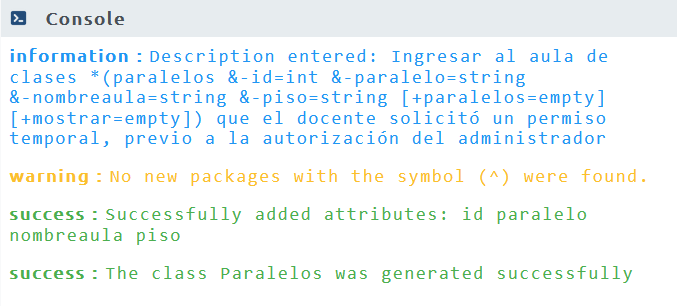
\includegraphics[width=10cm]{img/not-eva-006.png}
 	\label{fig:not_eva_006}
 	\textbf{\\ ELABORADO: DÚVAL CARVAJAL SUÁREZ}
 \end{figure}
 
 \begin{figure}[H]
 	\caption{Diagrama de clases generado para la descripción 6.}
 	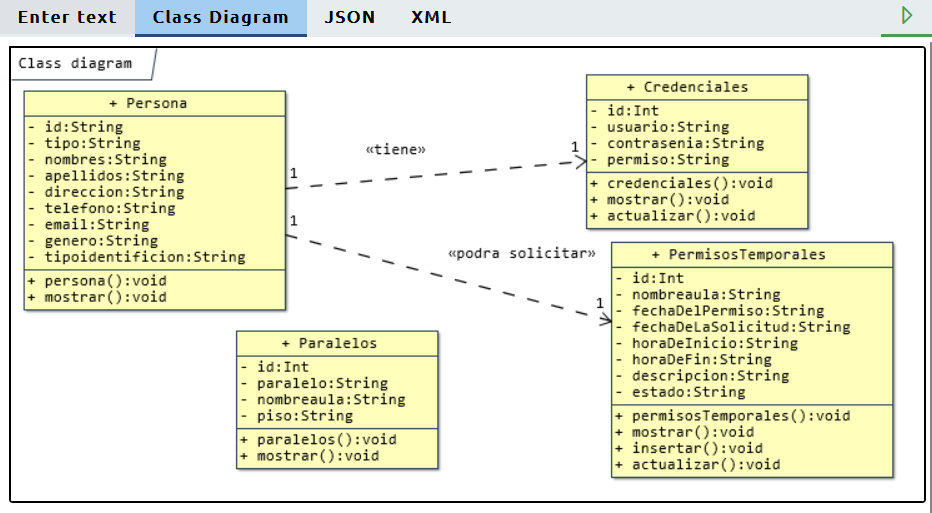
\includegraphics[width=15cm]{img/dc-eva-006.png}
 	\label{fig:dc_eva_006}
 	\textbf{\\ ELABORADO: DÚVAL CARVAJAL SUÁREZ}
 \end{figure}
 
  \begin{lstlisting}
 	7. Acceso al curso temporal en la aplicación móvi  luego de obtener autorización, donde podrá manipular los dispositivos *(dispositivos &-id=int &-nombre=string &-direccionmac &-estado=string [+dispositivos=empty] [+mostrar=empty]) eléctricos y electrónicos ETH. \end{lstlisting}
 
     \begin{figure}[h!]
 	\caption{Mensajes de consola notificando si existe algún error en la escritura de la descripción 7.}
 	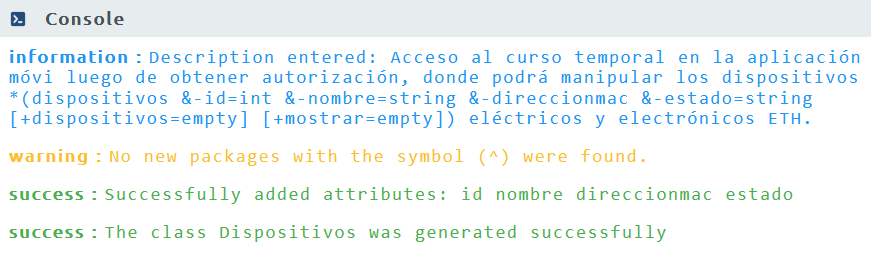
\includegraphics[width=14cm]{img/not-eva-007.png}
 	\label{fig:not_eva_007}
 	\textbf{\\ ELABORADO: DÚVAL CARVAJAL SUÁREZ}
 \end{figure}
 
 \begin{figure}[H]
 	\caption{Diagrama de clases generado para la descripción 7.}
 	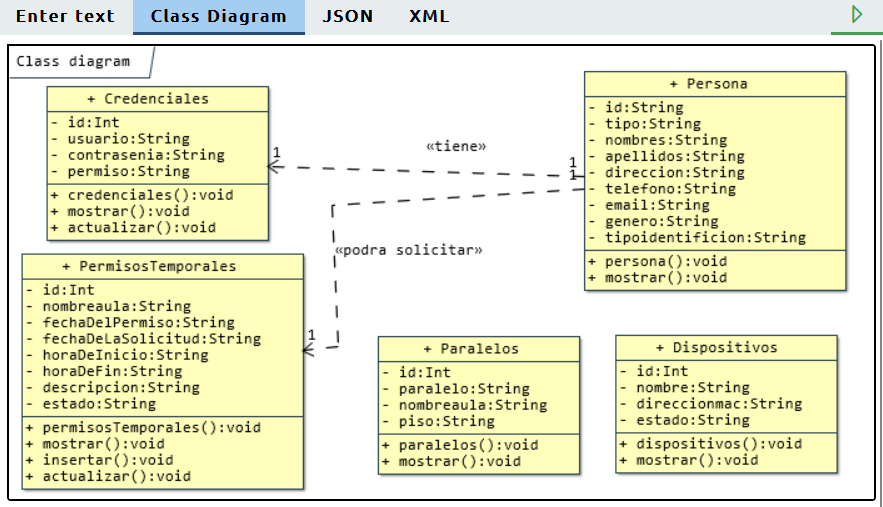
\includegraphics[width=15cm]{img/dc-eva-007.png}
 	\label{fig:dc_eva_007}
 	\textbf{\\ ELABORADO: DÚVAL CARVAJAL SUÁREZ}
 \end{figure}
 
 \begin{lstlisting}
 	8. El caso de uso se inicia cuando el docente *¡permisos temporales 1<[/accede temporalmente/]>n paralelos! a un aula de clases que se encuentre disponible, es decir no utilizada.
 \end{lstlisting}

     \begin{figure}[h!]
	\caption{Mensajes de consola notificando si existe algún error en la escritura de la descripción 8.}
	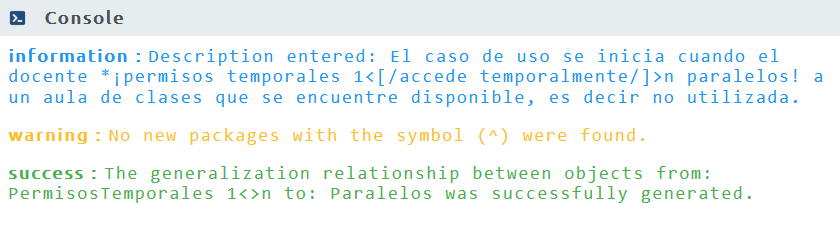
\includegraphics[width=14cm]{img/not-eva-008.png}
	\label{fig:not_eva_008}
	\textbf{\\ ELABORADO: DÚVAL CARVAJAL SUÁREZ}
\end{figure}

\begin{figure}[H]
	\caption{Diagrama de clases generado para la descripción 8.}
	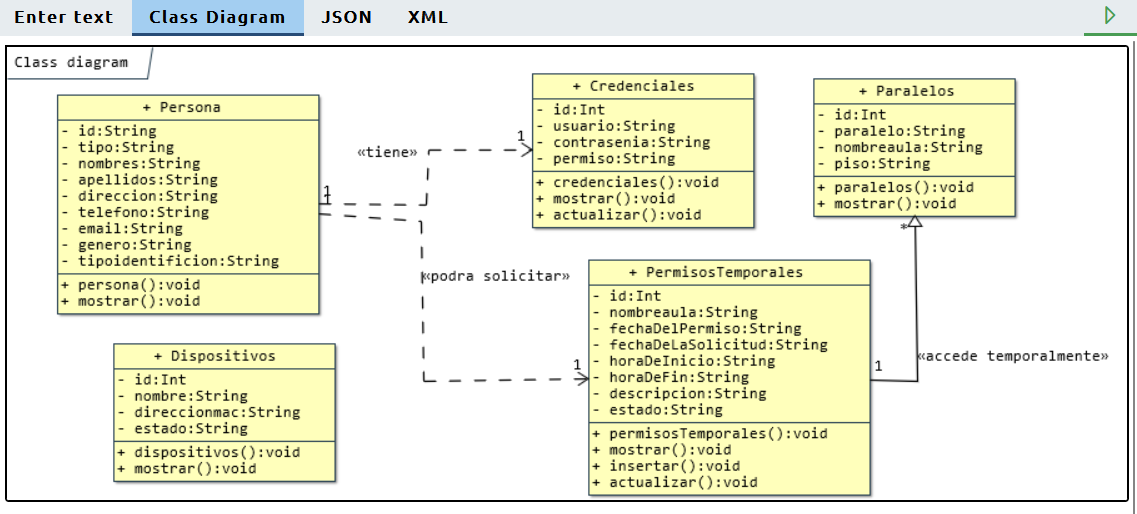
\includegraphics[width=15cm]{img/dc-eva-008.png}
	\label{fig:dc_eva_008}
	\textbf{\\ ELABORADO: DÚVAL CARVAJAL SUÁREZ}
\end{figure}

\begin{lstlisting}
	 9. El docente acepta la vinculación, accede al curso y  *¡paralelos 1<[/tiene control de los/]<n dispositivos! eléctricos y electrónicos ETH. Quedando concluido el caso de uso.
\end{lstlisting}

     \begin{figure}[h!]
	\caption{Mensajes de consola notificando si existe algún error en la escritura de la descripción 9.}
	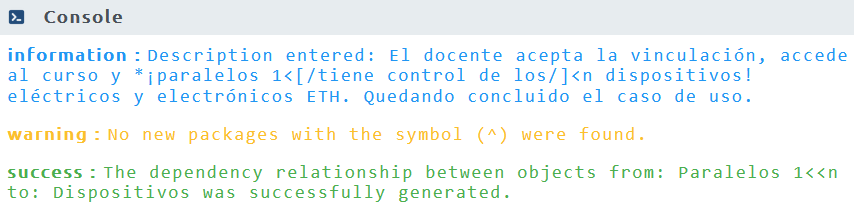
\includegraphics[width=14cm]{img/not-eva-009.png}
	\label{fig:not_eva_009}
	\textbf{\\ ELABORADO: DÚVAL CARVAJAL SUÁREZ}
\end{figure}

\begin{figure}[H]
	\caption{Diagrama de clases generado para la descripción 9.}
	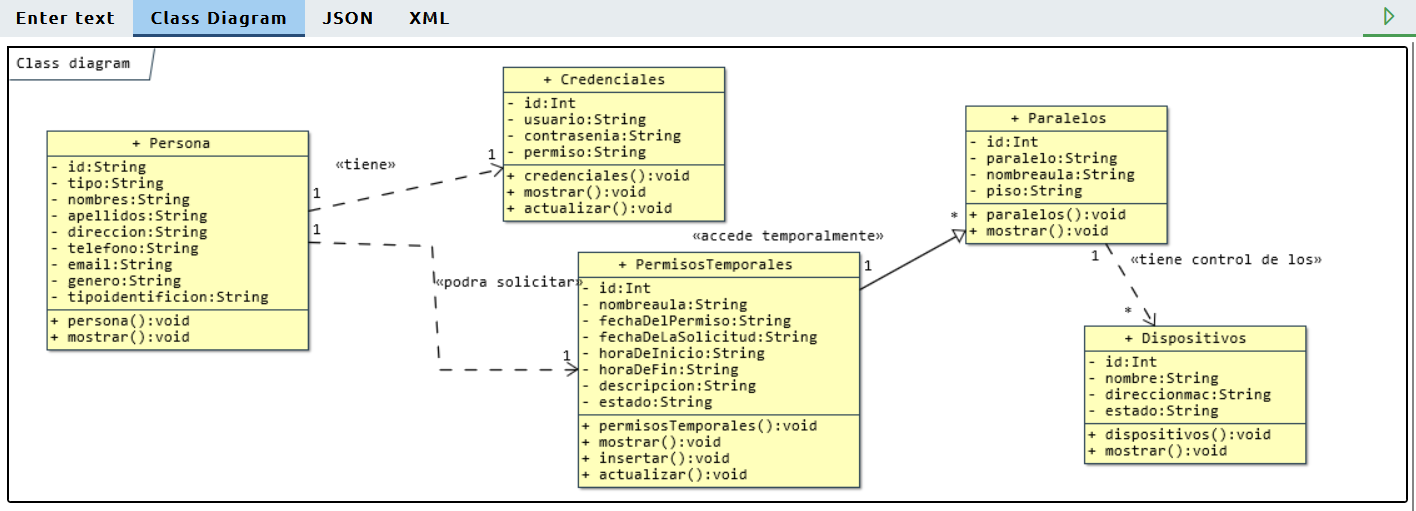
\includegraphics[width=15cm]{img/dc-eva-009.png}
	\label{fig:dc_eva_009}
	\textbf{\\ ELABORADO: DÚVAL CARVAJAL SUÁREZ}
\end{figure}

\begin{lstlisting}
	10. Posterior a la autenticación facial del docente, los estudiantes ingresarán al curso colocando su credencial *(biometrías &-id=int &-serietarjeta=string &-huelladigital=string [+biometrias=empty] [+mostrar=empty]) especial por el Lector RFID, luego el docente ingresará a la aplicación, validará el registro temporal de asistencias y enviará estas asistencias a almacenarse en la base de datos. *¡persona 1<[tiene]<n biometrías!
\end{lstlisting}

     \begin{figure}[h!]
	\caption{Mensajes de consola notificando si existe algún error en la escritura de la descripción 10.}
	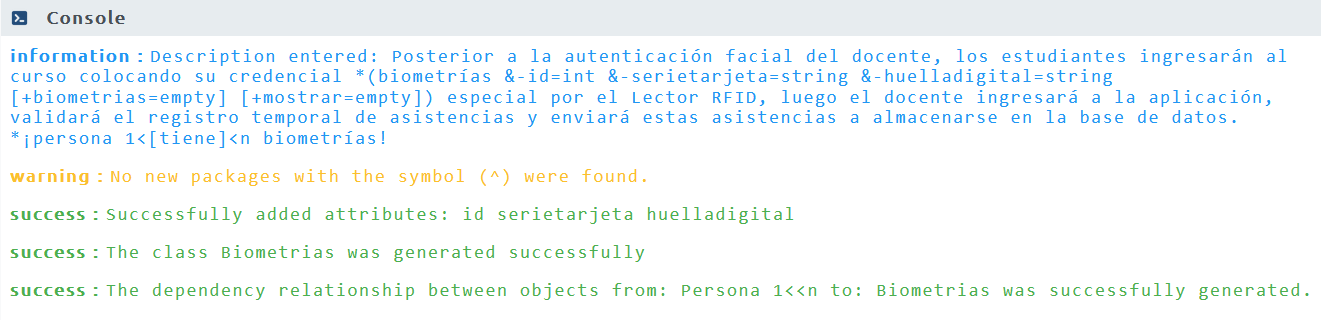
\includegraphics[width=14cm]{img/not-eva-010.png}
	\label{fig:not_eva_010}
	\textbf{\\ ELABORADO: DÚVAL CARVAJAL SUÁREZ}
\end{figure}

\begin{figure}[H]
	\caption{Diagrama de clases generado para la descripción 10.}
	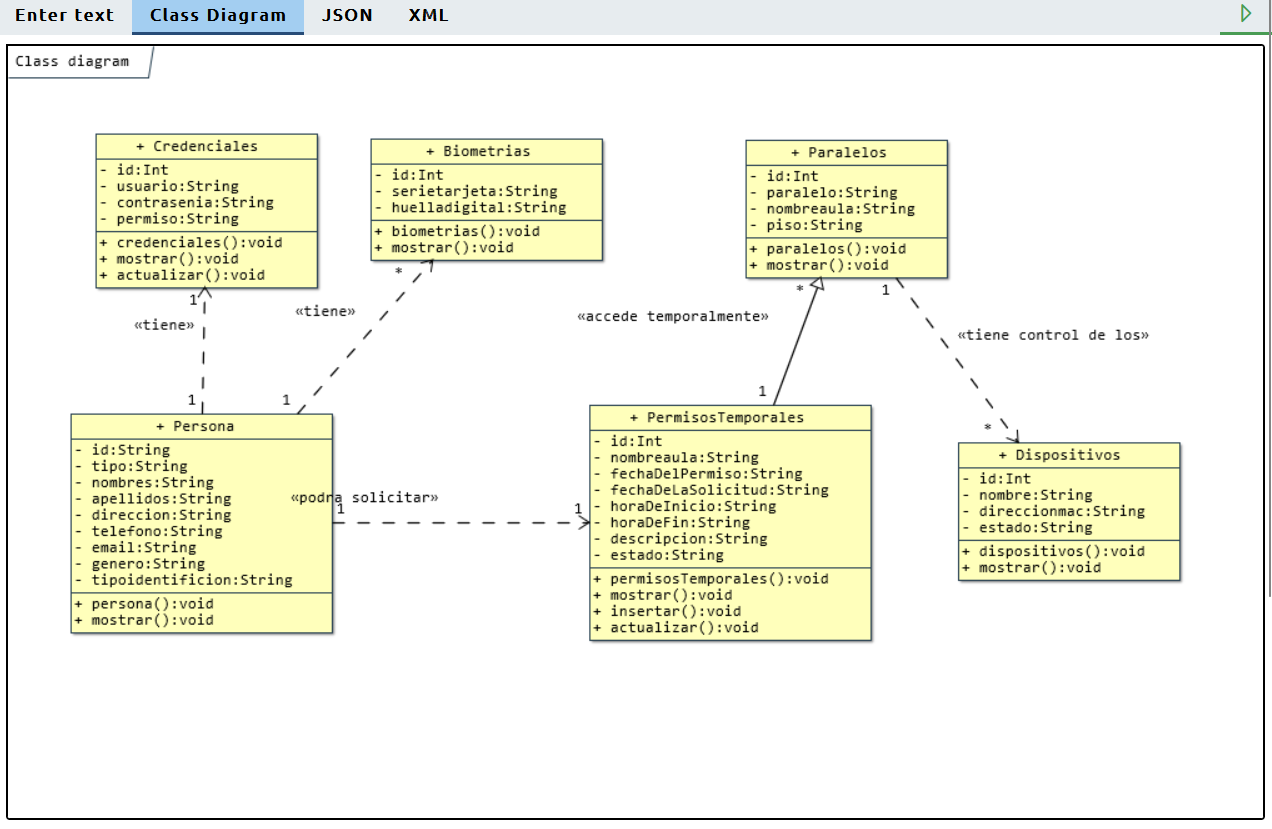
\includegraphics[width=15cm]{img/dc-eva-010.png}
	\label{fig:dc_eva_010}
	\textbf{\\ ELABORADO: DÚVAL CARVAJAL SUÁREZ}
\end{figure}

\begin{lstlisting}
	11. El caso de uso se inicia cuando el docente va a impartir su cátedra en el curso asignado, para ello posterior a su autenticación facial *(fotografías &-id=int &-direccion=string &-nombrefoto=string [+fotografias=empty] [+mostrar=empty] [+insertar=empty]), ingresará a curso acompañado de los estudiantes asignados *¡persona 1<[tiene]>n fotografías! a dicha materia.
\end{lstlisting}

     \begin{figure}[h!]
	\caption{Mensajes de consola notificando si existe algún error en la escritura de la descripción 11.}
	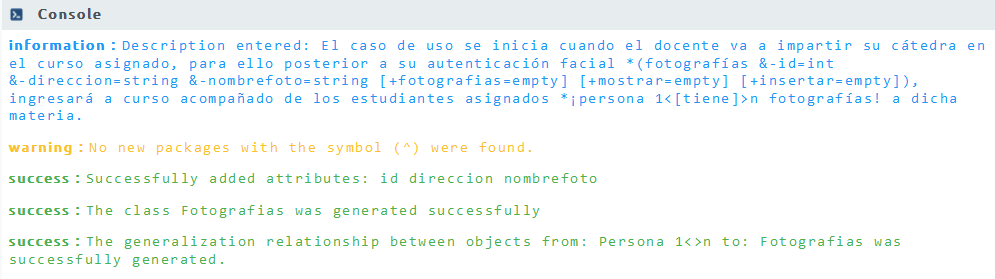
\includegraphics[width=14cm]{img/not-eva-011.png}
	\label{fig:not_eva_011}
	\textbf{\\ ELABORADO: DÚVAL CARVAJAL SUÁREZ}
\end{figure}

\begin{figure}[H]
	\caption{Diagrama de clases generado para la descripción 10.}
	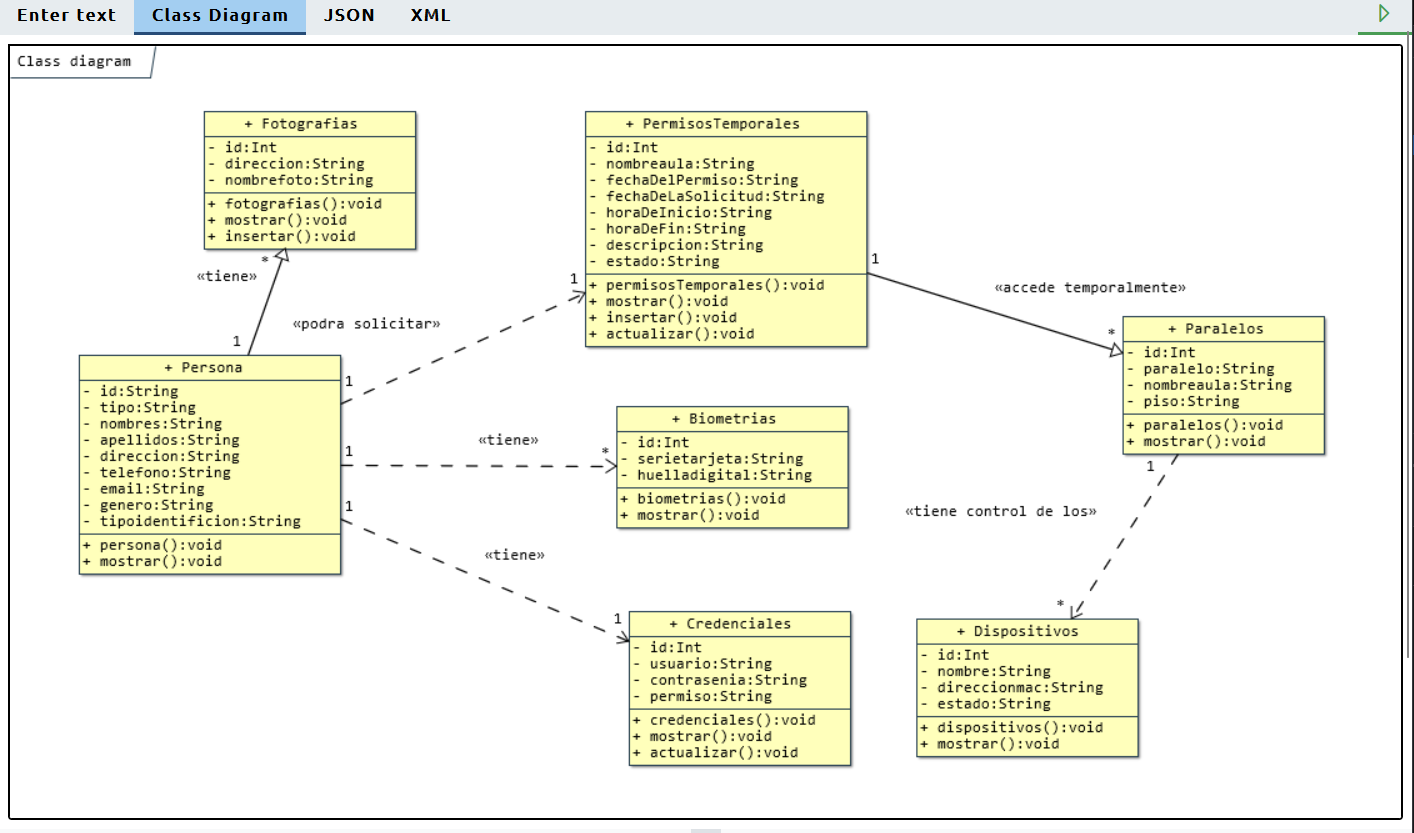
\includegraphics[width=15cm]{img/dc-eva-011.png}
	\label{fig:dc_eva_011}
	\textbf{\\ ELABORADO: DÚVAL CARVAJAL SUÁREZ}
\end{figure}

El diagrama de clases que se observa el figura \ref{fig:dc_eva_011} es el diagrama final que se obtiene luego de ingresar todas las descripciones de los casos de uso. Si se compara con el original se han generado varias clases iguales a las del diagrama de clases original. También se observan los mensajes de retroalimentación que sucede al momento de interpretar cada una de las descripciones.

\begin{table}[h!]
	\caption{Descripción del caso de uso para ingresar al sistema.}
	\label{tab:is_ai}
	\begin{tabular}{| p{3cm} | p{11cm} |}
		\hline
		\textbf{Caso de uso:} & Ingresar al sistema \\ \hline
		\textbf{Actores:} & Docente, Administrador \\ \hline
		\textbf{Propósito:} & Acceder a la aplicación móvil para obtener las diversas opciones que permite el control del curso. \\ \hline
		\textbf{Resumen:} & El actor docente o administrador ingresará las credenciales proporcionadas por la institución, estas se validarán y posterior otorgará el acceso a las opciones.  \\ \hline
		\textbf{Tipo:} & Primario \\ \hline
		\multicolumn{2}{ |c| }{\textbf{Flujo normal}} \\ \hline
	\end{tabular}
	\begin{tabular}{| p{7cm} | p{7cm} |}
		\textbf{Acción del actor} & \textbf{Respuesta del sistema} \\ \hline	
		1. El caso de uso se inicia cuando el actor docente o administrador necesita acceder a la aplicación, para ello ingresa a la aplicación móvil en su dispositivo smartphone.  & \\ \hline
		& 2. Muestra el formulario correspondiente. \\ \hline
		3. El actor docente o administrador ingresa el usuario y contraseña asignados por la institución; y da clic en el botón Ingresar. & \\ \hline
		&4. Válida que los datos sean correctos y muestra el formulario de la ventana principal, dando por concluido el caso de uso. \\ \hline
		\multicolumn{2}{ |c| }{\textbf{Flujos alternos}} \\ \hline
	\end{tabular}
	\begin{tabular}{| p{7cm} | p{7cm} |}
		\textbf{Acción del actor} & \textbf{Respuesta del sistema} \\ \hline	
		& 4.1 Muestra un mensaje de credenciales incorrectas y retorne a la línea 2.  \\ \hline
	\end{tabular}
	\textbf{ \\ ELABORADO: DÚVAL CARVAJAL SUÁREZ}
\end{table}

\begin{table}[h!]
	\caption{Descripción del caso de uso para ingresar al sistema usando el lenguaje de símbolos.}
	\label{tab:is_is_ls}
	\begin{tabular}{| p{3cm} | p{11cm} |}
		\hline
		\textbf{Caso de uso:} & Ingresar al sistema \\ \hline
		\textbf{Actores:} & Docente, Administrador \\ \hline
		\textbf{Propósito:} & Acceder a la aplicación móvil para obtener las diversas opciones que permite el control del curso. \\ \hline
		\textbf{Resumen:} & El actor docente o administrador *(persona) ingresará las *(credenciales) credenciales proporcionadas por la institución, estas se validarán y posterior otorgará el acceso a las opciones.  \\ \hline
		\textbf{Tipo:} & Primario \\ \hline
		\multicolumn{2}{ |c| }{\textbf{Flujo normal}} \\ \hline
	\end{tabular}
	\begin{tabular}{| p{7cm} | p{7cm} |}
		\textbf{Acción del actor} & \textbf{Respuesta del sistema} \\ \hline	
		1. El caso de uso se inicia cuando el actor docente o administrador *(persona \&-id=string \&-tipo=string \&-nombres=string \&-apellidos=string \&-direccion=string \&-telefono=string \&-email=string \&-genero = string \&-tipoidentificion=string [+persona=empty] [+mostrar=empty]) necesita acceder a la aplicación, para ello ingresa a la aplicación móvil en su dispositivo smartphone.  & \\ \hline
		& 2. Muestra el formulario correspondiente. \\ \hline
		3.El actor docente o administrador ingresa el *(credenciales \&-id=int \&-/usuario/=String /y/ \&-/contraseña/=String \&-permiso=string [+credenciales=empyt] [+mostrar=empty] [+actualizar=empty]) asignados por la institución; y da clic en el botón Ingresar. *¡persona 1<[tiene]<1 credenciales! & \\ \hline
		&4. Válida que los datos sean correctos y muestra el formulario de la ventana principal, dando por concluido el caso de uso. \\ \hline
		\multicolumn{2}{ |c| }{\textbf{Flujos alternos}} \\ \hline
	\end{tabular}
	\begin{tabular}{| p{7cm} | p{7cm} |}
		\textbf{Acción del actor} & \textbf{Respuesta del sistema} \\ \hline	
		& 4.1 Muestra un mensaje de credenciales incorrectas y retorne a la línea 2.  \\ \hline
	\end{tabular}
	\textbf{ \\ ELABORADO: DÚVAL CARVAJAL SUÁREZ}
\end{table}

\begin{table}[h!]
	\caption{Descripción del caso de uso para solicitar accesos físicos temporales.}
	\label{tab:sa_ai}
	\begin{tabular}{| p{3cm} | p{11cm} |}
		\hline
		\textbf{Caso de uso:} & Solicitar accesos físicos temporales \\ \hline
		\textbf{Actores:} & Docente \\ \hline
		\textbf{Propósito:} & Solicitar acceso a un aula de clases en un tiempo determinado, teniendo en cuenta que está no se encuentre ocupada por otro docente. \\ \hline
		\textbf{Resumen:} & El docente dentro de la aplicación móvil, escogerá la opción “Permisos cursos” dentro del menú y llenará la información solicitada.  \\ \hline
		\textbf{Tipo:} & Primario \\ \hline
		\multicolumn{2}{ |c| }{\textbf{Flujo normal}} \\ \hline
	\end{tabular}
	\begin{tabular}{| p{7cm} | p{7cm} |}
		\textbf{Acción del actor} & \textbf{Respuesta del sistema} \\ \hline	
		1. El caso de uso se inicia cuando el docente necesita tener acceso temporalmente a un aula de clases que se encuentre disponible no utilizada.   & \\ \hline
		2. El docente, una vez autenticado en la aplicación móvil, ingresará al menú y escogerá la opción “Permisos cursos”.&\\ \hline
		& 3. Muestra el formulario correspondiente. \\ \hline
		4. El docente llenará la información solicitada por la interfaz, que consiste en el curso a solicitar, la fecha del permiso que requiere el acceso, hora de inicio y hora de fin del permiso; y, una descripción donde detallará brevemente la justificación del permiso. Una vez culminado, dará clic en el botón Enviar. &  \\ \hline
		& 5. Mostrará un mensaje de envío correcto de la información, finalizando el caso de uso. \\ \hline
		\multicolumn{2}{ |c| }{\textbf{Flujos alternos}} \\ \hline
	\end{tabular}
	\begin{tabular}{| p{7cm} | p{7cm} |}
		\textbf{Acción del actor} & \textbf{Respuesta del sistema} \\ \hline	
		& 5.1 : Muestra un mensaje de error y retorne a la línea 4.   \\ \hline
	\end{tabular}
	\textbf{ \\ ELABORADO: DÚVAL CARVAJAL SUÁREZ}
\end{table}

\begin{table}[h!]
	\caption{Descripción del caso de uso para solicitar accesos físicos temporales redactado con el lenguaje de símbolos.}
	\label{tab:aft_ai_ls}
	\begin{tabular}{| p{3cm} | p{11cm} |}
		\hline
		\textbf{Caso de uso:} & Solicitar accesos físicos temporales \\ \hline
		\textbf{Actores:} & Docente \\ \hline
		\textbf{Propósito:} & Solicitar acceso a un aula de clases en un tiempo determinado, teniendo en cuenta que está no se encuentre ocupada por otro docente. \\ \hline
		\textbf{Resumen:} & El docente dentro de la aplicación móvil, escogerá la opción “Permisos cursos” dentro del menú y llenará la información solicitada.  \\ \hline
		\textbf{Tipo:} & Primario \\ \hline
		\multicolumn{2}{ |c| }{\textbf{Flujo normal}} \\ \hline
	\end{tabular}
	\begin{tabular}{| p{7cm} | p{7cm} |}
		\textbf{Acción del actor} & \textbf{Respuesta del sistema} \\ \hline	
		1. El caso de uso se inicia cuando el docente necesita tener acceso temporalmente *(permisos temporales [+permisosTemporales=empyt] [+mostrar=empty] [+insertar=empty] [+actualizar=empty]) a un aula de clases que se encuentre disponible no utilizada.   & \\ \hline
		2. El docente, una vez autenticado en la aplicación móvil, ingresará al menú y escogerá la opción “Permisos cursos”.&\\ \hline
		& 3. Muestra el formulario correspondiente. \\ \hline
		4. El docente llenará la información solicitada por la interfaz, que consiste en el curso a solicitar, la *(permisos temporales \&-id=int \&-nombreaula \&-/fecha del permiso/=string /que requiere el acceso,/ \&-fecha de la solicitud=string \&-/hora de inicio/=string /y/ \&-/hora de fin/=string /del permiso; y, una/ \&-/descripción/=string \&-estado=string) donde detallará brevemente la justificación del permiso. Una vez culminado, dará clic en el botón Enviar. *¡persona 1<[podra solicitar]<1 permisos temporales! &  \\ \hline
		& 5. Mostrará un mensaje de envío correcto de la información, finalizando el caso de uso. \\ \hline
		\multicolumn{2}{ |c| }{\textbf{Flujos alternos}} \\ \hline
	\end{tabular}
	\begin{tabular}{| p{7cm} | p{7cm} |}
		\textbf{Acción del actor} & \textbf{Respuesta del sistema} \\ \hline	
		& 5.1 Muestra un mensaje de error y retorne a la línea 4.   \\ \hline
	\end{tabular}
	\textbf{ \\ ELABORADO: DÚVAL CARVAJAL SUÁREZ}
\end{table}

\begin{table}[h!]
	\caption{Descripción del caso de uso para acceder a cursos temporales.}
	\label{tab:ac_ai}
	\begin{tabular}{| p{3cm} | p{11cm} |}
		\hline
		\textbf{Caso de uso:} & Acceder a cursos temporales \\ \hline
		\textbf{Actores:} & Docente \\ \hline
		\textbf{Propósito:} & Ingresar al aula de clases que el docente solicitó un permiso temporal, previo a la autorización del administrador  \\ \hline
		\textbf{Resumen:} & Acceso al curso temporal en la aplicación móvi luego de obtener autorización, donde podrá manipular los dispositivos eléctricos y electrónicos ETH.   \\ \hline
		\textbf{Tipo:} & Secundario \\ \hline
		\multicolumn{2}{ |c| }{\textbf{Flujo normal}} \\ \hline
	\end{tabular}
	\begin{tabular}{| p{7cm} | p{7cm} |}
		\textbf{Acción del actor} & \textbf{Respuesta del sistema} \\ \hline	
		1. El caso de uso se inicia cuando el docente accede temporalmente a un aula de clases que se encuentre disponible, es decir no utilizada.    & \\ \hline
		2. El docente, una vez autenticado en la aplicación móvil, ingresará a la pestaña de “Cursos Temporales”.&\\ \hline
		&  3. Mostrará el listado de los cursos temporales autorizados.\\ \hline
		4. Escoge un determinado curso dentro de la aplicación &  \\ \hline
		& 5. Verifica que tenga acceso al curso validando si encuentra dentro del rango de horas solicitadas. \\ \hline
		& Vincula el celular a través de bluetooth con el Sistema Arduino. \\ \hline
		7. El docente acepta la vinculación, accede al curso y tiene control de los eléctricos y electrónicos ETH. Quedando concluido el caso de uso. & \\ \hline
		\multicolumn{2}{ |c| }{\textbf{Flujos alternos}} \\ \hline
	\end{tabular}
	\begin{tabular}{| p{7cm} | p{7cm} |}
		\textbf{Acción del actor} & \textbf{Respuesta del sistema} \\ \hline	
		& 5.1 Muestra un mensaje de error y retorne a la línea 3.    \\ \hline
	\end{tabular}
	\textbf{ \\ ELABORADO: DÚVAL CARVAJAL SUÁREZ}
\end{table}

\begin{table}[h!]
	\caption{Descripción del caso de uso para Acceder a cursos temporales.}
	\label{tab:ac_ai_ls}
	\begin{tabular}{| p{3cm} | p{11cm} |}
		\hline
		\textbf{Caso de uso:} & Acceder a cursos temporales \\ \hline
		\textbf{Actores:} & Docente \\ \hline
		\textbf{Propósito:} & Ingresar al aula de clases *(paralelos \&-id=int \&-paralelo=string \&-nombreaula=string \&-piso=string [+paralelos=empty] [+mostrar=empty]) que el docente solicitó un permiso temporal, previo a la autorización del administrador  \\ \hline
		\textbf{Resumen:} & Acceso al curso temporal en la aplicación móvi  luego de obtener autorización, donde podrá manipular los dispositivos *(dispositivos \&-id=int \&-nombre=string \&-direccionmac \&-estado=string [+dispositivos=empty] [+mostrar=empty]) eléctricos y electrónicos ETH.   \\ \hline
		\textbf{Tipo:} & Secundario \\ \hline
		\multicolumn{2}{ |c| }{\textbf{Flujo normal}} \\ \hline
	\end{tabular}
	\begin{tabular}{| p{7cm} | p{7cm} |}
		\textbf{Acción del actor} & \textbf{Respuesta del sistema} \\ \hline	
		1. El caso de uso se inicia cuando el docente *¡permisos temporales 1<[/accede temporalmente/]>n paralelos! a un aula de clases que se encuentre disponible, es decir no utilizada.    & \\ \hline
		2. El docente, una vez autenticado en la aplicación móvil, ingresará a la pestaña de “Cursos Temporales”.&\\ \hline
		&  3. Mostrará el listado de los cursos temporales autorizados.\\ \hline
		4. Escoge un determinado curso dentro de la aplicación &  \\ \hline
		& 5. Verifica que tenga acceso al curso validando si encuentra dentro del rango de horas solicitadas. \\ \hline
		& Vincula el celular a través de bluetooth con el Sistema Arduino. \\ \hline
		7. El docente acepta la vinculación, accede al curso y  *¡paralelos 1<[/tiene control de los/]<n dispositivos! eléctricos y electrónicos ETH. Quedando concluido el caso de uso. & \\ \hline
		\multicolumn{2}{ |c| }{\textbf{Flujos alternos}} \\ \hline
	\end{tabular}
	\begin{tabular}{| p{7cm} | p{7cm} |}
		\textbf{Acción del actor} & \textbf{Respuesta del sistema} \\ \hline	
		& 5.1 Muestra un mensaje de error y retorne a la línea 3.    \\ \hline
	\end{tabular}
	\textbf{ \\ ELABORADO: DÚVAL CARVAJAL SUÁREZ}
\end{table}

\begin{table}[h!]
	\caption{Descripción del caso de uso para registrar asistencia de estudiantes.}
	\label{tab:rae_ai}
	\begin{tabular}{| p{3cm} | p{11cm} |}
		\hline
		\textbf{Caso de uso:} & Registrar asistencia de estudiantes \\ \hline
		\textbf{Actores:} & Docente, Estudiante. \\ \hline
		\textbf{Propósito:} & Registrar la asistencia de los estudiantes que ingresarán al aula de clases, previo a mantener cátedra con el docente asignado.  \\ \hline
		\textbf{Resumen:} & Posterior a la autenticación facial del docente, los estudiantes ingresarán al curso colocando su credencial especial por el Lector RFID, luego el docente ingresará a la aplicación, validará el registro temporal de asistencias y enviará estas asistencias a almacenarse en la base de datos.    \\ \hline
		\textbf{Tipo:} & Secundario \\ \hline
		\multicolumn{2}{ |c| }{\textbf{Flujo normal}} \\ \hline
	\end{tabular}
	\begin{tabular}{| p{7cm} | p{7cm} |}
		\textbf{Acción del actor} & \textbf{Respuesta del sistema} \\ \hline	
		1. El caso de uso se inicia cuando el docente va a impartir su cátedra en el curso asignado, para ello posterior a su autenticación facial , ingresará a curso acompañado de los estudiantes asignados a dicha materia.     & \\ \hline
		2. Los estudiantes ingresarán al curso, ordenados e independientes; y, colocarán su credencial especial en el Lector RFID. &\\ \hline
		&  3. Obtiene el código de la tarjeta, válida los datos del estudiante y registra su asistencia temporal.\\ \hline
		& 4. Mostrará en la interface de usuario, la asistencia de ingreso a la materia de todos los estudiantes.  \\ \hline
		5. El docente deberá dar clic en el ícono de “Actualizar Asistencias”, para obtener las asistencias e inasistencias temporales de cada alumno. & \\ \hline
		& 6. En la interfaz de usuario, se actualizará las asistencias de los estudiantes que han utilizado la credencial especial. \\ \hline
		7. El docente verificará que las asistencias se encuentren correctas, y dará clic en el ícono de “Guardar Asistencias” para almacenar definitivamente las asistencias en la base de datos. & \\ \hline
	\end{tabular}
\end{table}

\begin{table}[h!]
	\begin{tabular}{| p{7cm} | p{7cm} |}
		\hline
		&  8. Mostrará un mensaje de confirmación, para registrar la información. \\ \hline
		9. El docente confirmará a través del respectivo botón de la aplicación móvil, subir la asistencia a la base de datos. & \\ \hline
		& 10. Mostrará mensaje de éxito, actualiza la lista de estudiantes con la respectiva asistencia, y bloquea el botón “Registrar Asistencia”. Con esto finaliza el caso de uso. \\ \hline
		\multicolumn{2}{ |c| }{\textbf{Flujos alternos}} \\ \hline
	\end{tabular}
	\begin{tabular}{| p{7cm} | p{7cm} |}
		\textbf{Acción del actor} & \textbf{Respuesta del sistema} \\ \hline	
		& 5.1 Muestra un mensaje de error y retorne a la línea 3.    \\ \hline
	\end{tabular}
	\textbf{ \\ ELABORADO: DÚVAL CARVAJAL SUÁREZ}
\end{table}

\begin{table}[h!]
	\caption{Descripción del caso de uso para Registrar asistencia de estudiantes redactado con el lenguaje de símbolos.}
	\label{tab:rae_ai_ls}
	\begin{tabular}{| p{3cm} | p{11cm} |}
		\hline
		\textbf{Caso de uso:} & Acceder a cursos temporales \\ \hline
		\textbf{Actores:} & Docente, Estudiante. \\ \hline
		\textbf{Propósito:} & Registrar la asistencia de los estudiantes que ingresarán al aula de clases, previo a mantener cátedra con el docente asignado.  \\ \hline
		\textbf{Resumen:} & Posterior a la autenticación facial del docente, los estudiantes ingresarán al curso colocando su credencial *(biometrías \&-id=int \&-serietarjeta=string \&-huelladigital=string [+biometrias=empty] [+mostrar=empty]) especial por el Lector RFID, luego el docente ingresará a la aplicación, validará el registro temporal de asistencias y enviará estas asistencias a almacenarse en la base de datos. *¡persona 1<[tiene]<n biometrías!    \\ \hline
		\textbf{Tipo:} & Secundario \\ \hline
		\multicolumn{2}{ |c| }{\textbf{Flujo normal}} \\ \hline
	\end{tabular}
	\begin{tabular}{| p{7cm} | p{7cm} |}
		\textbf{Acción del actor} & \textbf{Respuesta del sistema} \\ \hline	
		1. El caso de uso se inicia cuando el docente va a impartir su cátedra en el curso asignado, para ello posterior a su autenticación facial *(fotografías \&-id=int \&-direccion=string \&-nombrefoto=string [+fotografias=empty] [+mostrar=empty] [+insertar=empty]), ingresará a curso acompañado de los estudiantes asignados *¡persona 1<[tiene]>n fotografías! a dicha materia.     & \\ \hline
		2. Los estudiantes ingresarán al curso, ordenados e independientes; y, colocarán su credencial especial en el Lector RFID. &\\ \hline
	\end{tabular}
\end{table}

\begin{table}[h!]
	\begin{tabular}{| p{7cm} | p{7cm} |}
		\hline
		&  3. Obtiene el código de la tarjeta, válida los datos del estudiante y registra su asistencia temporal.\\ \hline
		& 4. Mostrará en la interface de usuario, la asistencia de ingreso a la materia de todos los estudiantes.  \\ \hline
		5. El docente deberá dar clic en el ícono de “Actualizar Asistencias”, para obtener las asistencias e inasistencias temporales de cada alumno. & \\ \hline
		& 6. En la interfaz de usuario, se actualizará las asistencias de los estudiantes que han utilizado la credencial especial. \\ \hline
		7. El docente verificará que las asistencias se encuentren correctas, y dará clic en el ícono de “Guardar Asistencias” para almacenar definitivamente las asistencias en la base de datos. & \\ \hline
		&  8. Mostrará un mensaje de confirmación, para registrar la información. \\ \hline
		9. El docente confirmará a través del respectivo botón de la aplicación móvil, subir la asistencia a la base de datos. & \\ \hline
		& 10. Mostrará mensaje de éxito, actualiza la lista de estudiantes con la respectiva asistencia, y bloquea el botón “Registrar Asistencia”. Con esto finaliza el caso de uso. \\ \hline
		\multicolumn{2}{ |c| }{\textbf{Flujos alternos}} \\ \hline
	\end{tabular}
	\begin{tabular}{| p{7cm} | p{7cm} |}
		\textbf{Acción del actor} & \textbf{Respuesta del sistema} \\ \hline	
		& 5.1 Muestra un mensaje de error y retorne a la línea 3.    \\ \hline
	\end{tabular}
	\textbf{ \\ ELABORADO: DÚVAL CARVAJAL SUÁREZ}
\end{table}


	\setcounter{chapter}{5}
\setcounter{section}{0}
\part{CONCLUSIONES Y RECOMENDACIONES}

\section{Conclusiones}

\begin{itemize}
	\item Con la utilización de un lenguaje de símbolos que permita estar combinado con las descripciones de los casos de uso escritos en texto natural, además que permita detallar datos técnicos que intervendrán en la generación del sistema informático, logra disminuir un poco el tiempo en la creación de este diagrama de clases. Previamente el desarrollador podrá utilizar la librería en su propio proyecto o utilizar la aplicación web de demostración.
	\item Para los usuarios que utilizan la herramienta TDDT4IoTS al momento de interpretar las descripciones de los casos de uso con la librería desarrollada, les permite identificar de forma más rápida donde están cometiendo errores al momento de utilizar los símbolos respectivos.
	\item La aplicación de demostración sobre cómo funciona la librería servirá para los desarrolladores que necesiten generar un diagrama de clases de una forma rápida dependiendo del sistema informático al que se estén enfrentando. La librería puede ser descargada para que cada desarrollador personalice la forma en cómo y con que genere el diagrama de clases, obteniendo una aplicativo que funcione con todos los proyectos que desarrolle a futuro.   
	\item Se logro obtener un solo archivo de tipo .js que puede ser exportado a cualquier tipo de proyecto web. Esto beneficia a muchas aplicaciones que necesiten de la interpretación de los casos de uso que usen los símbolos de una forma rápida y sin tener que instalar programas externos para su correcto funcionamiento.
\end{itemize}

\newpage
\section{Recomendaciones}
	
\begin{itemize}
	\item La librería desarrollada en el lenguaje javascript puede ser fácilmente escalable. Se puede desarrollar un proyecto npm y subirlo al repositorio oficial para que pueda ser utilizado mediante proyectos que utilicen como servidor de aplicaciones Node.js. 
	\item Durante la elaboración de la retroalimentación sobre cómo utilizar los símbolos para escribir las descripciones de los casos de uso, se pueden realizar trabajos posteriores sobre como identificar la posición exacta del error que se está cometiendo. Se pueden utilizar una serie de colores que permita identificar los caracteres donde se encuentren las anomalías.
	\item Para lograr que la librería pueda ser mejorada, se puede pensar en publicar el código fuente en una plataforma web como lo es GitHub y permitir que otros desarrolladores  mejoren la librería para llegar a un mayor alcance en la comunidad de programadores a nivel mundial.
	\item Para lograr un mayor alance sobre las tecnologías de desarrollo que existen actualmente, y con las que en un futuro serán desarrolladas. Se podrá crear un proyecto que este desplegado en un servidor que este en la nube para crear un servicio web que realice el mismo proceso de la librería, con la ventaja que podrá ser utilizado en casi todos los tipos de proyectos que existen. Se podrá obtener los resultados del proyecto de forma clara y remota.  
\end{itemize}	
	\part{BIBLIOGRAFÍA}
	
\def\thispagestyle#1{}
\printbibliography[title={Referencias}]                                                                         
	\setcounter{chapter}{6}
\setcounter{section}{0}
\part{ANEXOS}

\section{Interfaz principal de aplicación demostrativa de la librería}
\begin{figure}[H]
	\centering
	%\caption{Interfaz principal de aplicación demostrativa de la librería.}
	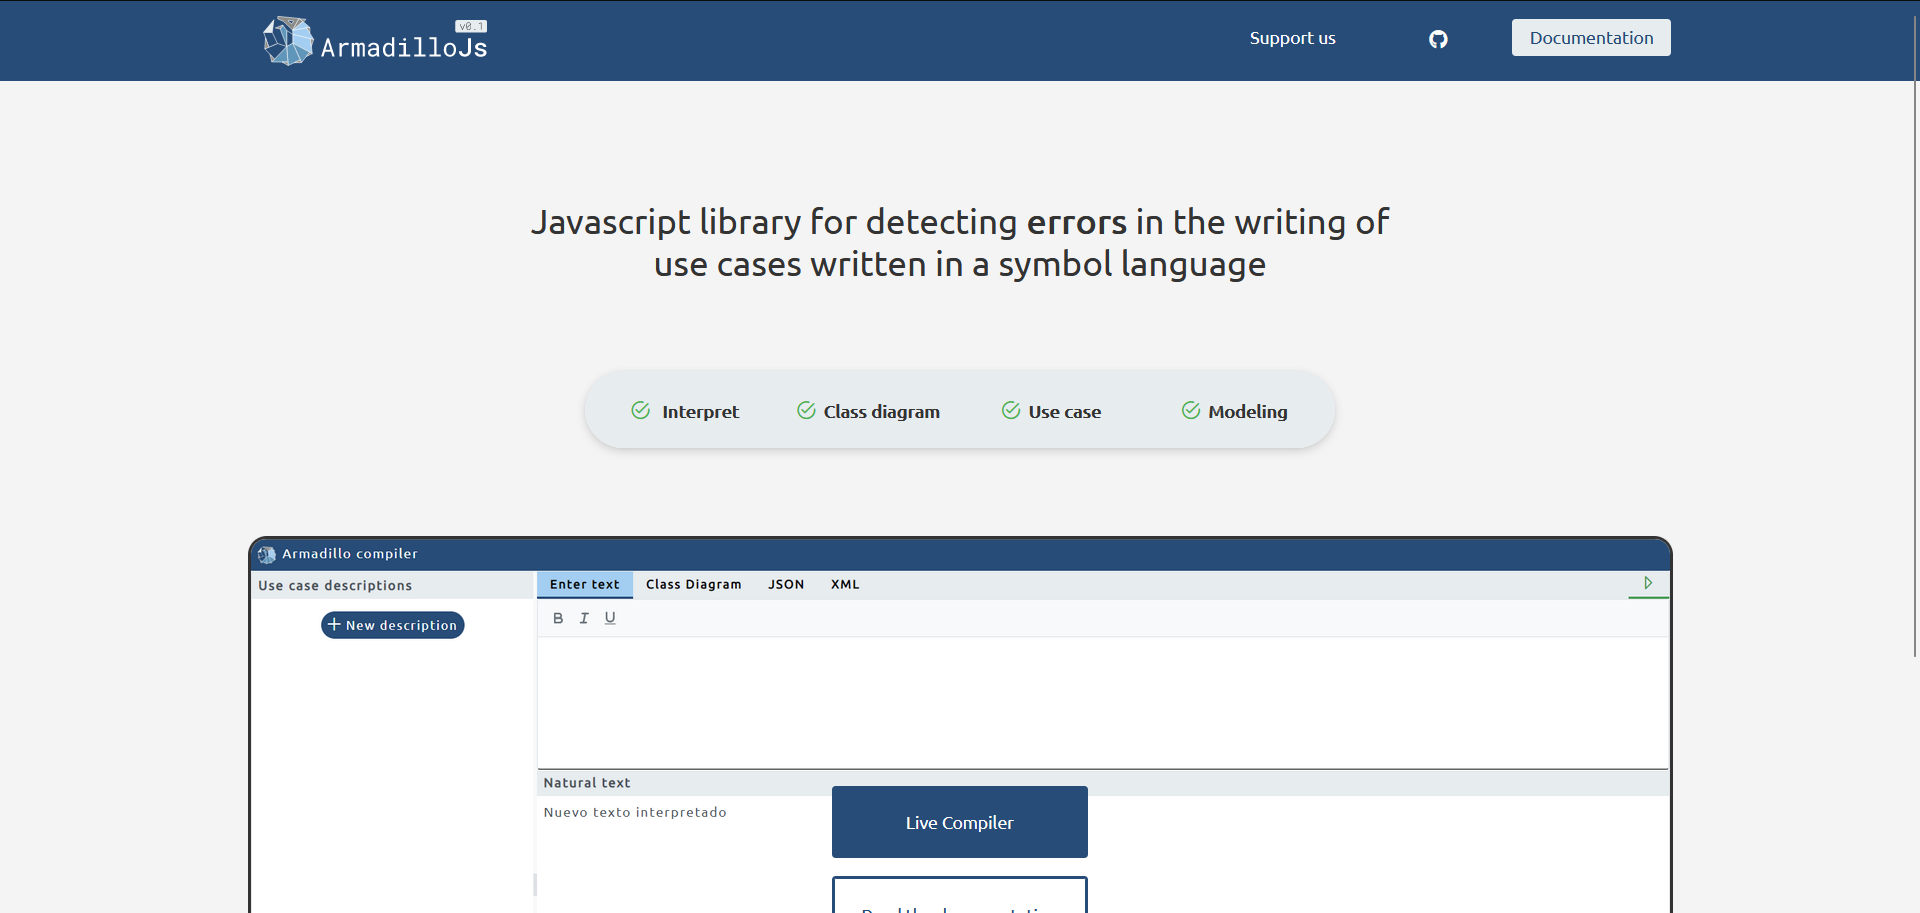
\includegraphics[width=15cm]{img/anexo1.png}
	\label{fig:anexo1}
	%\textbf{\\ FUENTE: PROPIA \\ ELABORADO: DÚVAL CARVAJAL SUÁREZ}
\end{figure} 

\section{Interfaz donde se ingresarán las descripciones de los casos de uso a interpretar}
\begin{figure}[H]
	\centering
	%\caption{Interfaz donde se ingresarán las descripciones de los casos de uso a interpretar.}
	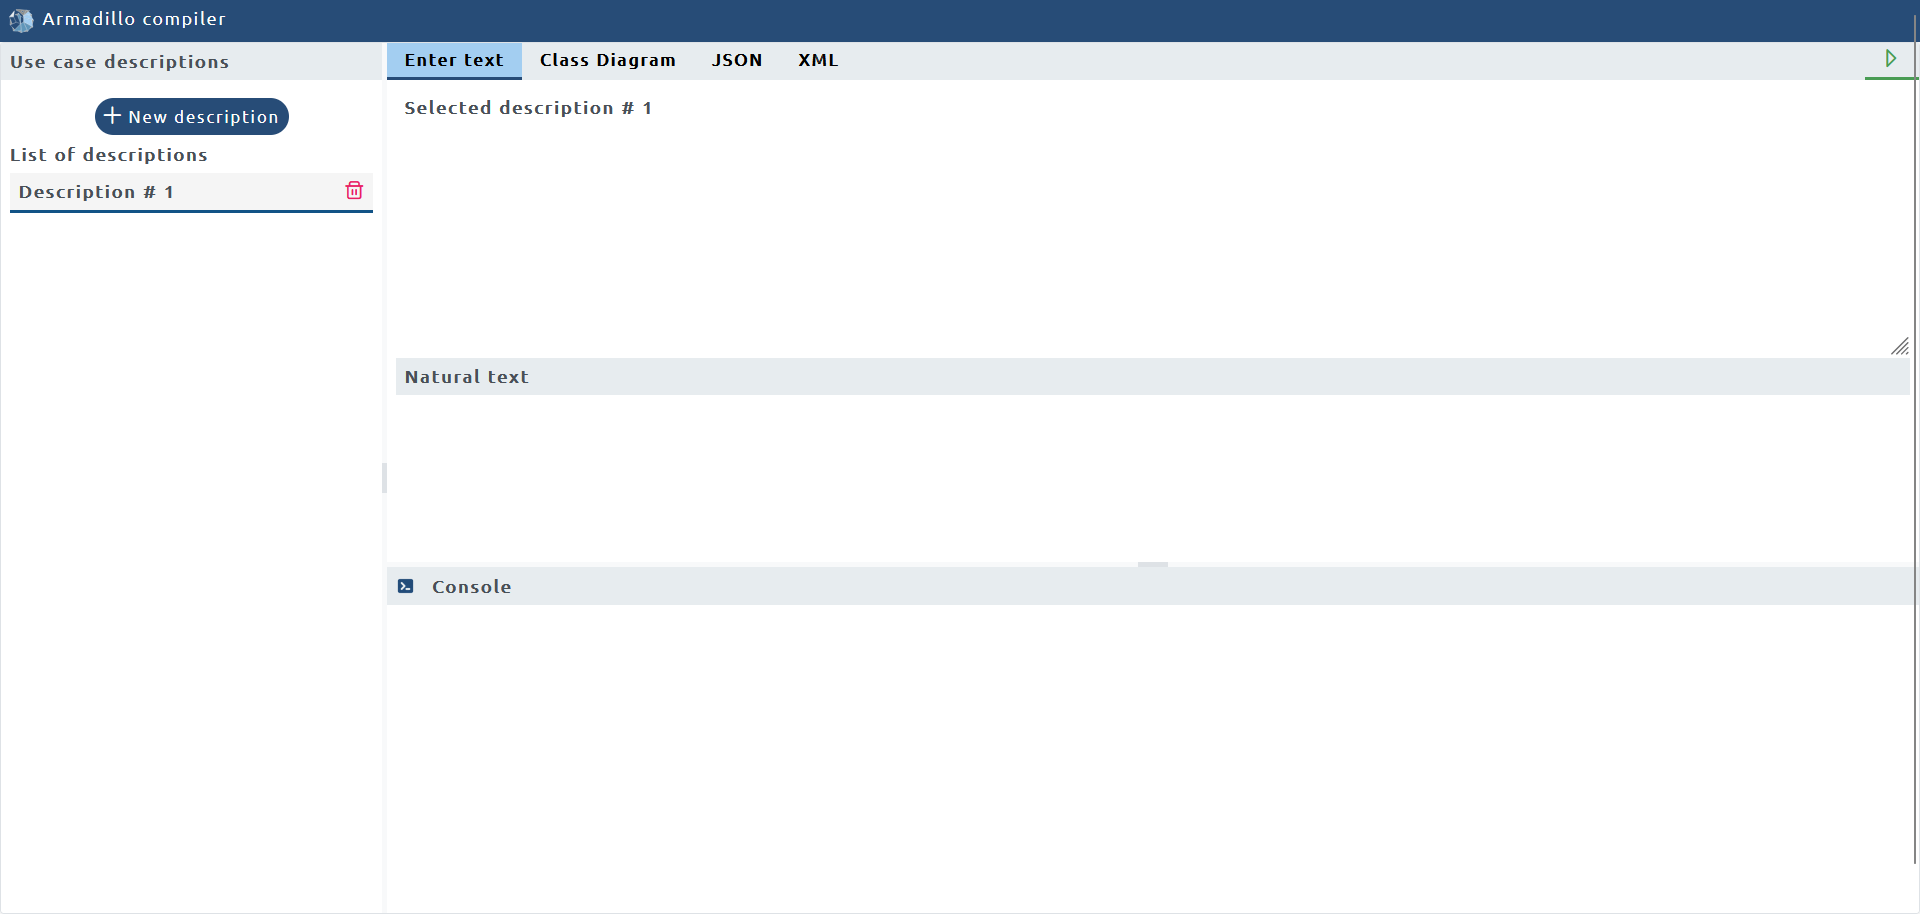
\includegraphics[width=15cm]{img/anexo2.png}
	\label{fig:anexo2}
%	\textbf{\\ FUENTE: PROPIA \\ ELABORADO: DÚVAL CARVAJAL SUÁREZ}
\end{figure} 

\section{Descripción del caso de uso interpretada con su respectiva retroalimentación}
\begin{figure}[H]
	\centering
	%\caption{Descripción del caso de uso interpretada con su respectiva retroalimentación.}
	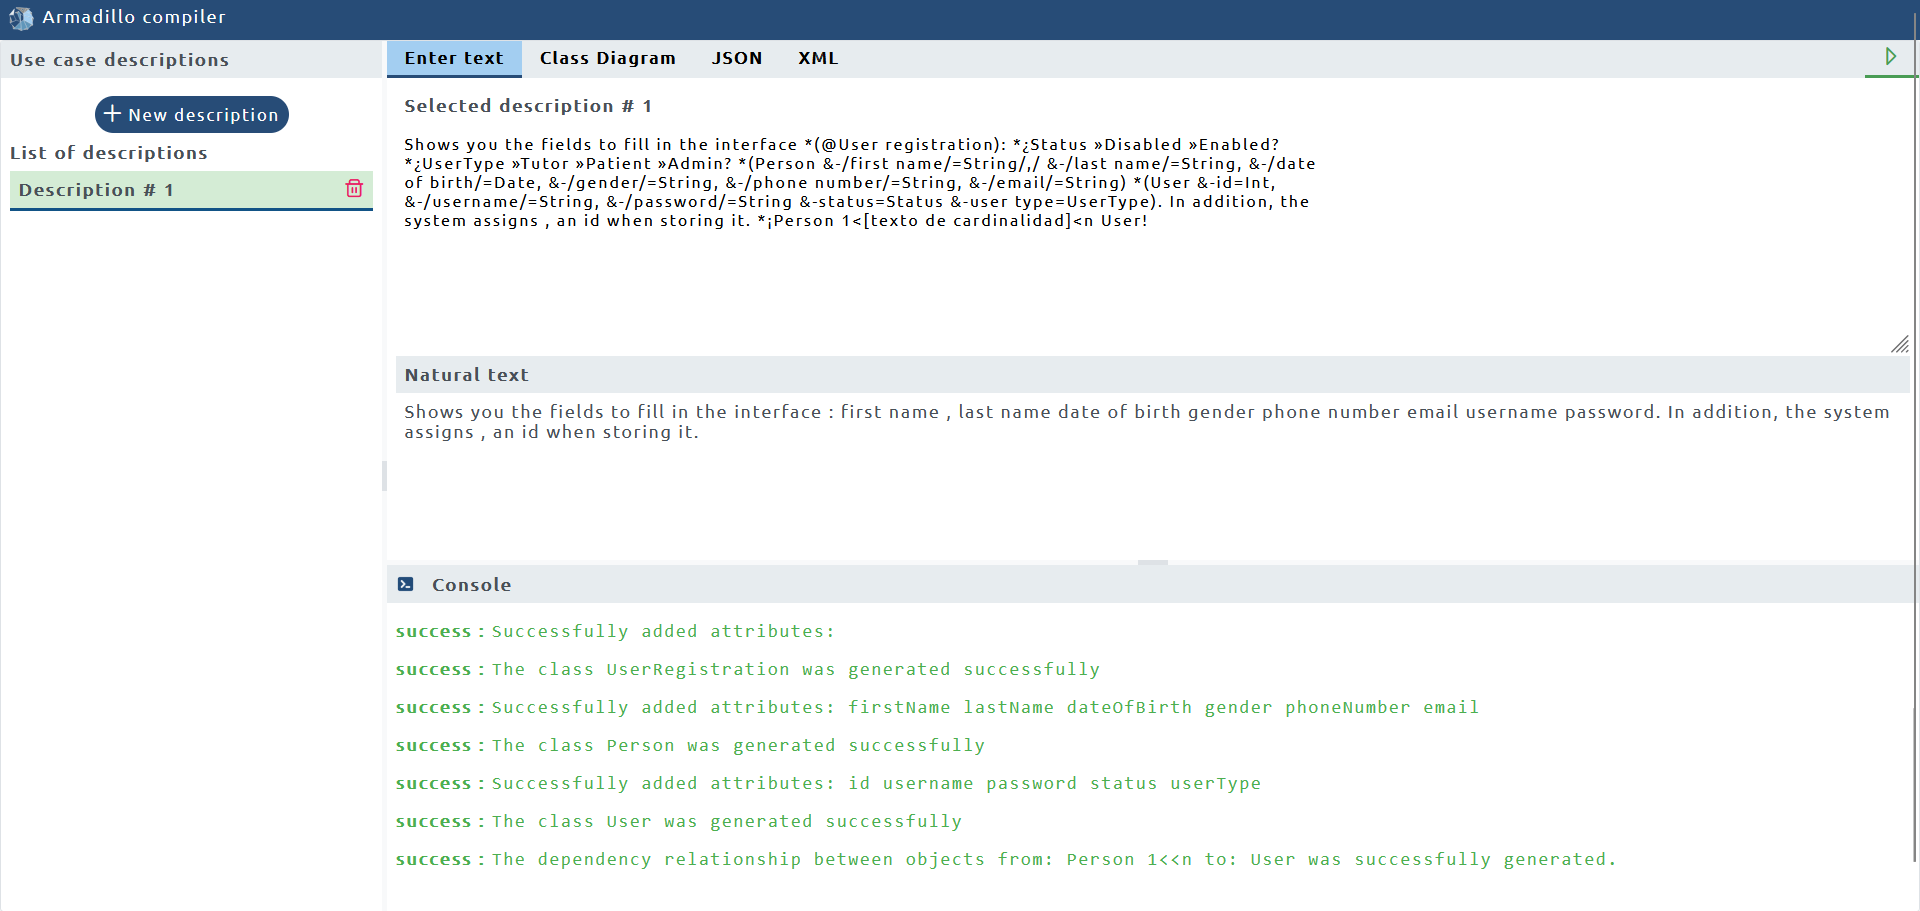
\includegraphics[width=15cm]{img/anexo3.png}
	\label{fig:anexo3}
	%\textbf{\\ FUENTE: PROPIA \\ ELABORADO: DÚVAL CARVAJAL SUÁREZ}
\end{figure} 

\section{Diagrama de clases generado por la librería usando una librería externa denominada jsUML2}
\begin{figure}[H]
	\centering
	%\caption{Diagrama de clases generado por la librería usando una librería externa denominada jsUML2.}
	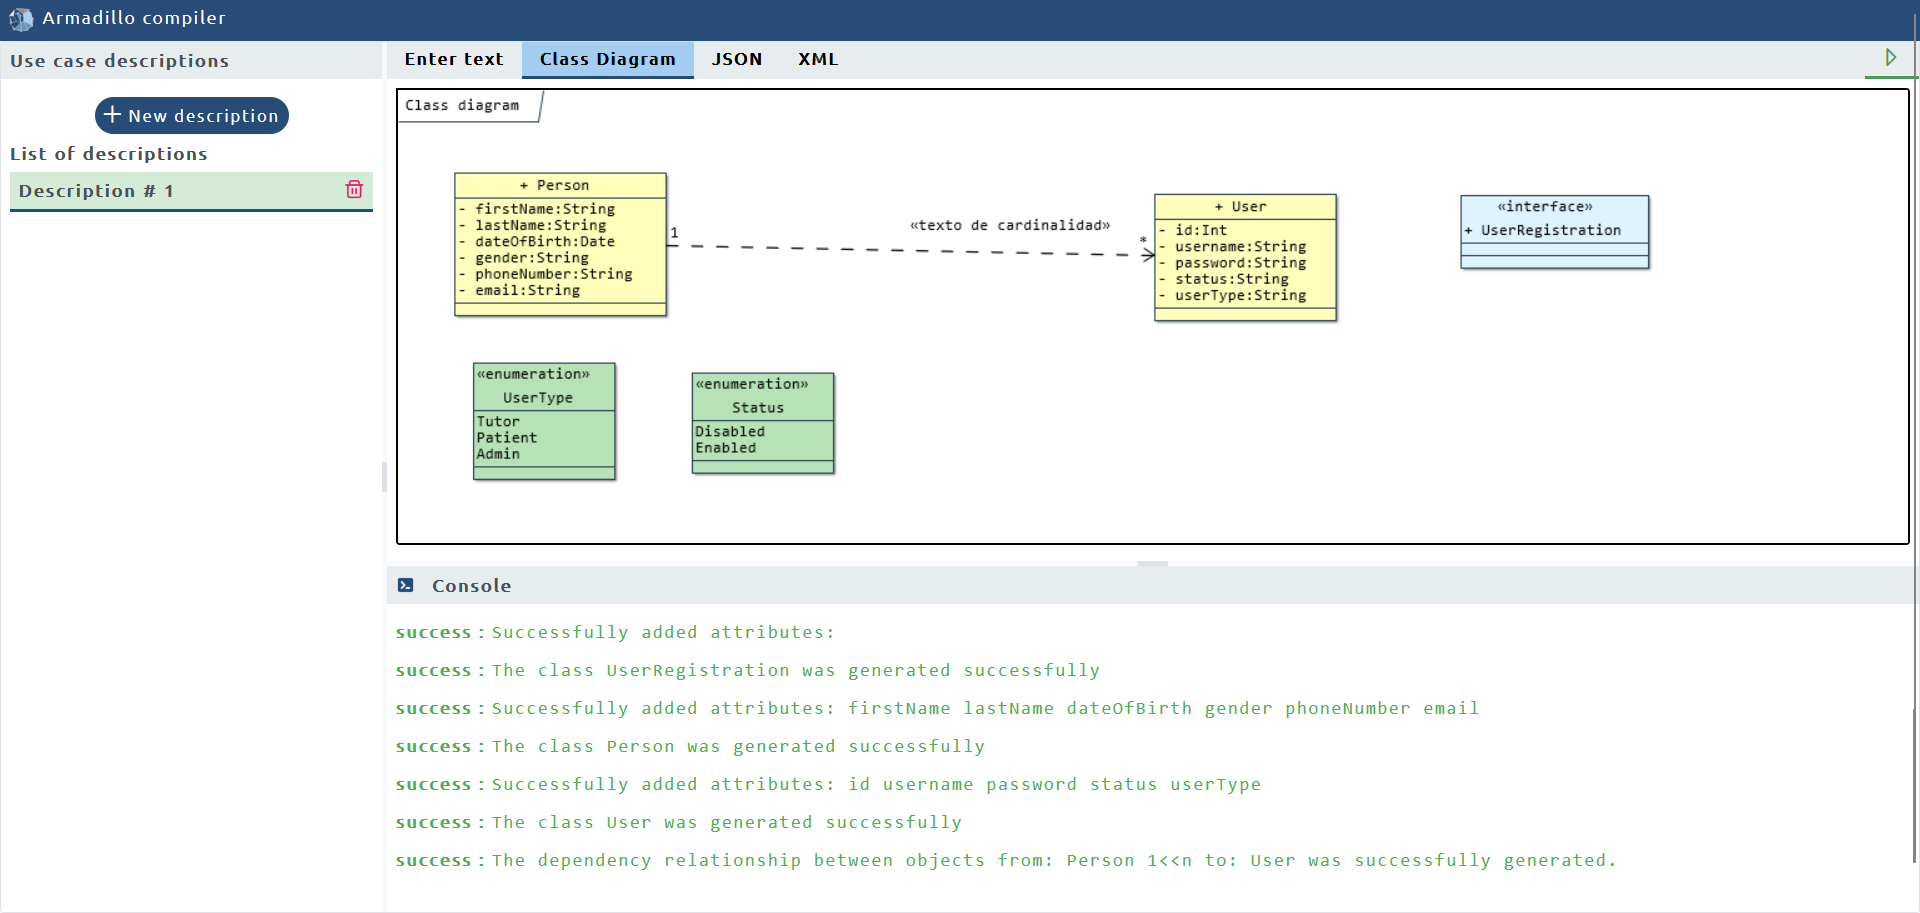
\includegraphics[width=15cm]{img/anexo4.png}
	\label{fig:anexo4}
	%\textbf{\\ FUENTE: PROPIA \\ ELABORADO: DÚVAL CARVAJAL SUÁREZ}
\end{figure} 

\section{Estructura JSON generada por la librería}
\begin{figure}[H]
	\centering
	%\caption{Estructura JSON generada por la librería.}
	\includegraphics[width=15cm]{img/anexo5.png}
	\label{fig:anexo5}
	%\textbf{\\ FUENTE: PROPIA \\ ELABORADO: DÚVAL CARVAJAL SUÁREZ}
\end{figure} 

\section{XML generado por la librería}
\begin{figure}[H]
	\centering
	%\caption{XML generado por la librería.}
	\includegraphics[width=15cm]{img/anexo6.png}
	\label{fig:anexo6}
	%\textbf{\\ FUENTE: PROPIA \\ ELABORADO: DÚVAL CARVAJAL SUÁREZ}
\end{figure} 

\section{Error detectado en la descripción del caso de uso}
\begin{figure}[H]
	%\centering
%	\caption{Error detectado en la descripción del caso de uso}
	\includegraphics[width=15cm]{img/anexo7.png}
	\label{fig:anexo7}
	%\textbf{\\ FUENTE: PROPIA \\ ELABORADO: DÚVAL CARVAJAL SUÁREZ}
\end{figure} 
	
\end{document}